%2multibyte Version: 5.50.0.2960 CodePage: 1252
%\usepackage{mathpazo}


\documentclass[notes=show,smaller,handout]{beamer}
%%%%%%%%%%%%%%%%%%%%%%%%%%%%%%%%%%%%%%%%%%%%%%%%%%%%%%%%%%%%%%%%%%%%%%%%%%%%%%%%%%%%%%%%%%%%%%%%%%%%%%%%%%%%%%%%%%%%%%%%%%%%%%%%%%%%%%%%%%%%%%%%%%%%%%%%%%%%%%%%%%%%%%%%%%%%%%%%%%%%%%%%%%%%%%%%%%%%%%%%%%%%%%%%%%%%%%%%%%%%%%%%%%%%%%%%%%%%%%%%%%%%%%%%%%%%
\usepackage{amssymb}
\usepackage{amsmath}
\usepackage{graphicx}
\usepackage{hyperref}
\usepackage{multimedia}
\usepackage{epstopdf}
\usepackage{color}
\usepackage{tikz}


\setcounter{MaxMatrixCols}{10}
\newtheorem{remark}{Remark}[section]
\newtheorem{proposition}{Proposition}[section]
\newtheorem{interpretation}{Interpretation}[section]
\newtheorem{goal}{Goal}[section]
\newtheorem{statement}{Statement}[section]
\newtheorem{aes}{Aim \& Scope}[section]
\newtheorem{exercise}{Exercise}[section]
\renewcommand{\Pr}{P}

\newcommand{\mbf}[1]{\mathbf{#1}}
\newcommand{\beq}{\begin{equation}}
\newcommand{\eeq}{\end{equation}}
\newcommand{\bea}{\begin{eqnarray}}
\newcommand{\eea}{\end{eqnarray}}
\newcommand{\ba}{\begin{array}}
\newcommand{\ea}{\end{array}}
\newcommand{\bi}{\begin{itemize}}
\newcommand{\ei}{\end{itemize}}
\newcommand{\ben}{\begin{enumerate}}
\newcommand{\een}{\end{enumerate}}
\newcommand{\nn}{\nonumber}
\newcommand{\N}{\mathcal{N}}

\newenvironment{stepenumerate}{\begin{enumerate}[<+->]}{\end{enumerate}}
\newenvironment{stepitemize}{\begin{itemize}[<+->]}{\end{itemize} }
\newenvironment{stepenumeratewithalert}{\begin{enumerate}[<+-| alert@+>]}{\end{enumerate}}
\newenvironment{stepitemizewithalert}{\begin{itemize}[<+-| alert@+>]}{\end{itemize} }
\usetheme{Madrid}


\begin{document}

\title[S110015]{Probability I}
\subtitle{Lecture 5, Lecture 6, Lecture 7}
\author[La Vecchia]{Davide La Vecchia}
\date{Spring Semester 2020}
\maketitle



\begin{frame}%
%EndExpansion

\frametitle{Continuous Distributions}

\begin{example}[Standard \& Poors 500 returns]
Let us consider the returns of the S\&P 500 index for all the trading days in 1990, 1991,...,1999. Here below, the plot of the returns (in $\%$ on the y-axis)
series over time:
\begin{figure}[ptb]\centering
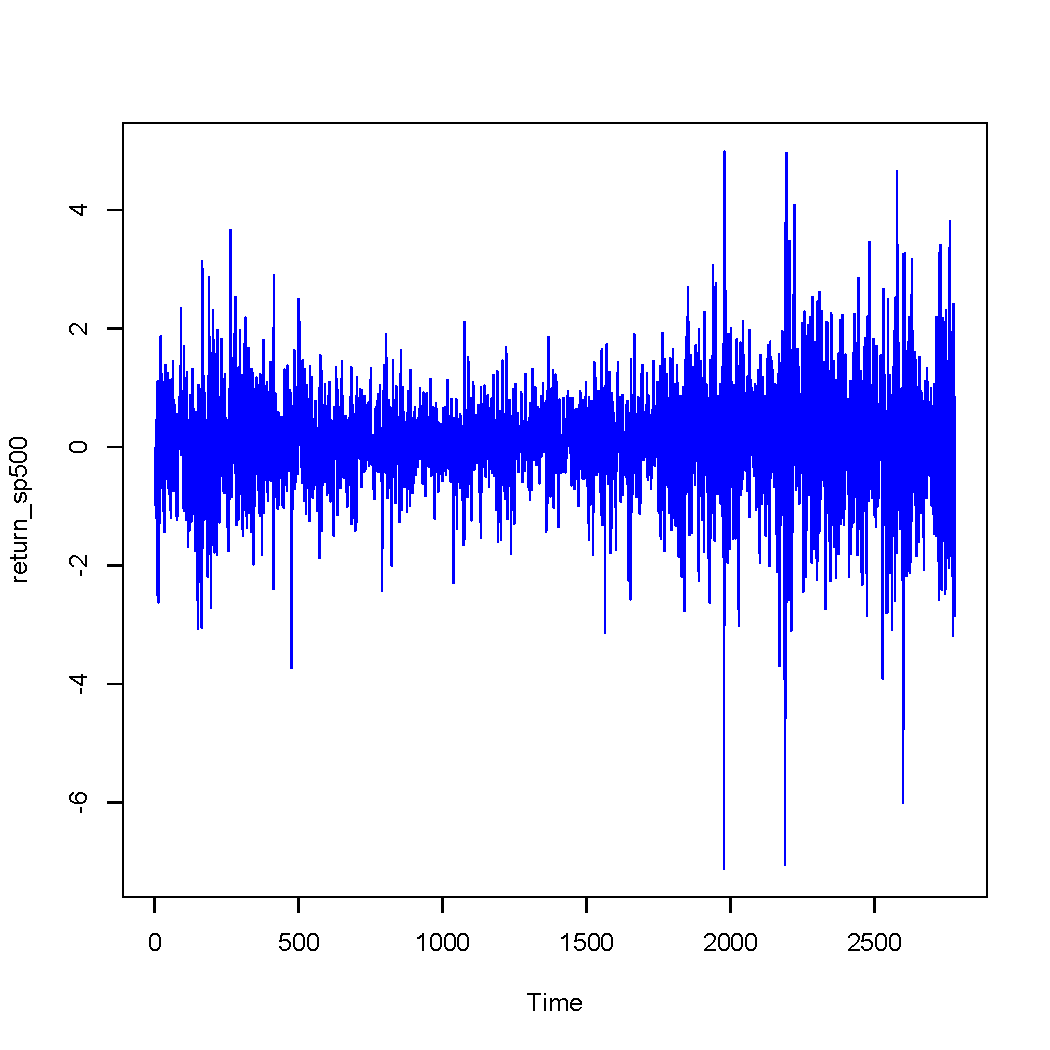
\includegraphics[width=0.5\textwidth,height=0.5\textheight]{R1.pdf}
\end{figure}
\end{example}
\end{frame}

\begin{frame}%
%EndExpansion

\frametitle{Continuous Distributions}

\begin{example}[cont'd]
Then, we analyze their distribution (e.g., some returns are more likely than some others?) via the histogram 
\begin{figure}[ptb]\centering
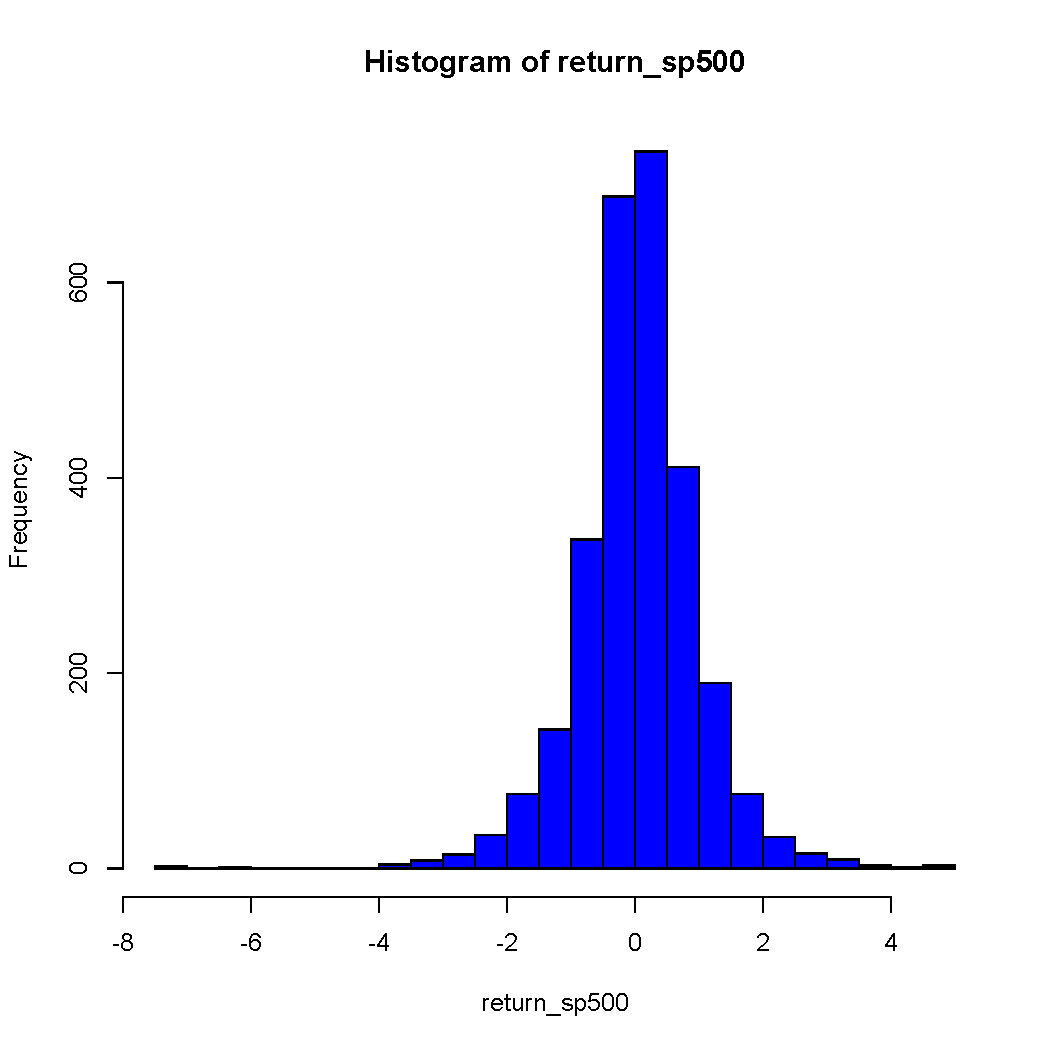
\includegraphics[width=0.65\textwidth,height=0.55\textheight]{sp_hist1.pdf}
\end{figure}
... with 30 bins ...
\end{example}
\end{frame}


\begin{frame}%
%EndExpansion

\frametitle{Continuous Distributions}

\begin{example}[cont'd]
%Then, we analyze their distribution via the histogram 
\begin{figure}[ptb]\centering
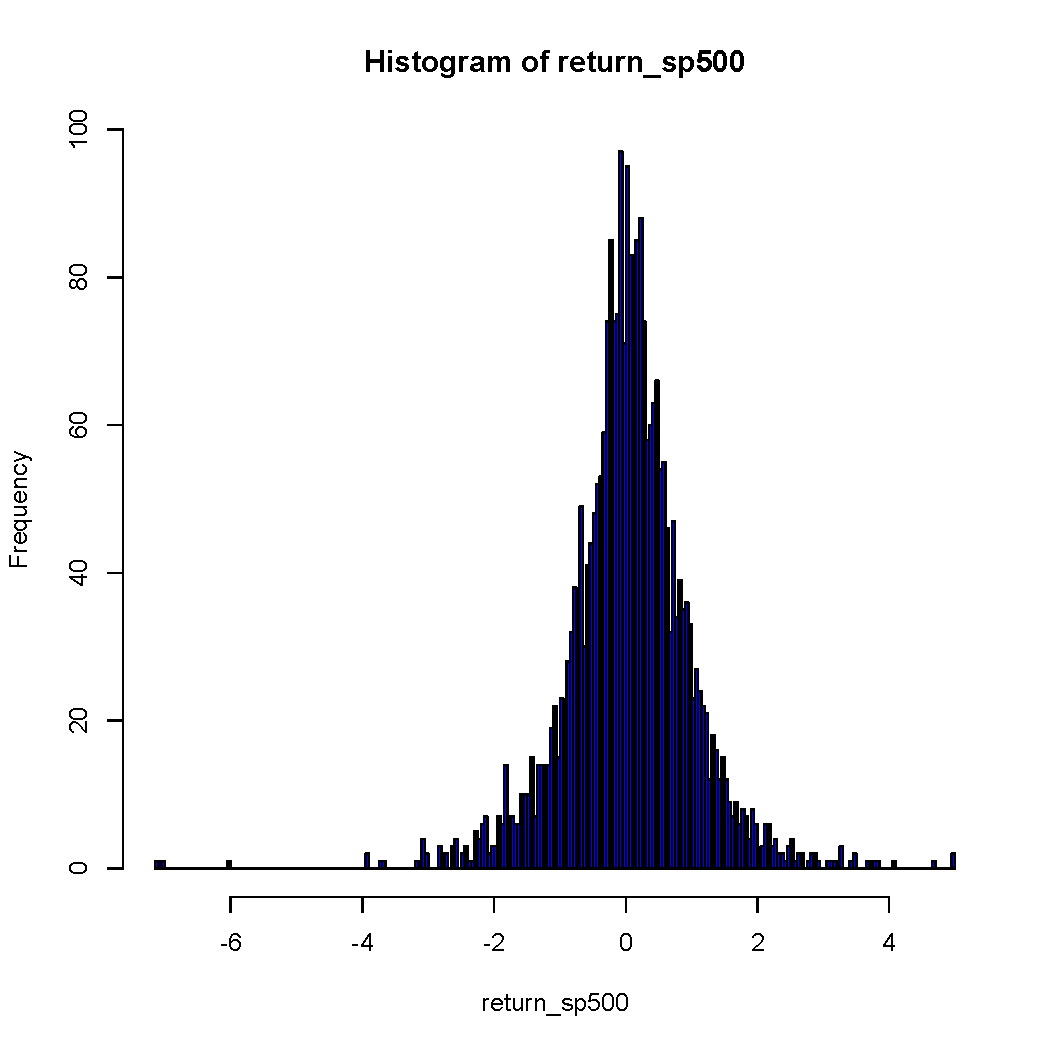
\includegraphics[width=0.65\textwidth,height=0.55\textheight]{sp_hist2.pdf}
\end{figure}
... with 300 bins ...
\end{example}
\end{frame}

\begin{frame}
\frametitle{Continuous Distributions}

\begin{example}[cont'd]
%Then, we analyze their distribution via the histogram 
\begin{figure}[ptb]\centering
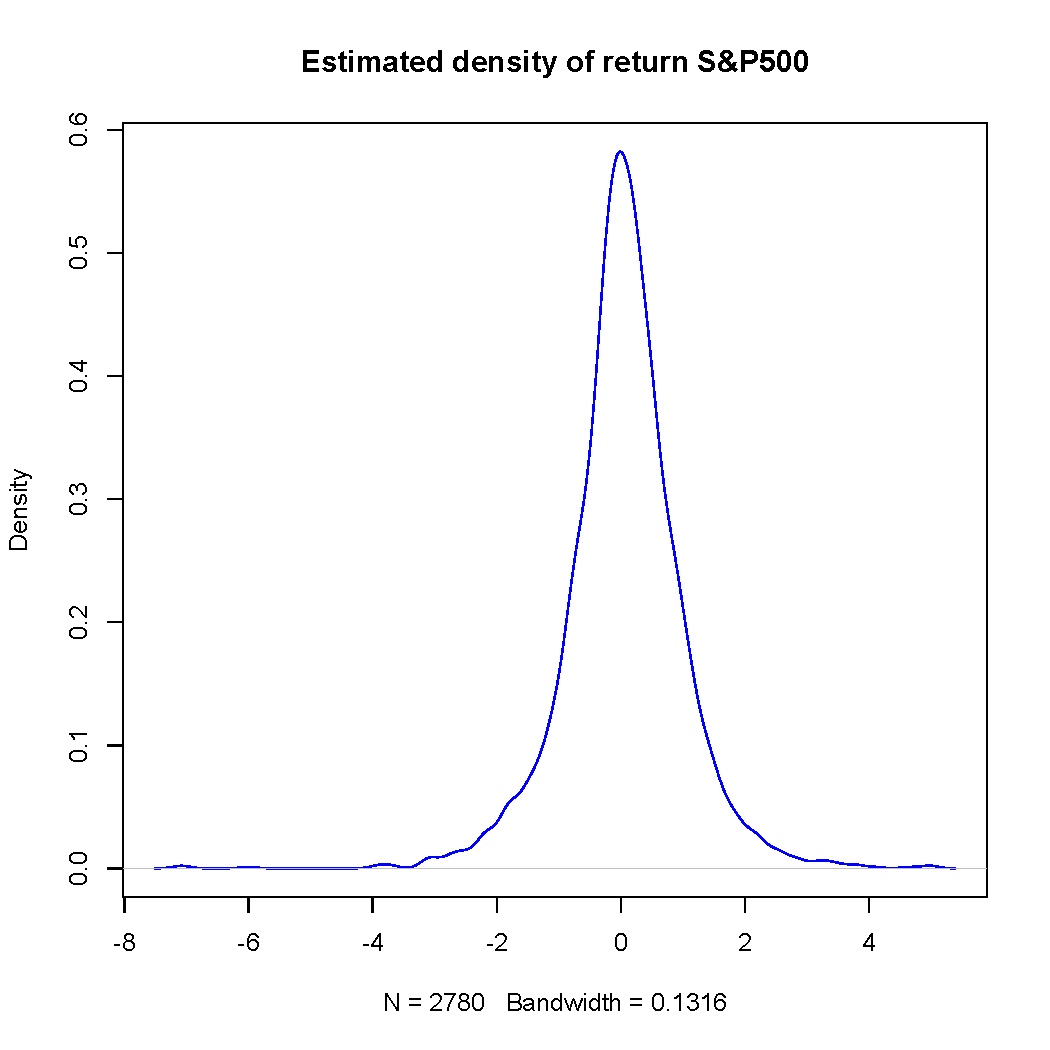
\includegraphics[width=0.65\textwidth,height=0.55\textheight]{R3_ks.pdf}
\end{figure}
... with an infinite number of bins (in fact, we are estimating a curve) 
\end{example}
\end{frame}


\begin{frame}%

\frametitle{Continuous Distributions}

\begin{example}[Cafeteria]
Let us consider a serious/significant issue: the arrivals to the cafeteria UniMail, from 10AM to 2PM
\begin{eqnarray*}
\mbox{relative freq}&=& \frac{\mbox{\# customers incoming }}{\mbox{ \# total of customers}}
\end{eqnarray*}

\begin{aes}
We want to study the distribution of this object over the considered time interval. E.g. we would like to know when the relative frequency has a pick...
\end{aes}

\end{example}
\end{frame}

\begin{frame}%
%EndExpansion

\frametitle{Continuous Distributions}
\begin{example}[cont'd]
\begin{figure}[ptb]\centering
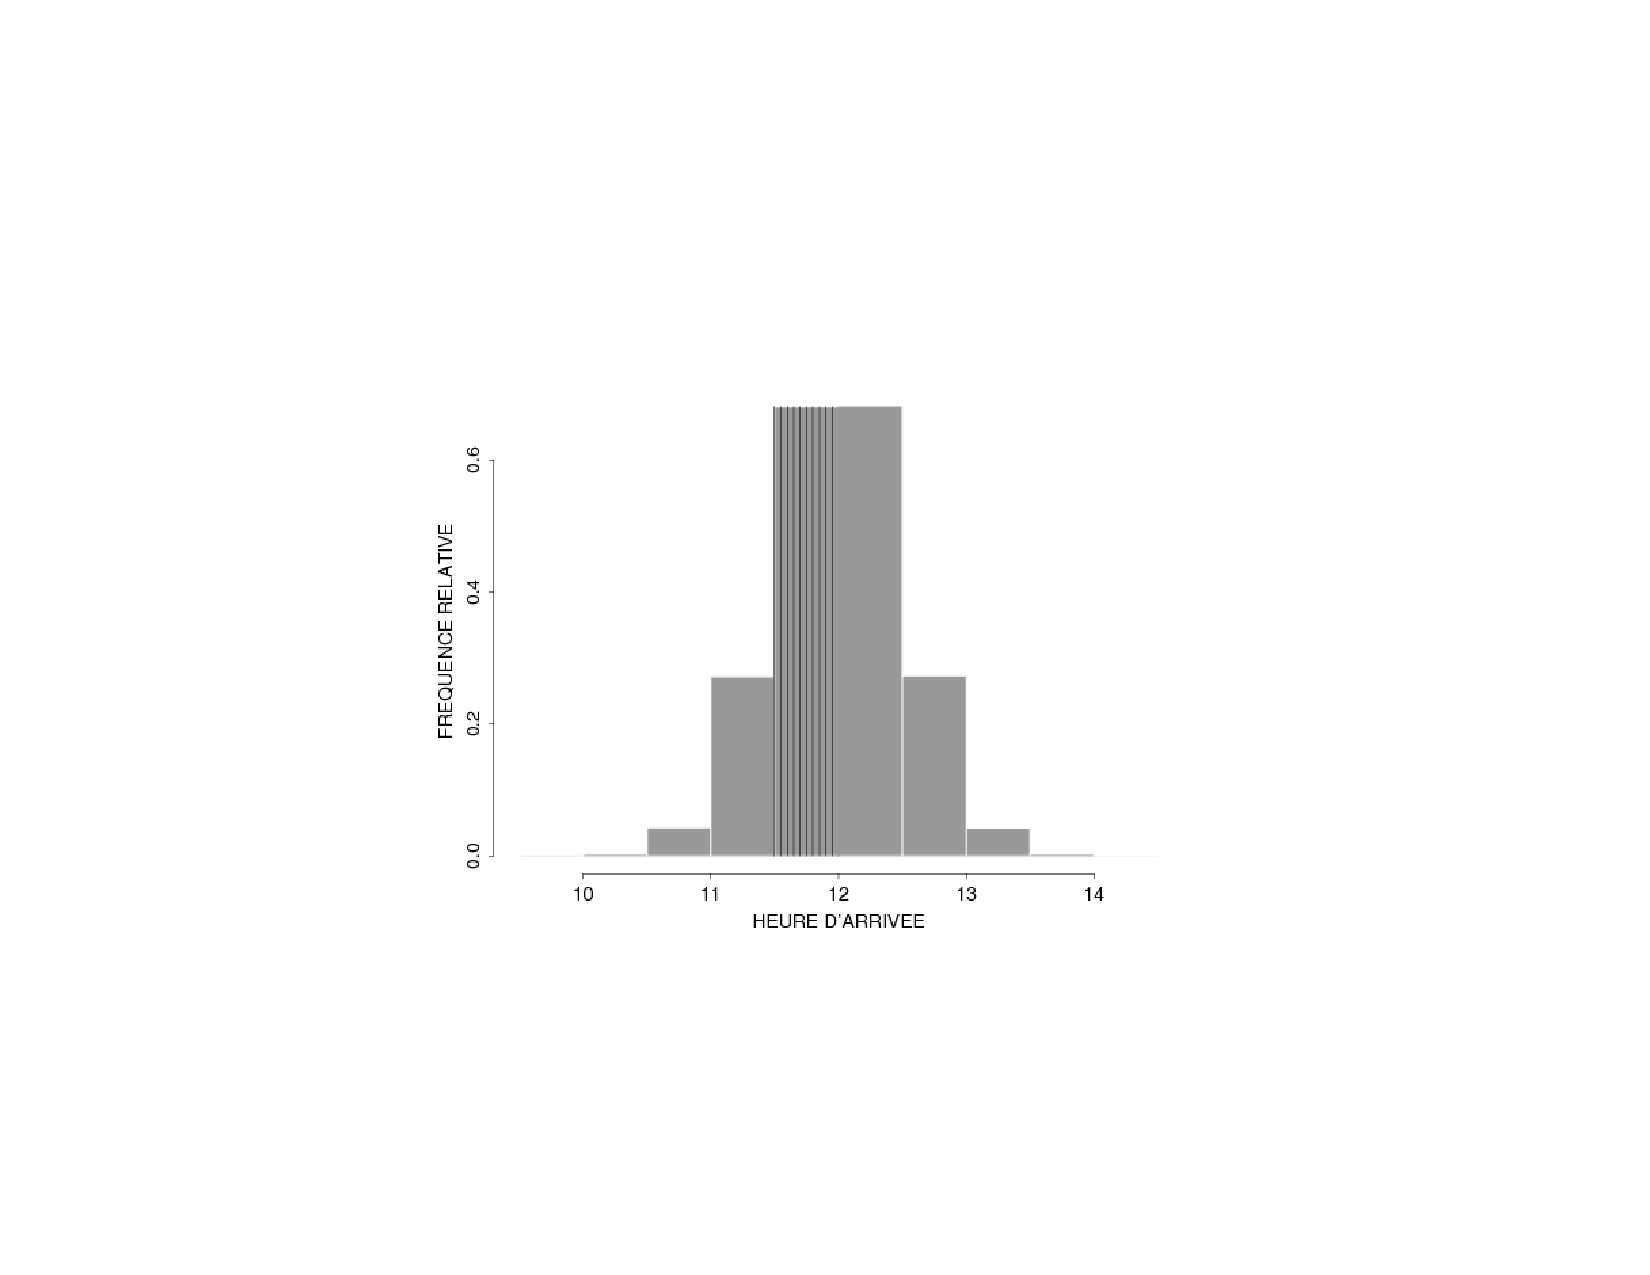
\includegraphics[width=0.75\textwidth,height=0.75\textheight]{hist1.pdf}
\end{figure}
\end{example}
\end{frame}

\begin{frame}%
%EndExpansion

\frametitle{Continuous Distributions}
\begin{example}[cont'd]
\begin{figure}[ptb]\centering
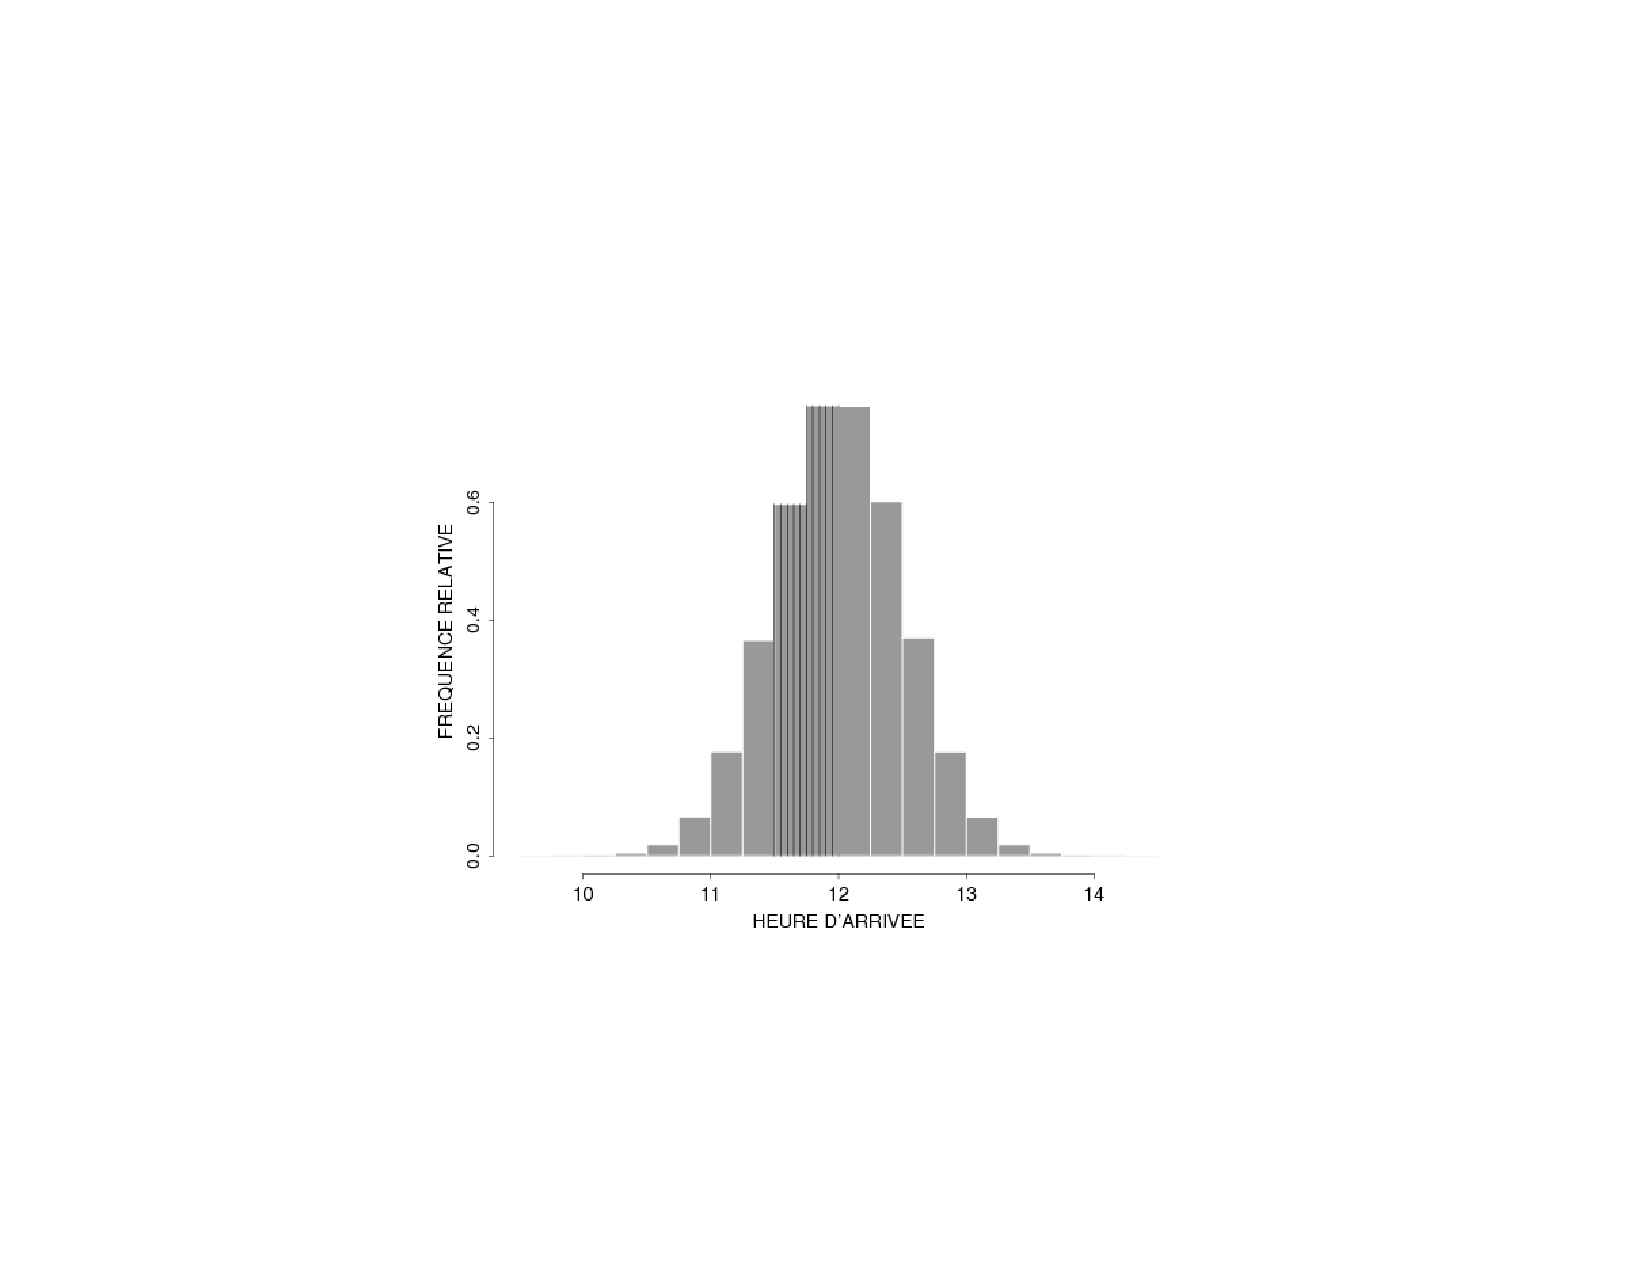
\includegraphics[width=0.75\textwidth,height=0.75\textheight]{hist2.pdf}
\end{figure}
\end{example}
\end{frame}

\begin{frame}%
%EndExpansion

\frametitle{Continuous Distributions}
\begin{example}[cont'd]
\begin{figure}
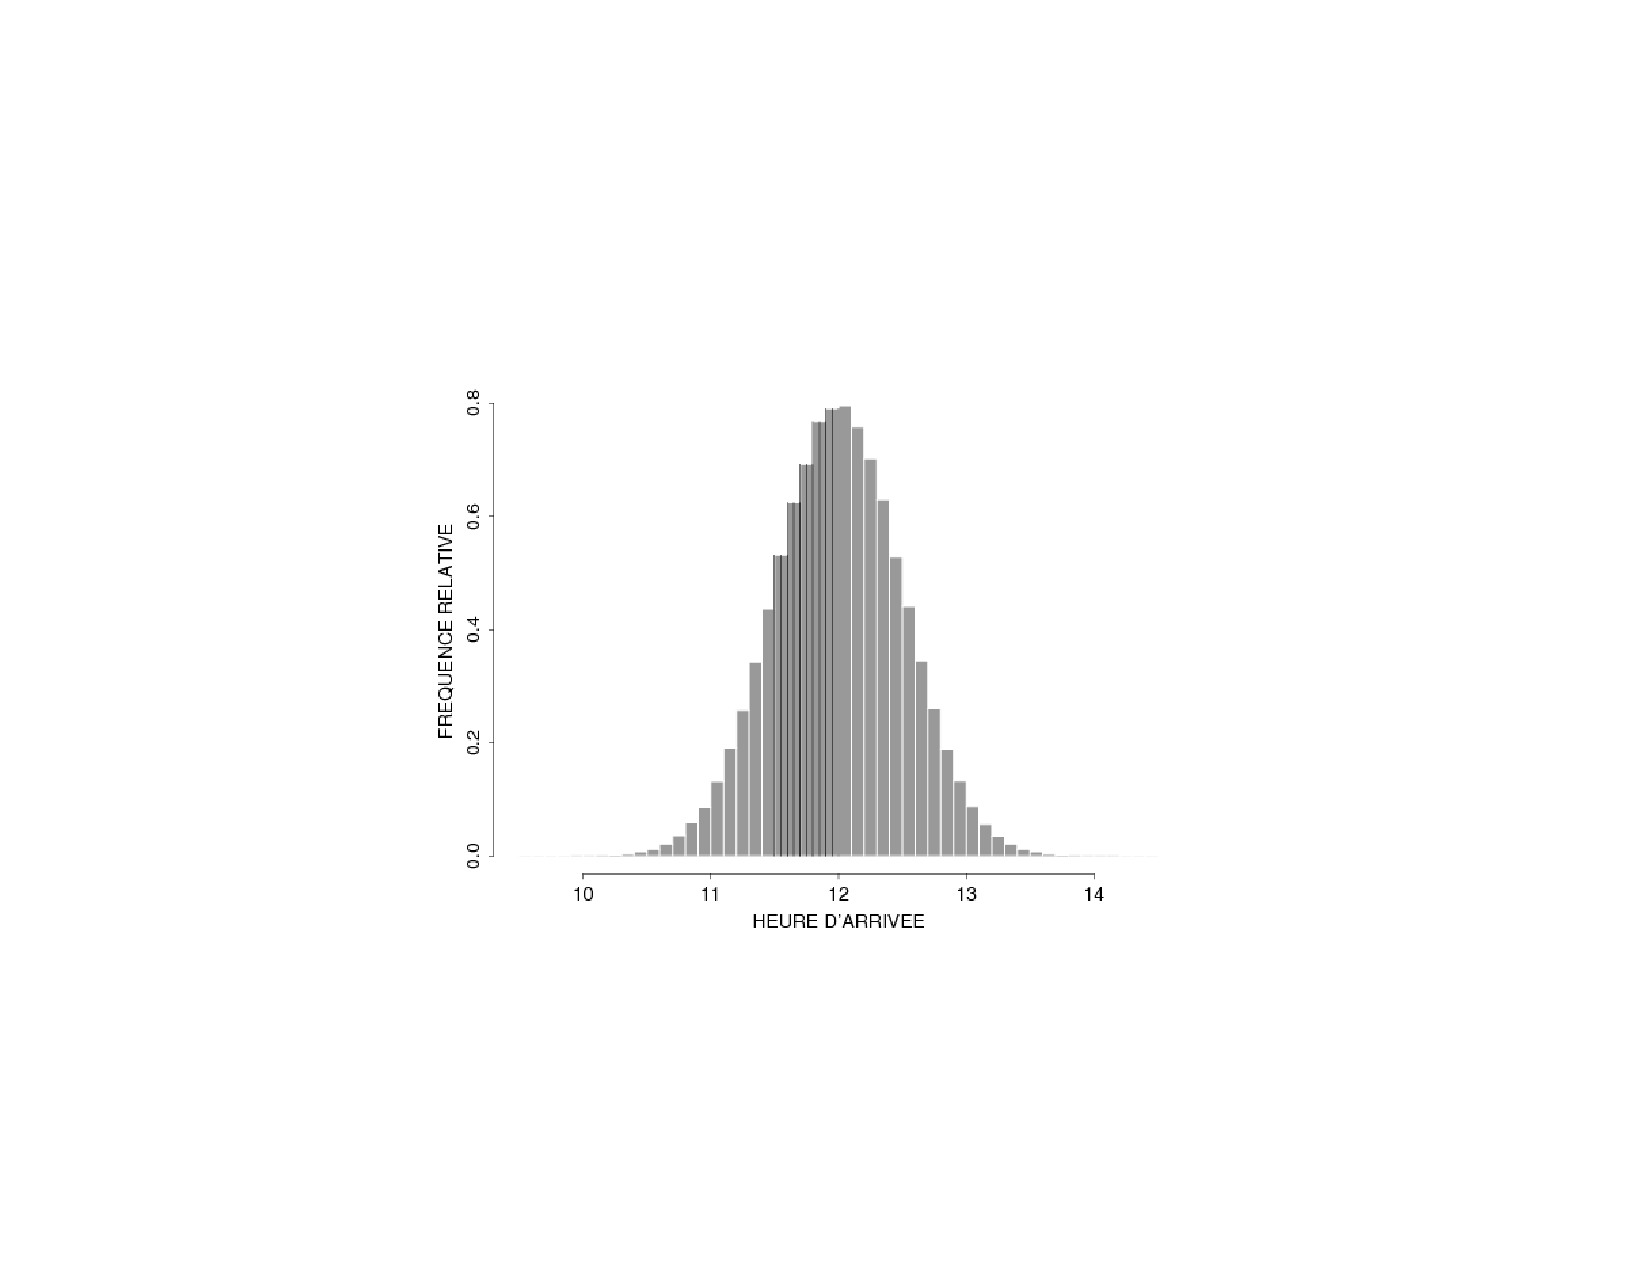
\includegraphics[width=0.75\textwidth,height=0.75\textheight]{hist3.pdf}
\end{figure}
\end{example}
\end{frame}


%\begin{frame}%
%%EndExpansion
%
%\frametitle{Continuous Distributions}
%
%\begin{centering}
%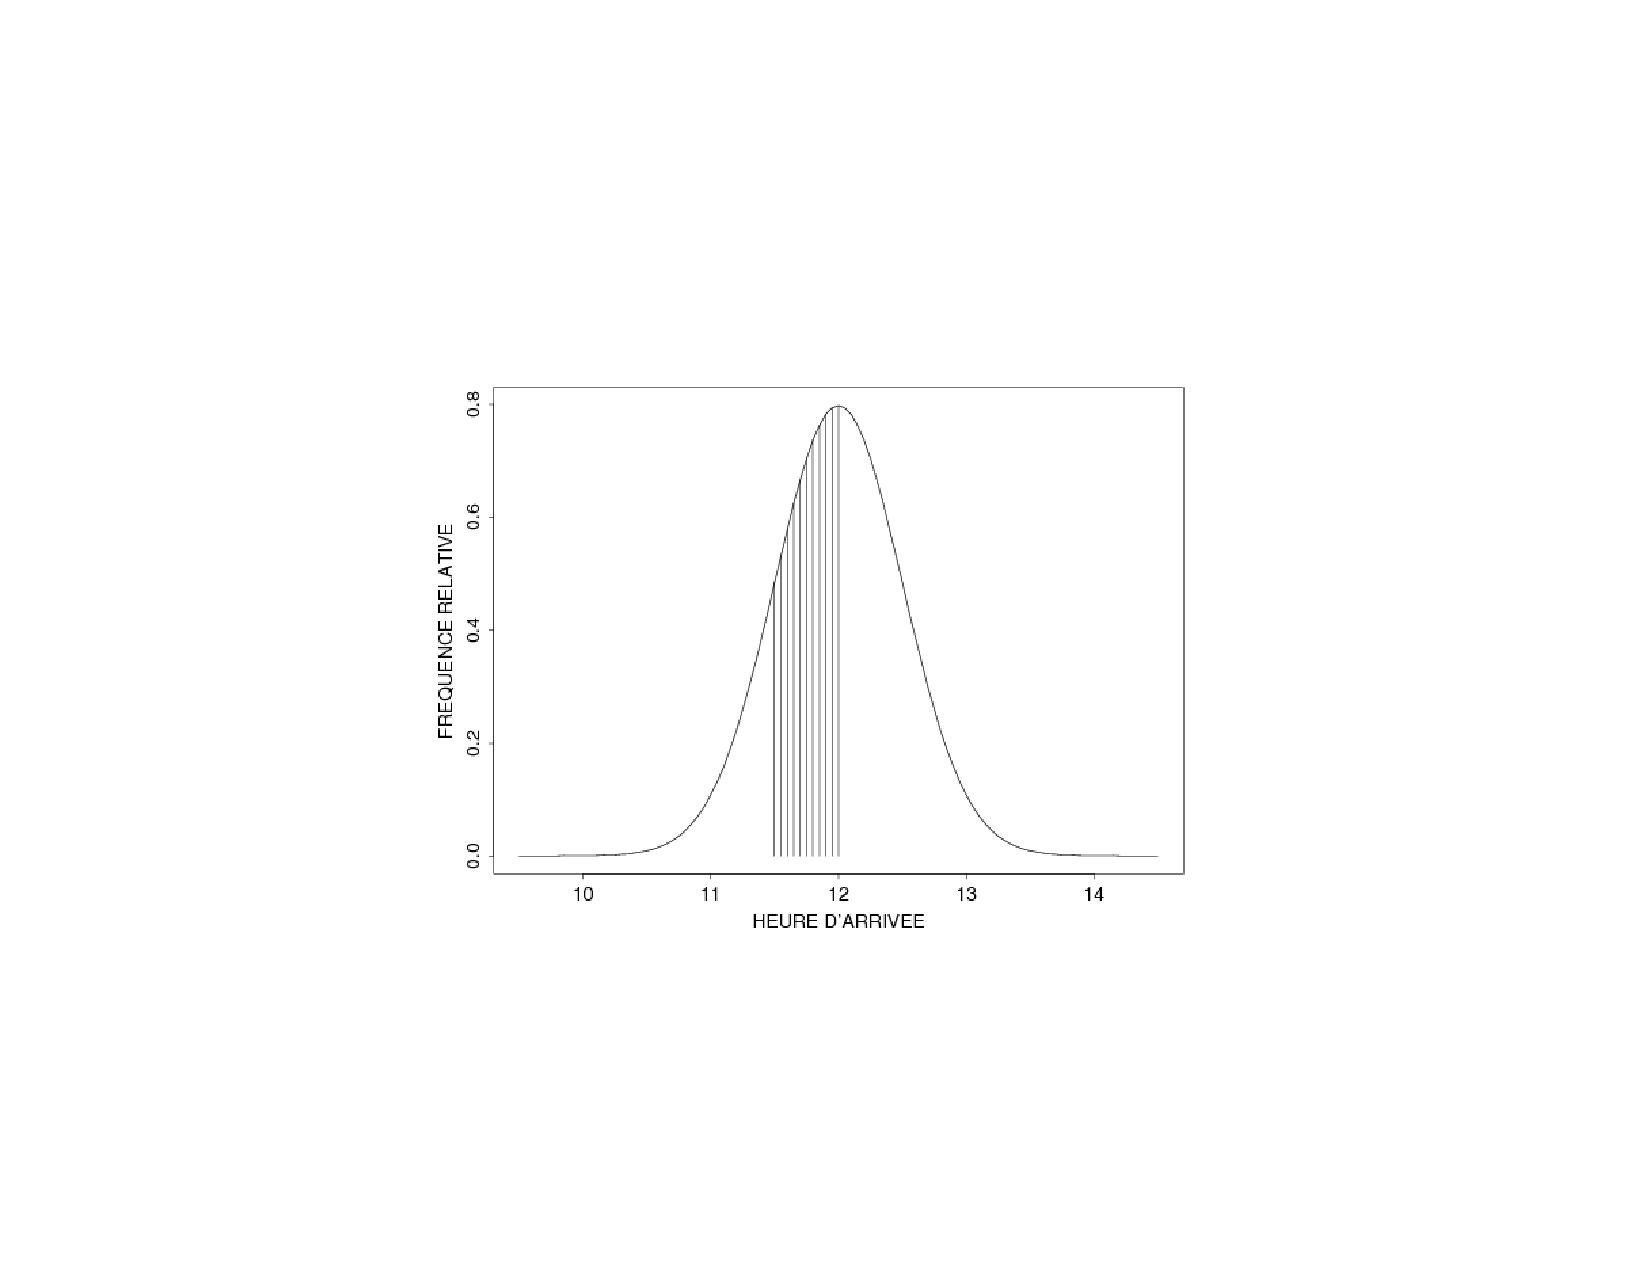
\includegraphics[width=0.5\textwidth,height=0.5\textheight]{hist4.pdf}
%\end{centering}
%\end{frame}
%


\begin{frame}%
\frametitle{Continuous Distributions}

The mentioned random variables provide two examples of a class of random variables which are different from what we have seen so far. 
Specifically, the examples emphasize that,
unlike discrete random variables, the considered variables are \textbf{continuous random variables}:
they can take any value in an interval. \\ \vspace{0.6cm}

This means we cannot simply \emph{list} all possible values of the
random variable, because there are (infinitely many) an uncountable number of possible outcomes that might occur. \\ \vspace{0.6cm}


 We construct a probability distribution by assigning a positive probability to each and every possible interval of values that can occur. This is done by defining what is called a \textbf{probability distribution function}. 

%TCIMACRO{\TeXButton{EndFrame}{\end{frame}}}%
%BeginExpansion
\end{frame}%
%EndExpansion


\begin{frame}%
\frametitle{Continuous Distributions}
So, graphically, we have \\ \vspace{0.5cm}
\begin{figure}
\hspace{1cm} Discrete \hspace{3cm} Continuous\\
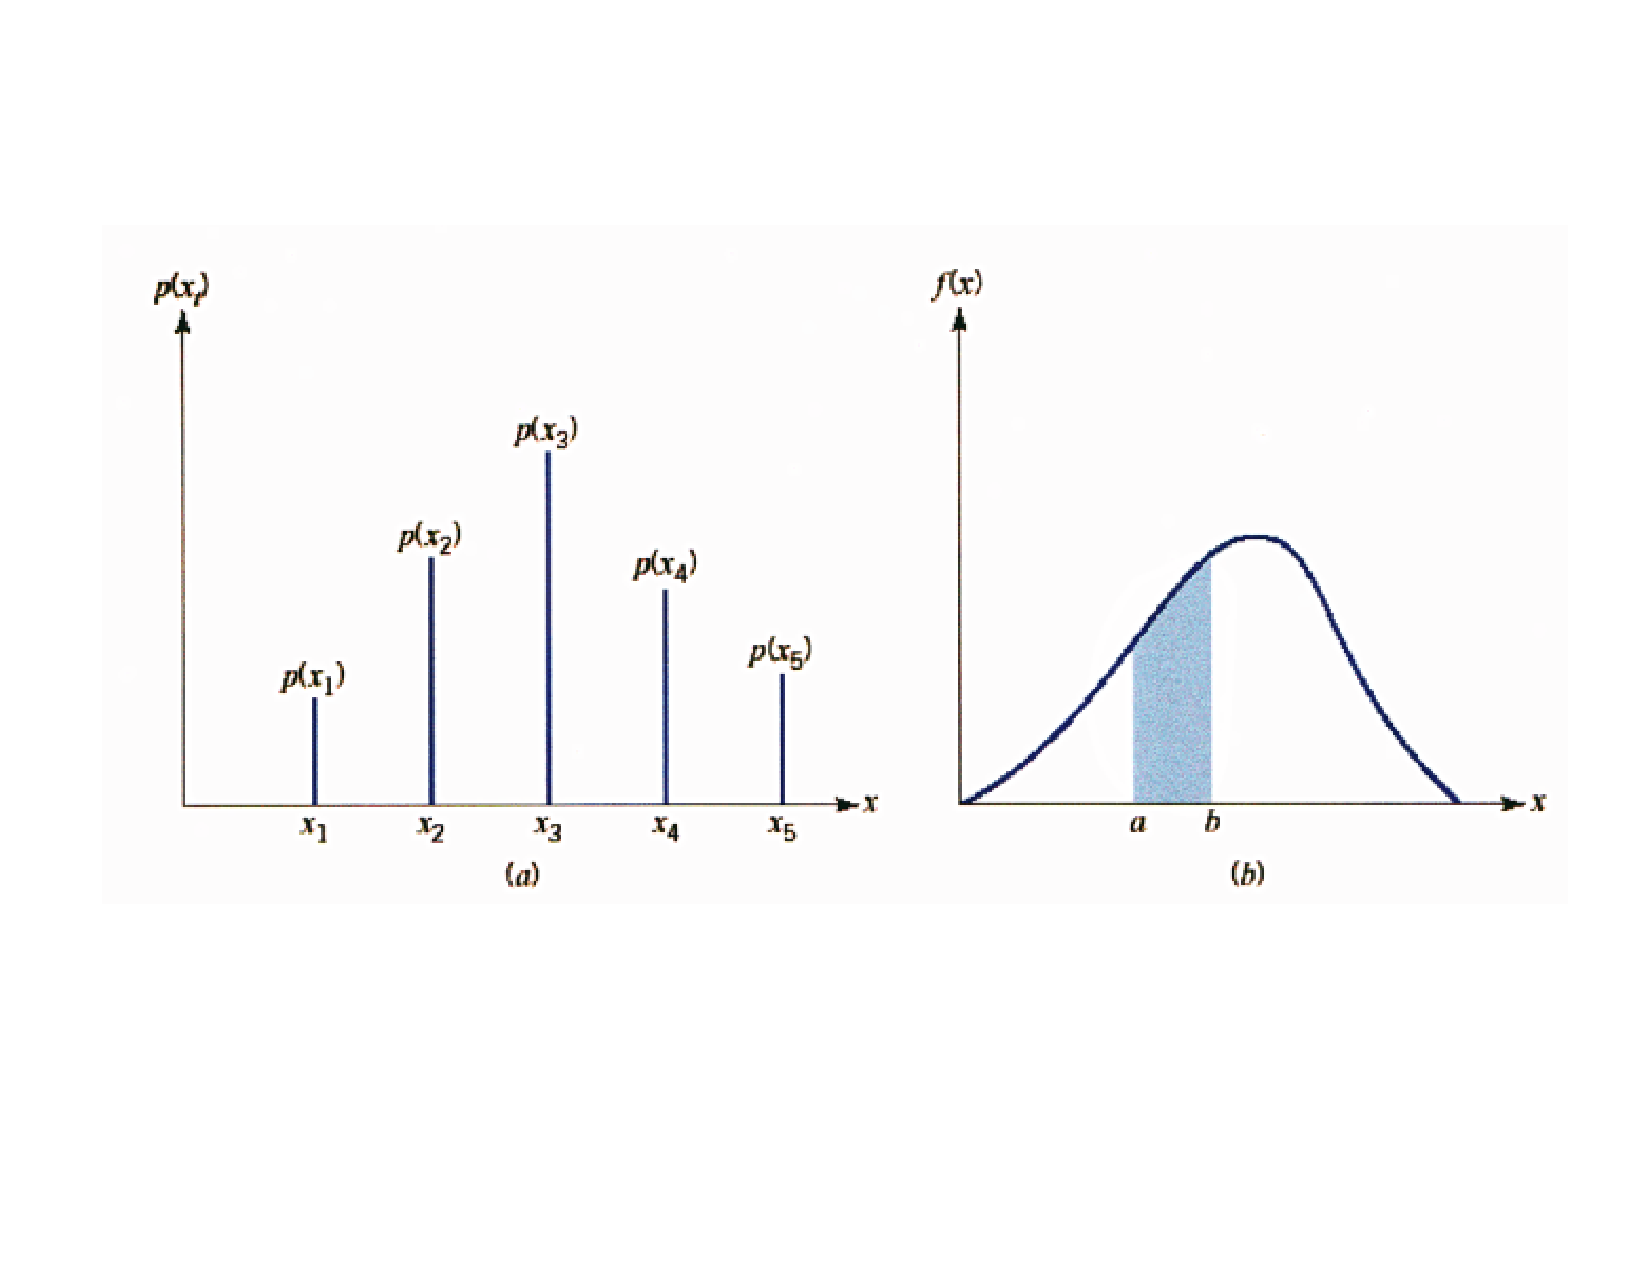
\includegraphics[width=0.75\textwidth,height=0.5\textheight]{discr_vs_cont.pdf}
\end{figure}

\end{frame}%


%TCIMACRO{\TeXButton{BeginFrame}{\begin{frame}}}%
%BeginExpansion
\begin{frame}%
%EndExpansion

\frametitle{Cumulative Distribution Function (CDF)}

\begin{definition}
 Let $X$ be a continuous random variable and let $x\in \mathbb{R}$, here $x$ denotes any number somewhere on the real line $\mathbb{R}=(-\infty,\infty)$. The Probability Distribution Function (synonymously, the Cumulative Distribution Function
\color{red}%
CDF%
\color{black}) of $X$ at the point $x$ is a continuous function
\color{red}%
$F_{X}\left( x\right) $
\color{black}
defined such that
\begin{stepenumerate} \vspace{0.3cm}
\item $\color{red}F_{X}\left( -\infty\right)\color{black}=0$ and $\color{red}F_{X}\left(\infty\right)\color{black}=1$,\vspace{0.3cm}
\item $0\leq \color{red}F_{X}\left( x\right)\color{black} \leq 1$ for all $x\in \mathbb{R}$ and\vspace{0.3cm}
\item the function is monotonically non-decreasing in $x$ and the value $\color{red}F_{X}\left( x\right)\color{black} $ yields the probability that $X$ lies in the interval $(-\infty,x]$, i.e.%
$$
\color{red} F_{X}\left( x\right)\color{black}\geq \color{red}F_{X}\left( x'\right)\color{black}\quad\mbox{for all}\quad x>x'
$$
and
$$
\Pr \left( X\leq x\right)=\color{red}F_{X}\left( x\right) \color{black}.
$$
\end{stepenumerate}
\end{definition}
\end{frame}%

\begin{frame}%

\frametitle{Cumulative Distribution Function (CDF)}

Let $X$ be a random variable taking values in the interval $(a,b]$ since
\vspace{0.75cm}

\begin{stepitemize}
\item $\color{red}F_{X}\left( x\right)\color{black} $ is zero for all $x<a$ \vspace{0.25cm}
\item $0<\color{red}F_{X}\left( x\right)\color{black}<1 $ for all $x$ in $(a,b)$ and \vspace{0.25cm}
\item $\color{red}F_{X}\left( x\right)\color{black}=1 $ for all $x\geq b$.
\end{stepitemize}

\vspace{0.75cm}

Then, the Probability Density Function (\color{blue}pdf\color{black}) of $X$ at the point $x$ is defined as
\begin{equation*}
\color{blue}{f_{X}\left( x\right) =\frac{d\color{red}F_{X}(x)\color{black}}{dx}}\,.
\end{equation*}%

\end{frame}%

%EndExpansion

%TCIMACRO{\TeXButton{EndFrame}{\end{frame}}}%
%BeginExpansion
\begin{frame}%
%EndExpansion

\frametitle{Probability Density Function (pdf)}
 
 ... an illustration ...
 
\begin{figure}[ptb]\centering
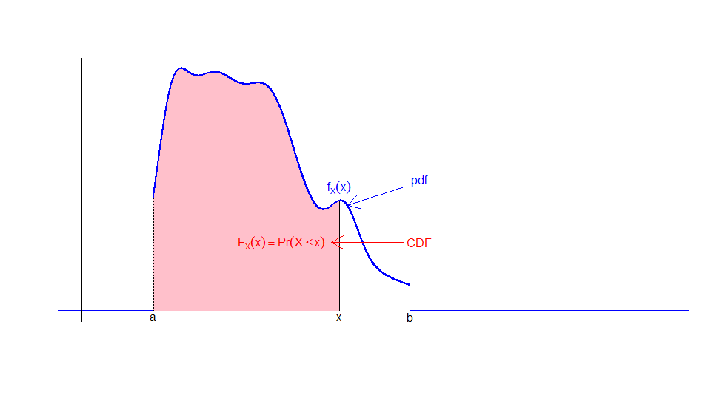
\includegraphics[width=0.95\textwidth,height=0.75\textheight]{generic_CDF2.pdf}%
\end{figure}%

%\begin{stepitemize}
%\item Let $X$ be a continuous random variable with continuous CDF $F_{X}\left( x\right)$.
%
%\item Then the Probability Density Function (%
%%TCIMACRO{\TeXButton{blue}{\color{blue}}}%
%%BeginExpansion
%\color{blue}%
%%EndExpansion
%PDF%
%%TCIMACRO{\TeXButton{black}{\color{black}}}%
%%BeginExpansion
%\color{black}%
%%EndExpansion
%) of $X$ at the point $x$ is defined as
%\begin{equation*}
%\color{blue}{f_{X}\left( x\right) =\frac{dF_{X}(x)}{dx}}\,.
%\end{equation*}%
%%for all $x\in \mathbb{R}$.
%\item For the illustrated CDF we have:
%\end{stepitemize}
%%TCIMACRO{%
%%\FRAME{ftbpF}{4.67in}{2.5624in}{0pt}{}{}{generic_pdf.bmp}{%
%%\special{language "Scientific Word";type "GRAPHIC";maintain-aspect-ratio TRUE;display "USEDEF";valid_file "F";width 4.67in;height 2.5624in;depth 0pt;original-width 13.4859in;original-height 7.389in;cropleft "0";croptop "1";cropright "1";cropbottom "0";filename 'generic_pdf.bmp';file-properties "XNPEU";}}}%
%%BeginExpansion
%\begin{figure}[ptb]\centering
%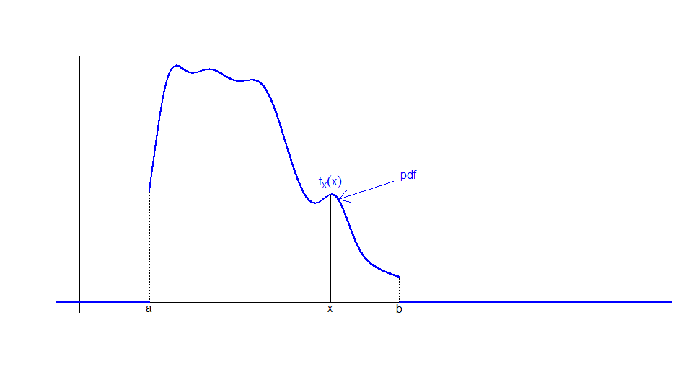
\includegraphics[width=0.95\textwidth]{generic_pdf__1.pdf}%
%\end{figure}%
%EndExpansion

%TCIMACRO{\TeXButton{EndFrame}{\end{frame}}}%
%BeginExpansion
\end{frame}%


\begin{frame}%
%EndExpansion

\frametitle{Probability Density Function (pdf)}
 
 ... \textit{repetita juvant} ...
 
\begin{figure}[ptb]\centering
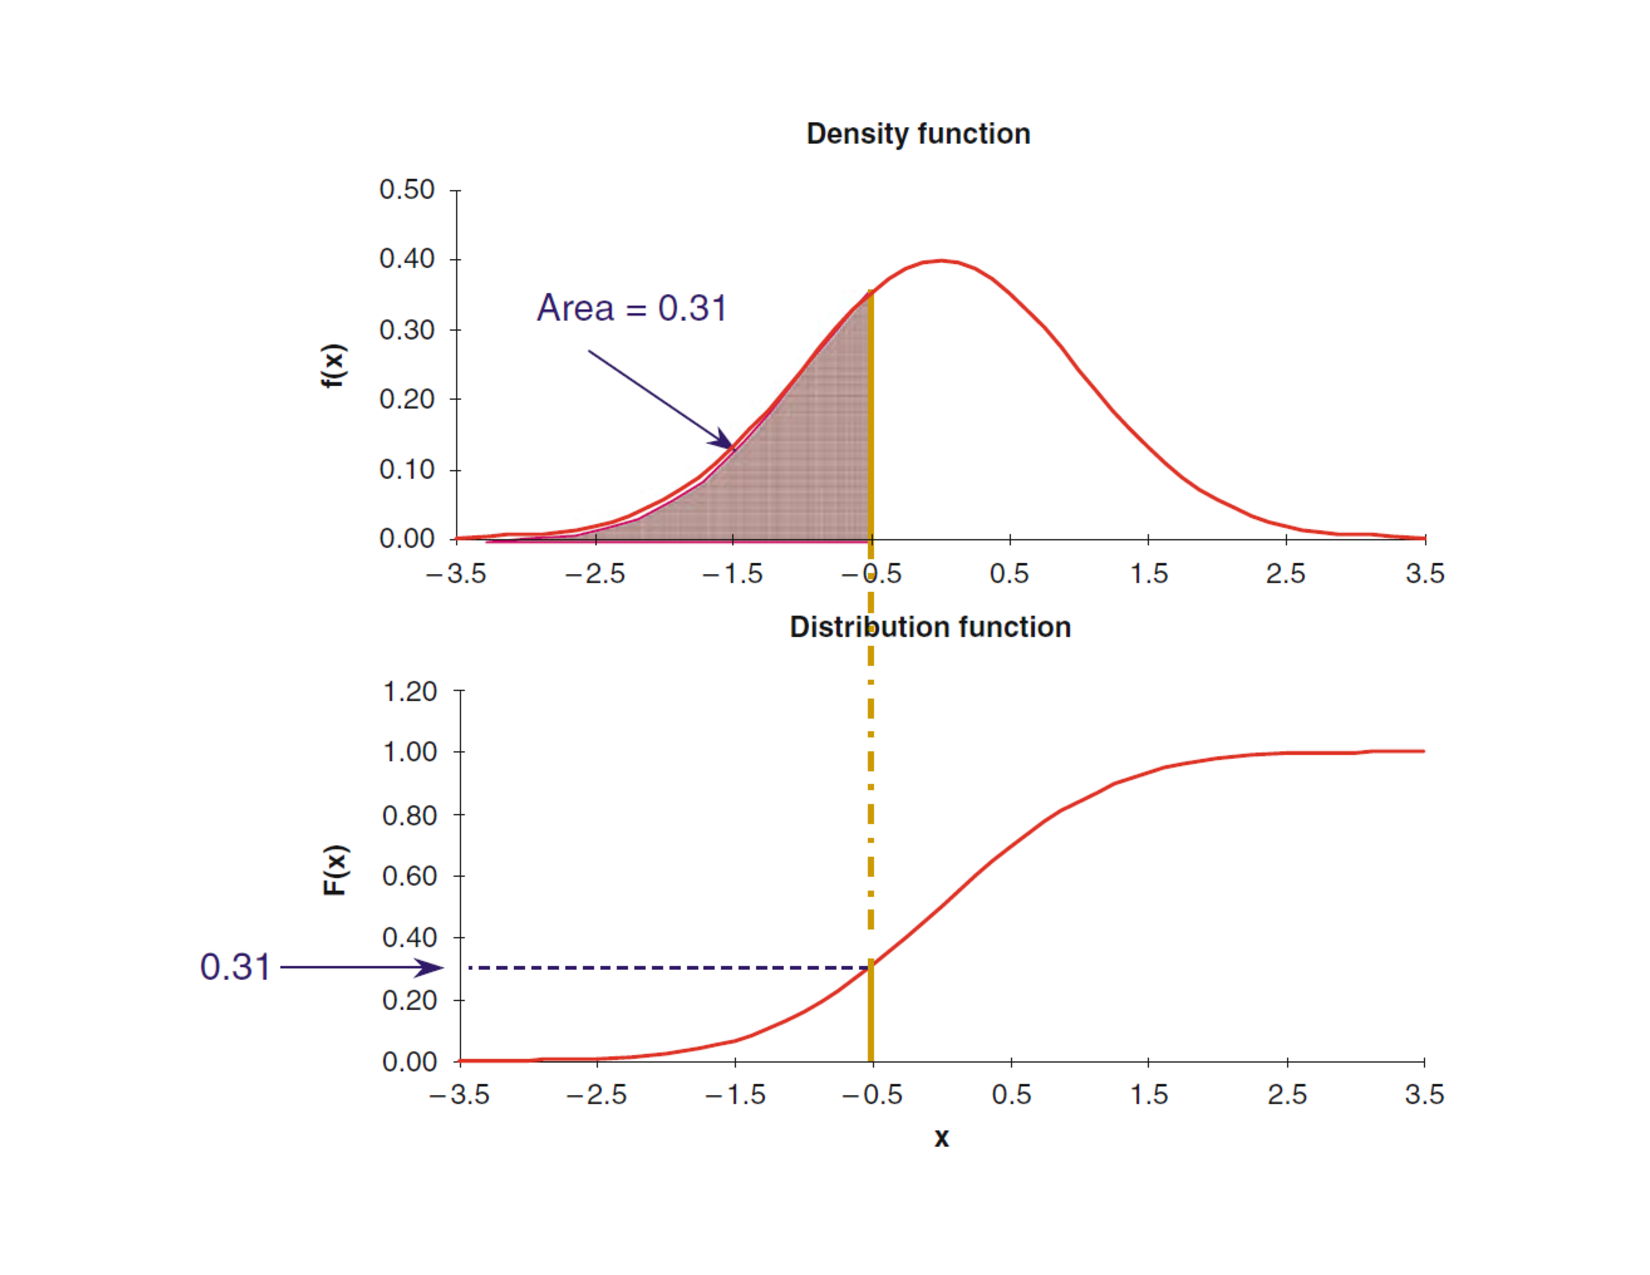
\includegraphics[width=0.7\textwidth,height=0.65\textheight]{Diego_F.pdf}%
\end{figure}%

\end{frame}

%EndExpansion
%
%\begin{frame}
%\frametitle{Probability Density Function (pdf)}
% 
% ... and a cartoon ...
% 
%\begin{figure}[ptb]\centering
%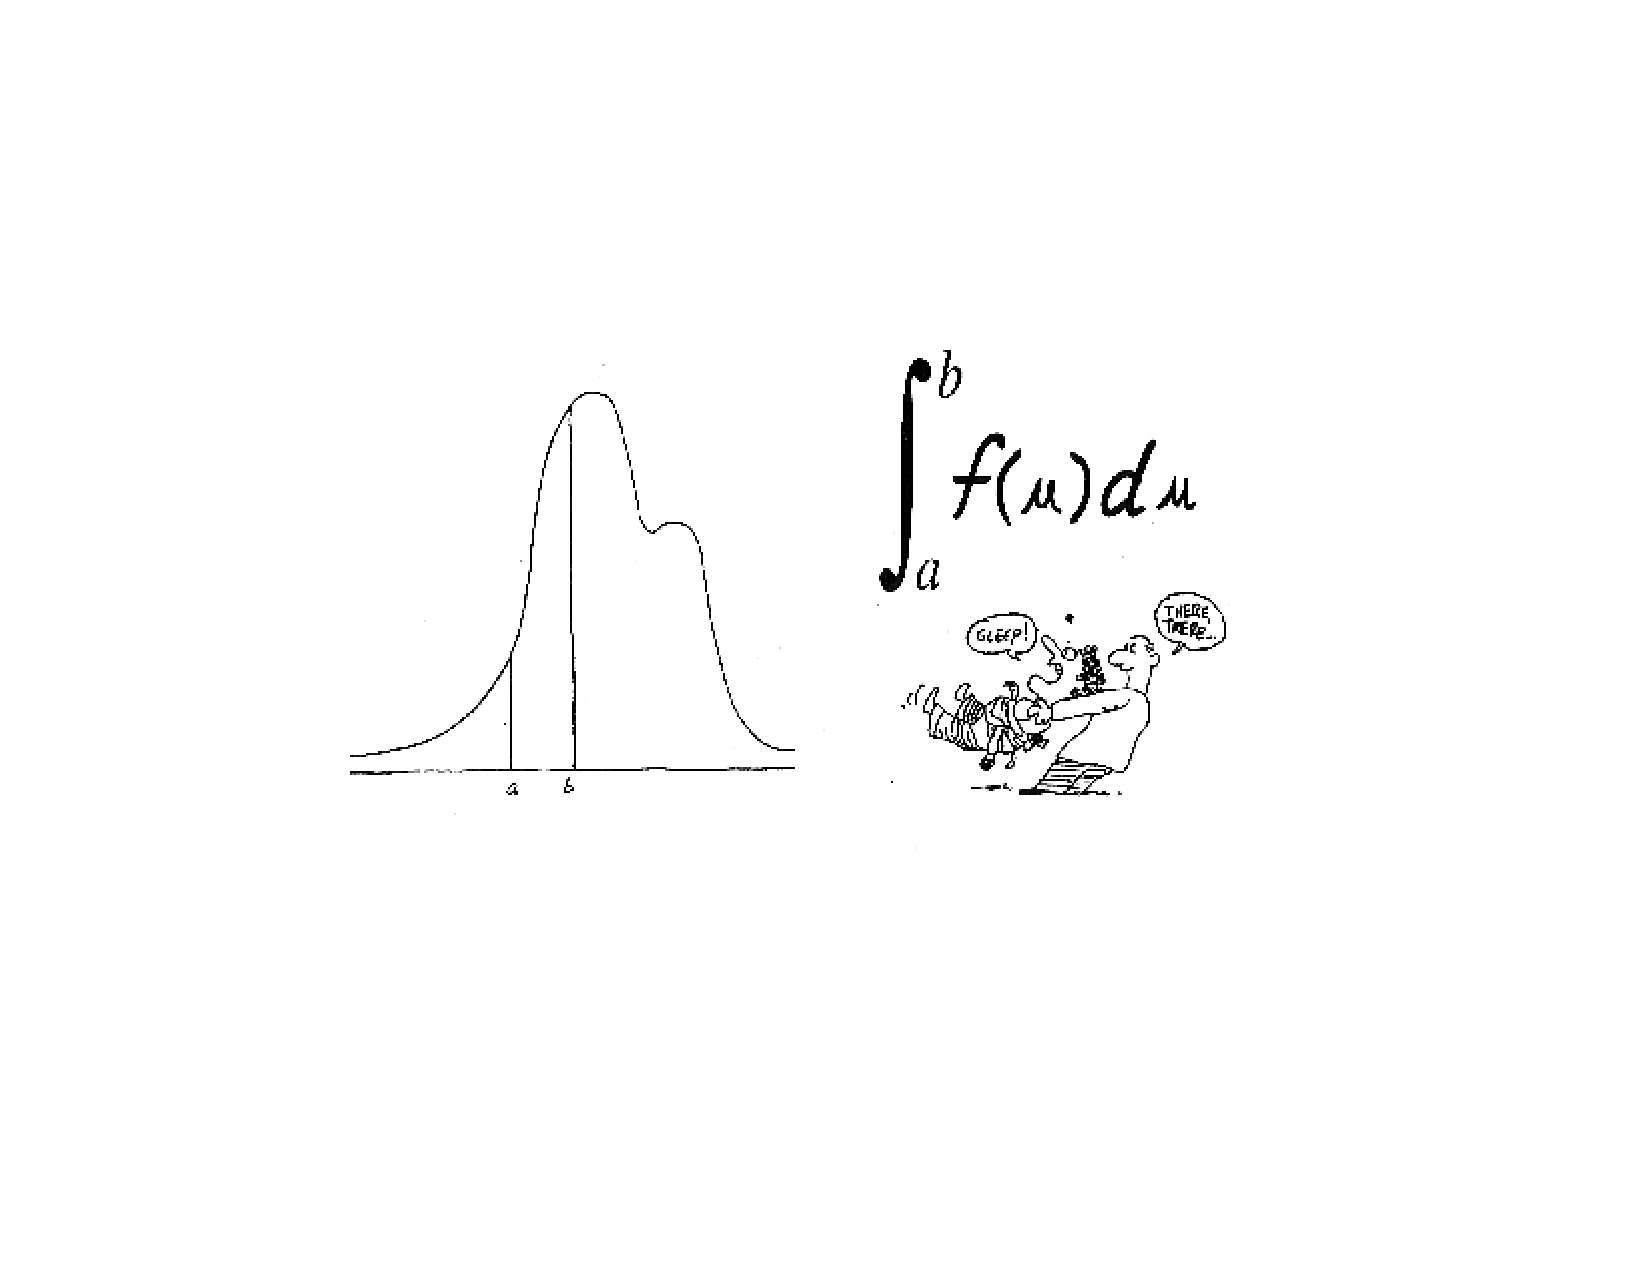
\includegraphics[natheight=7.6in, natwidth=13.4859in, height=2.4in, width=4.67in]{aaa.pdf}%
%\end{figure}%
%
%\end{frame}

%TCIMACRO{\TeXButton{EndFrame}{\end{frame}}}%
%BeginExpansion
\begin{frame}%
%EndExpansion

\frametitle{Probability Density Function (pdf)}

In the illustration $X$ is a random variable taking values in the interval $(a,b]$, and the pdf $f_{X}\left( x\right) $ is non-zero only in $(a,b)$. More generally we have, for a variable taking values on the whole real line ($\mathbb{R}$) \vspace{0.3cm}
%by the \textbf{\emph{fundamental theorem of integral calculus}}:%
%\begin{equation*}
%F_{X}(x)=\int_{-\infty}^{x}f_{X}\left( t\right) dt
%\end{equation*}
%for any value of $x\in \mathbb{R}$. Thus we  deduce that the PDF $f_{X}\left( x\right) $ is such that
%\begin{stepitemize}
%\item $f_{X}\left( x\right) \geq 0$ for all $x\in \mathbb{R}$
%\item The total area under the curve $f_{X}\left( x\right) $ is 1, i.e. $
%\int_{-\infty }^{\infty }f_{X}\left( x\right) dx=1.$
%\item Note that for some intervals of the real line, we can have $f_{X}\left( x\right) =0$.
%\end{stepitemize}
%Moreover (see the previous graphical illustration), recall that:
\begin{stepitemize}
\item the \textbf{\emph{fundamental theorem of integral calculus}} yields
\color{red}
$$F_{X}\left( x\right) =\Pr \left( X\leq x\right) =\int_{-\infty}^{x}\color{blue}f_{X}\left(
t\right)\color{red} dt,$$%
\color{black}
the area under the CDF between $-\infty$ and $x$ \vspace{0.3cm}

\item or in terms of derivative
$$
\color{blue}f_{X}\left( x\right) \color{black} = \frac{d\color{red}F_{X}(x) \color{black}}{\color{black} dx}
$$ 
for all $x$, the derivative of the CDF\footnote{From now on, no more red and blue color}.
\end{stepitemize}




\end{frame}%

\begin{frame}%

\frametitle{Probability Density Function (pdf)}

Most of the pdfs that we are going to consider are bell-shaped. So, typically, we will have 
\begin{figure}[h]
\begin{center}
\begin{tabular}{cc}
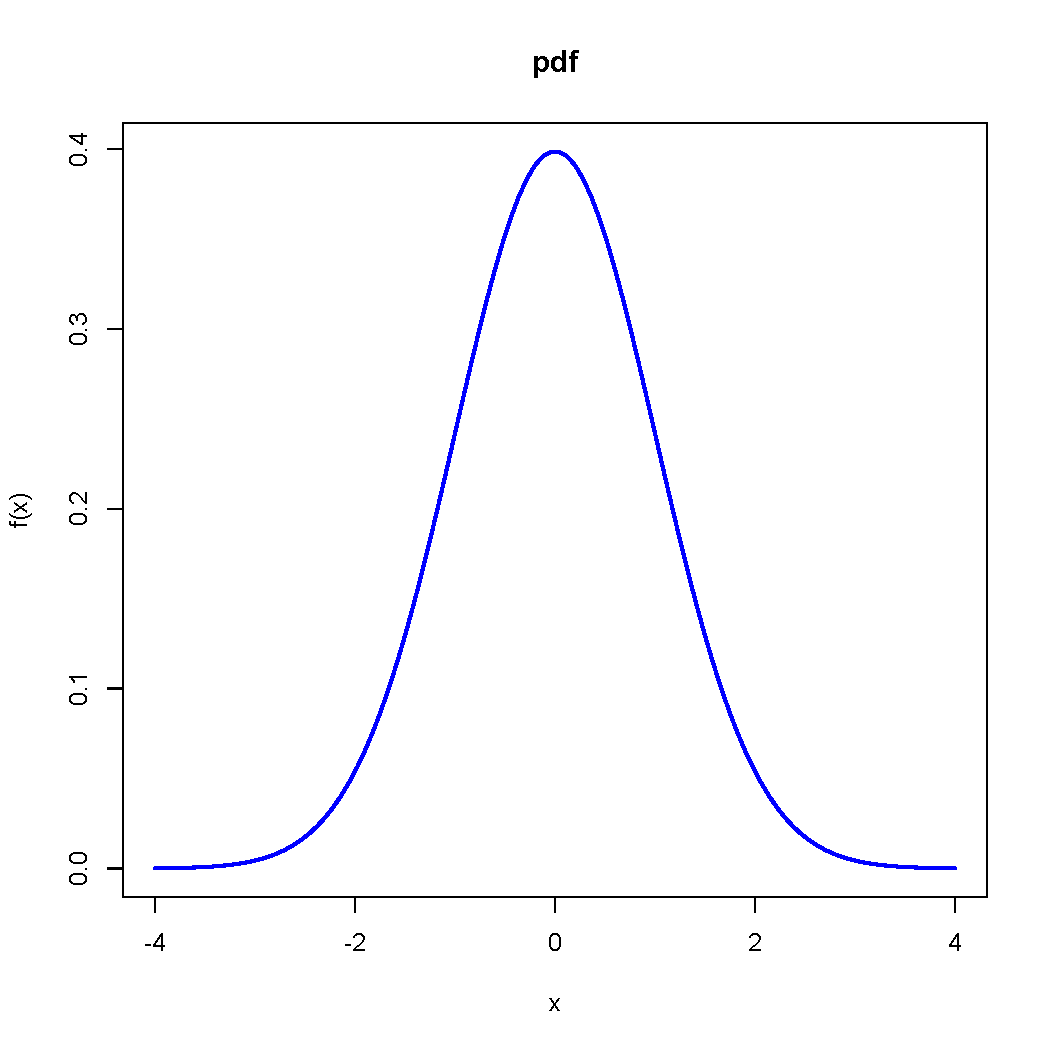
\includegraphics[width=5cm, height=5.cm]{R_bell_pdf} & 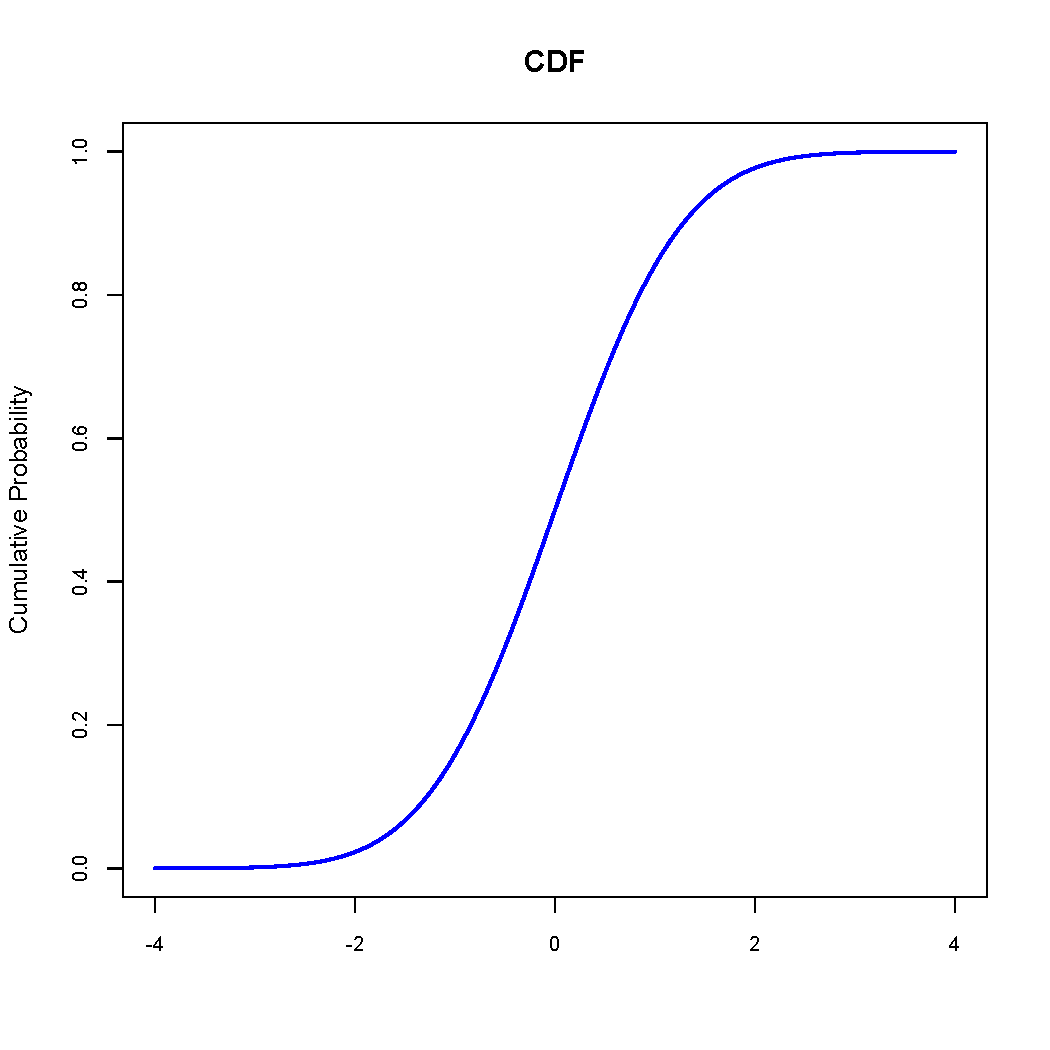
\includegraphics[width=5cm, height=5cm]{R_bell_CDF.pdf} \\
\end{tabular}
\end{center}
\par
\end{figure}


\end{frame}%


\begin{frame}%

\frametitle{The mean (or expected) value}

For \textbf{discrete} random variables, we use summation:%
\begin{equation*}
E\left[ X\right] =\sum_{i}x_{i}p_{i}
\end{equation*}

\begin{stepitemize}
\item the mean (or expected) value of a discrete random variable $X$

\item is found by summing the product of $x_{i}$ and $p_{i}=\Pr (X=x_{i})$,

\item for each possible value $x_{i}$
\end{stepitemize}

\vspace{0.4cm}

For \textbf{continuous} random variables, we use itegration:%
\begin{equation*}
E\left[ X\right] =\int_{a}^{b}x\,f_{X}\left( x\right) dx
\end{equation*}

\begin{stepitemize}
\item the mean (or expected) value of the continuous random variable $X$

\item is found by integrating the product of $x$ and its \textbf{pdf }$%
f_{X}\left( x\right) $

\item over the range of possible values of $x$
\end{stepitemize}

\end{frame}%

\begin{frame}%
\frametitle{The Variance}

Recall that, for \textbf{discrete} random variables, we defined the variance as: \vspace{0.5cm}
\begin{equation*}
Var\left( X\right) =\sum_{i}\left( x_{i}-E\left[ X\right] \right) ^{2}\Pr
\left( X=x_{i}\right)
\end{equation*}

\vspace{1cm}

Similarly, for \textbf{continuous} random variables, we use integration\footnote{Intuitively, we replace the sum ($\sum$) by its continuous counterpart, namely the integral ($\int$). }:
\vspace{0.5cm}

\begin{equation*}
Var\left( X\right) =\int_{a}^{b}\left( x-E\left[ X\right] \right)
^{2}\,f_{X}\left( x\right) dx
\end{equation*}

\end{frame}%

%\begin{frame}%
%%EndExpansion
%
%\frametitle{The expected value of a function of a random variable}
%
%Building on this intuition, we generalise to finding the expected value of $h(X)$. 
%\vspace{0.5cm}
%
%For \textbf{discrete} random variables:%
%\begin{equation*}
%E\left[ h\left( X\right) \right] =\sum_{i}h\left( x_{i}\right) \Pr \left(
%X=x_{i}\right)
%\end{equation*}
%
%\vspace{0.5cm} 
%
%For \textbf{continuous} random variables:%
%\begin{equation*}
%Var\left( X\right) =\int_{a}^{b}h\left( x\right) \,f_{X}\left( x\right) dx
%\end{equation*}
%
%
%%TCIMACRO{\TeXButton{EndFrame}{\end{frame}}}%
%%BeginExpansion
%\end{frame}%
%%EndExpansion

%TCIMACRO{\TeXButton{BeginFrame}{\begin{frame}}}%
%BeginExpansion
\begin{frame}%
%EndExpansion

\frametitle{Important properties of expectations}

 As with discrete random variables, the following properties hold when $%
X$ is a continuous random variable and $c$ is any real number (namely, $c \in \mathbb{R}$):
\vspace{0.5cm}

\begin{stepenumerate}
\item $E\left[ cX\right] =cE\left[ X\right] $ \\ \vspace{0.25cm}

\item $E\left[ c+X\right] =c+E\left[ X\right] $ \\ \vspace{0.25cm}

\item $Var\left( cX\right) =c^{2}Var\left( X\right) $ \\ \vspace{0.25cm}

\item $Var\left( c+X\right) =Var\left( X\right) $
\end{stepenumerate}

%TCIMACRO{\TeXButton{EndFrame}{\end{frame}}}%
%BeginExpansion
\end{frame}%
%EndExpansion

%TCIMACRO{\TeXButton{BeginFrame}{\begin{frame}}}%
%BeginExpansion
\begin{frame}%
%EndExpansion

\frametitle{Important properties of expectations}

Let us consider, for instance, the following proofs for first two properties%
\begin{eqnarray*}
E\left[ cX\right] &=&\int \left( cx\right) f_{X}\left( x\right) dx \\
&=&c\int xf_{X}\left( x\right) dx \\
&=&cE\left[ X\right].
\end{eqnarray*}%
\begin{eqnarray*}
E\left[ c+X\right] &=&\int \left( c+x\right) f_{X}\left( x\right) dx \\
&=&\int cf_{X}\left( x\right) dx+\int xf_{X}\left( x\right) dx \\
&=&c\times 1+E\left[ X\right] \\
&=&c+E\left[ X\right].
\end{eqnarray*}

%TCIMACRO{\TeXButton{EndFrame}{\end{frame}}}%
%BeginExpansion
\end{frame}%
%EndExpansion

%TCIMACRO{\TeXButton{BeginFrame}{\begin{frame}}}%
%BeginExpansion
\begin{frame}%
%EndExpansion

\frametitle{Some continuous distributions of interest}

\begin{stepitemize}
\item Continuous Uniform

\item Normal

\item Chi-squared

\item Student's $t$

\item $F$

\item Lognormal

\item Exponential

\item ...and more
\end{stepitemize}

%TCIMACRO{\TeXButton{EndFrame}{\end{frame}}}%
%BeginExpansion
\end{frame}%
%EndExpansion

%TCIMACRO{\TeXButton{BeginFrame}{\begin{frame}}}%
%BeginExpansion


\begin{frame}%
%EndExpansion

\frametitle{Continuous uniform distribution}

\begin{definition}
We say $X$ has a continuous \textbf{uniform} distribution over the
interval $[a,b]$, denoted as $X\sim Unif(a,b)$, when the CDF and pdf are given by
$$
{F_X\left( x\right)}=\left\{
                           \begin{array}{ll}
                             0, & \hbox{$x\leq a$;} \\
                             \frac{(x-a)}{(b-a)}, & \hbox{$a<x\leq b$;} \\
                             1, & \hbox{$x>b$.}
                           \end{array}
                         \right.\mbox{\color{black}and}~{f_{X}\left( x\right)} =\left\{
\begin{array}{l}
\frac{1}{b-a}\text{, for }a<x<b \\
0\text{, \quad otherwise}%
\end{array}%
\right. ,
$$
respectively.
\end{definition}
%\item The PDF is given by%
%\begin{equation*}
%f_{X}\left( x\right) =\left\{
%\begin{array}{l}
%\frac{1}{b-a}\text{, for }a<x<b \\
%0\text{, \quad otherwise}%
%\end{array}%
%\right.
%\end{equation*}
\end{frame}%



%\begin{frame}%
%%EndExpansion
%
%\frametitle{Continuous uniform distribution}
%
%\begin{definition}
%We say $X$ has a continuous \textbf{uniform} distribution over the
%interval $(a,b]$, denoted as $X\sim Unif(a,b)$, when the CDF and pdf are given by
%$$
%\color{red}{F_X\left( x\right)}=\left\{
%                           \begin{array}{ll}
%                             0, & \hbox{$x\leq a$;} \\
%                             \frac{(x-a)}{(b-a)}, & \hbox{$a<x\leq b$;} \\
%                             1, & \hbox{$x>b$.}
%                           \end{array}
%                         \right.\mbox{\color{black}and}~\color{blue}{f_{X}\left( x\right)} =\left\{
%\begin{array}{l}
%\frac{1}{b-a}\text{, for }a<x<b \\
%0\text{, \quad otherwise}%
%\end{array}%
%\right. ,
%$$
%respectively.
%\end{definition}
%%\item The PDF is given by%
%%\begin{equation*}
%%f_{X}\left( x\right) =\left\{
%%\begin{array}{l}
%%\frac{1}{b-a}\text{, for }a<x<b \\
%%0\text{, \quad otherwise}%
%%\end{array}%
%%\right.
%%\end{equation*}
%\end{frame}%

\begin{frame}%
%EndExpansion

\frametitle{Continuous uniform distribution}

As a graphical illustration, let us consider the case when $a=0$ and $b=1$. So, we have:%
%TCIMACRO{%
%\FRAME{ftbpF}{3.6806in}{2.0202in}{0pt}{}{}{uniform_pdf.bmp}{%
%\special{language "Scientific Word";type "GRAPHIC";maintain-aspect-ratio TRUE;display "USEDEF";valid_file "F";width 3.6806in;height 2.0202in;depth 0pt;original-width 13.4859in;original-height 7.389in;cropleft "0";croptop "1";cropright "1";cropbottom "0";filename 'uniform_pdf.bmp';file-properties "XNPEU";}}}%
%BeginExpansion
\begin{figure}[ptb]\centering
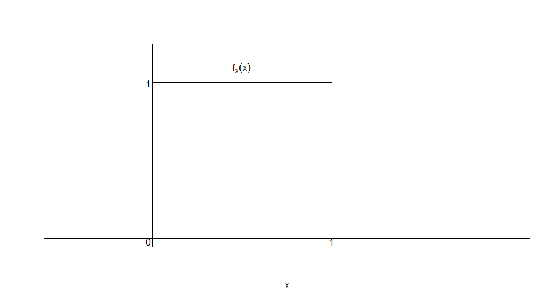
\includegraphics[width=0.95\textwidth,height=0.75\textheight]{uniform_pdf3.pdf}%
\end{figure}%
%EndExpansion


%TCIMACRO{\TeXButton{EndFrame}{\end{frame}}}%
%BeginExpansion
\end{frame}%
%EndExpansion

%TCIMACRO{\TeXButton{BeginFrame}{\begin{frame}}}%
%BeginExpansion
\begin{frame}%
%EndExpansion

\frametitle{Continuous uniform mean}

The expected value of $X$ is%
\begin{eqnarray*}
E\left[ X\right] &=&\int_{a}^{b}\frac{x}{\left( b-a\right) }dx \\
&=&\left. \frac{x^{2}}{2\left( b-a\right) }\right\vert _{a}^{b} \\
&=&\frac{b^{2}}{2\left( b-a\right) }-\frac{a^{2}}{2\left( b-a\right) } \\
&=&\frac{a+b}{2}
\end{eqnarray*}

\begin{example} 
When $a=0$ and $b=1$, then $E\left[ X\right] =\frac{1}{2}$.
\end{example} 
%TCIMACRO{\TeXButton{EndFrame}{\end{frame}}}%
%BeginExpansion
\end{frame}%
%EndExpansion

%TCIMACRO{\TeXButton{BeginFrame}{\begin{frame}}}%
%BeginExpansion
\begin{frame}%
%EndExpansion

\frametitle{Continuous uniform variance}

The variance of $X$ is%
\begin{eqnarray*}
Var\left( X\right) &=&\int_{a}^{b}\left( x-\left( \frac{a+b}{2}\right)
\right) ^{2}\frac{1}{b-a}dx \\
&=&E\left[ X^{2}\right] -E\left[ X\right] ^{2}
\end{eqnarray*}

We know the second term
\begin{equation*}
E\left[ X\right] ^{2}=\left( \frac{a+b}{2}\right) ^{2},
\end{equation*}

so we've just to work out%
\begin{eqnarray*}
E\left[ X^{2}\right] &=&\int_{a}^{b}\frac{x^{2}}{b-a}dx =\left. \frac{x^{3}}{3\left( b-a\right) }\right\vert _{a}^{b} \\
&=&\frac{b^{3}-a^{3}}{3\left( b-a\right) } = \frac{(b-a)\left( ab+a^{2}+b^{2}\right)}{3\left( b-a\right) } \\
&=&\frac{\left( ab+a^{2}+b^{2}\right) }{3}.
\end{eqnarray*}


%TCIMACRO{\TeXButton{EndFrame}{\end{frame}}}%
%BeginExpansion
\end{frame}%
%EndExpansion

%TCIMACRO{\TeXButton{BeginFrame}{\begin{frame}}}%
%BeginExpansion
\begin{frame}%
%EndExpansion

\frametitle{Continuous uniform variance}

Putting together, we get that the variance of $X$:%
\begin{eqnarray*}
Var\left( X\right) &=&\frac{\left( ab+a^{2}+b^{2}\right) }{3}-\left( \frac{%
a+b}{2}\right) ^{2} \\
&=&\frac{1}{12}\left( a-b\right) ^{2}
\end{eqnarray*}

\begin{example} [cont'd] 
When $a=0$ and $b=1$, then $Var\left( X\right) =\frac{1}{12}$.
\end{example} 
\end{frame}%
%EndExpansion


\begin{frame}%
%EndExpansion

\frametitle{Continuous uniform variance}

\begin{example} 
Let $X \sim U(0,10)$. Then its pdf is $f_X(x) = 1/10=0.1$ for $x\in[0,10]$ and zero otherwise. The pdf plot is:

\begin{figure}[ptb]\centering
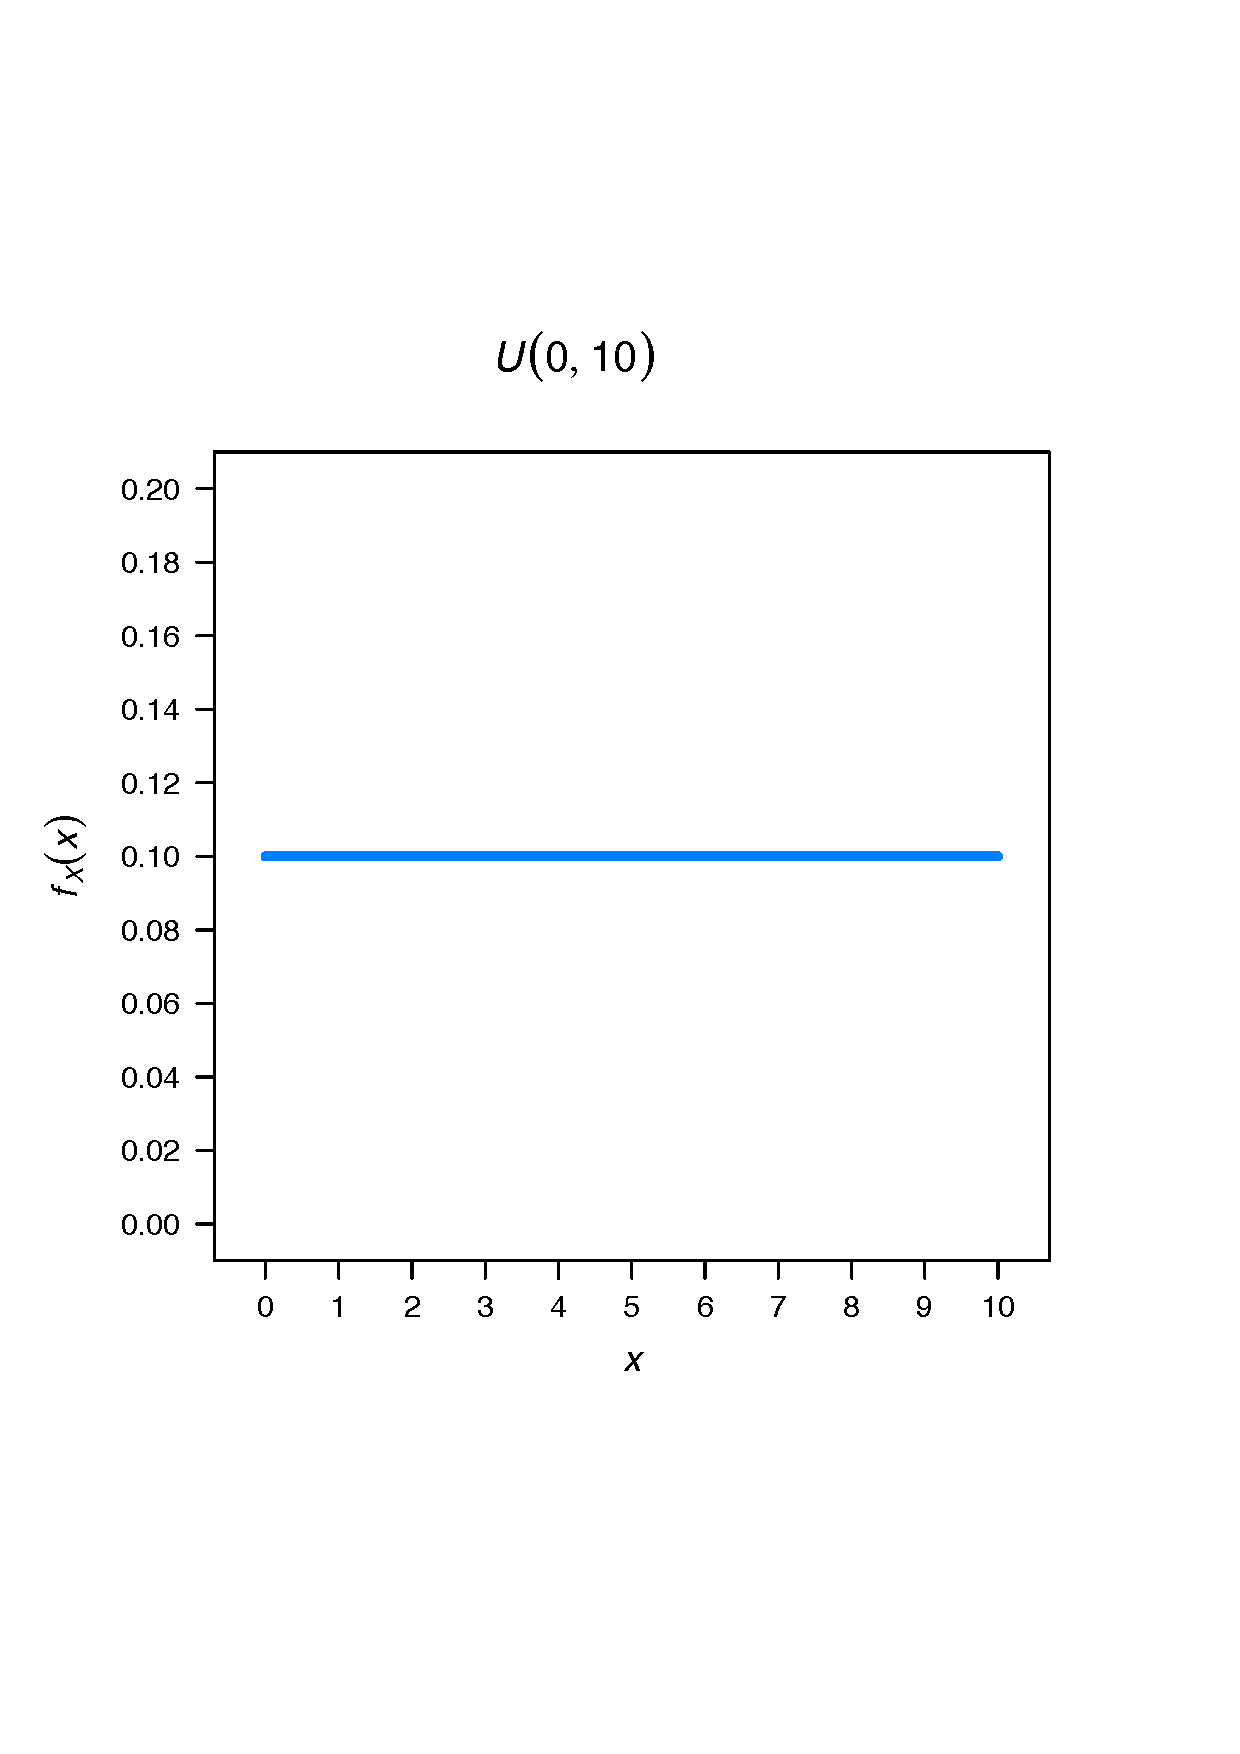
\includegraphics[width=0.45\textwidth,height=0.65\textheight]{Unif_Diego.pdf}%
\end{figure}%

\end{example} 
\end{frame}%


\begin{frame}%
%EndExpansion

\frametitle{Continuous uniform variance}

\begin{example}[cont'd]
 

\begin{figure}[ptb]\centering
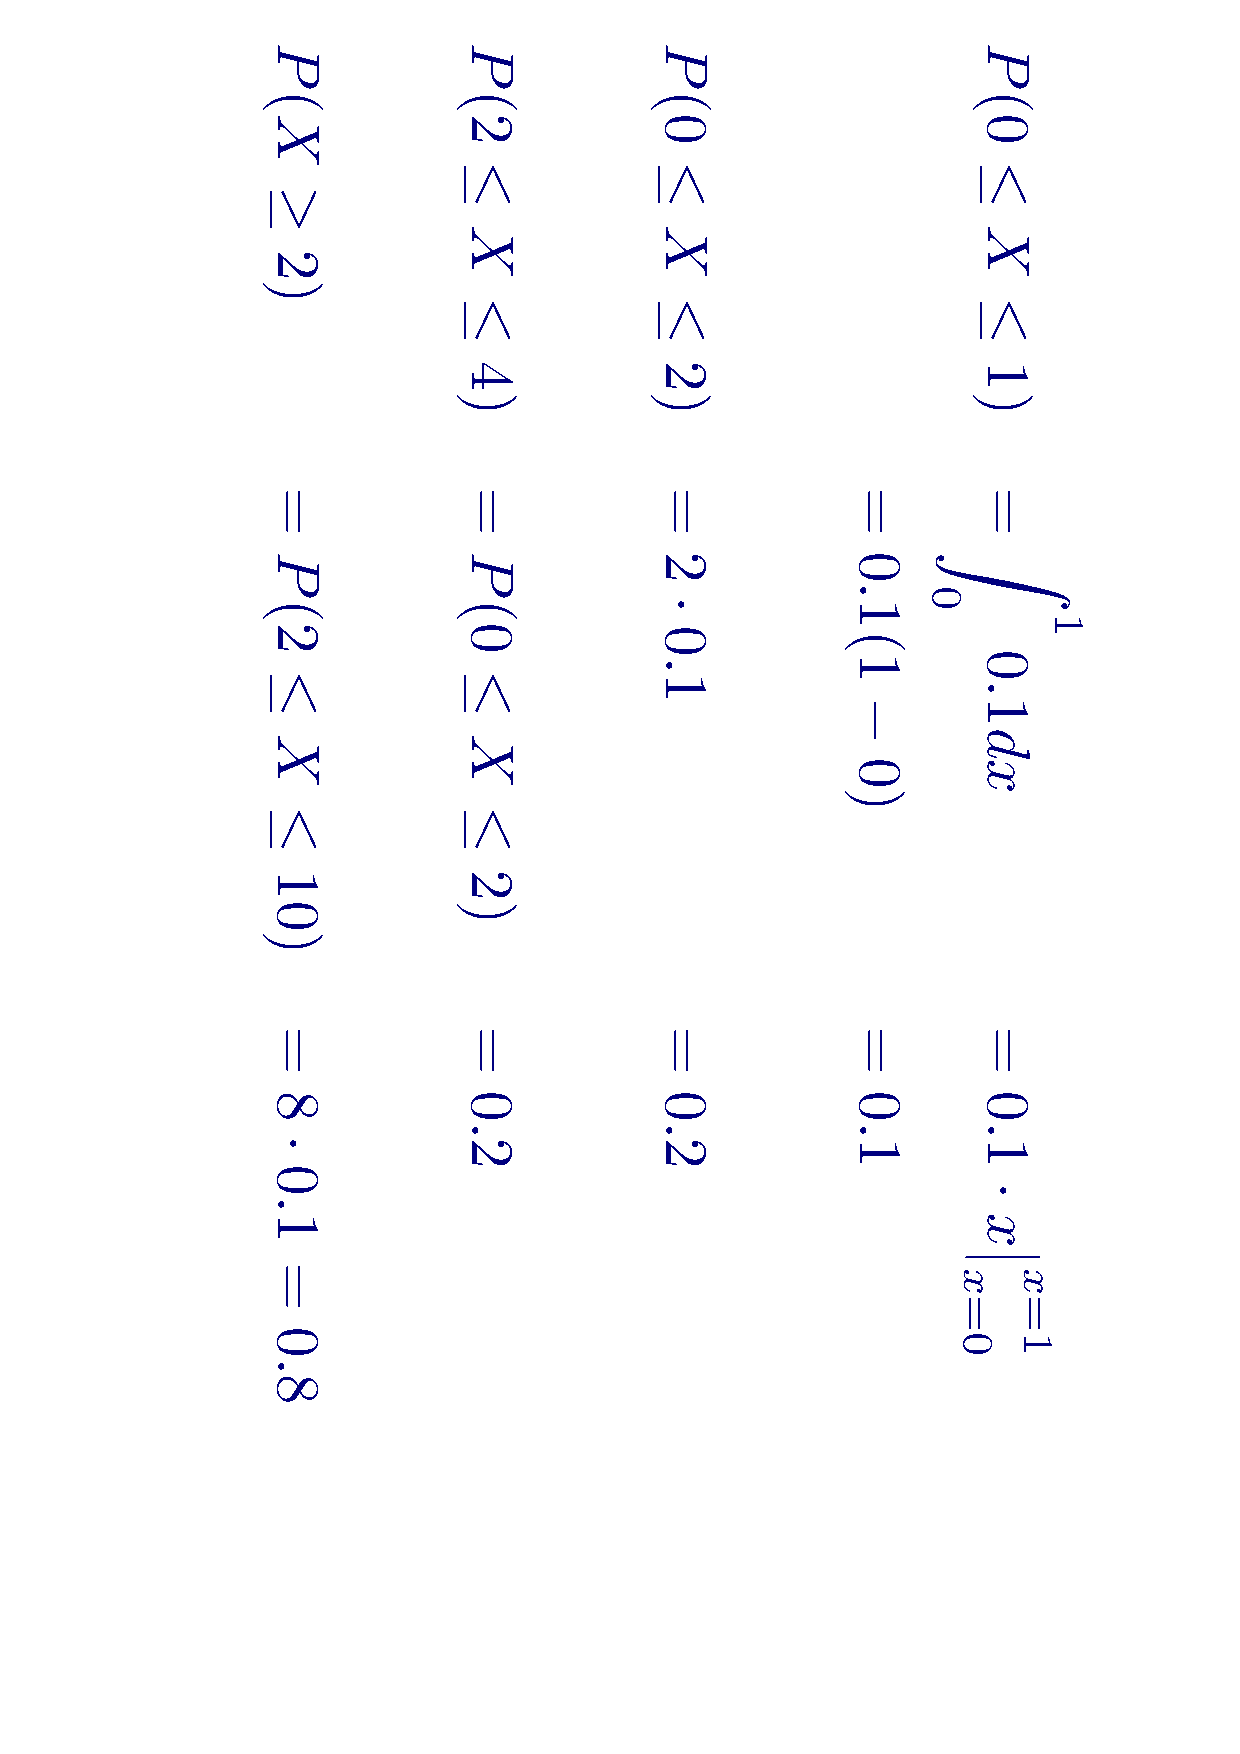
\includegraphics[width=0.5\textwidth,height=0.9\textheight, angle= 90]{Unif_Diego_Calc.pdf}%
\end{figure}%



\end{example} 
\end{frame}%

\begin{frame}%
\frametitle{Continuous uniform variance}

\begin{example}[cont'd]
 
...and for $P(X\geq 2)$, 
\begin{figure}[ptb]\centering
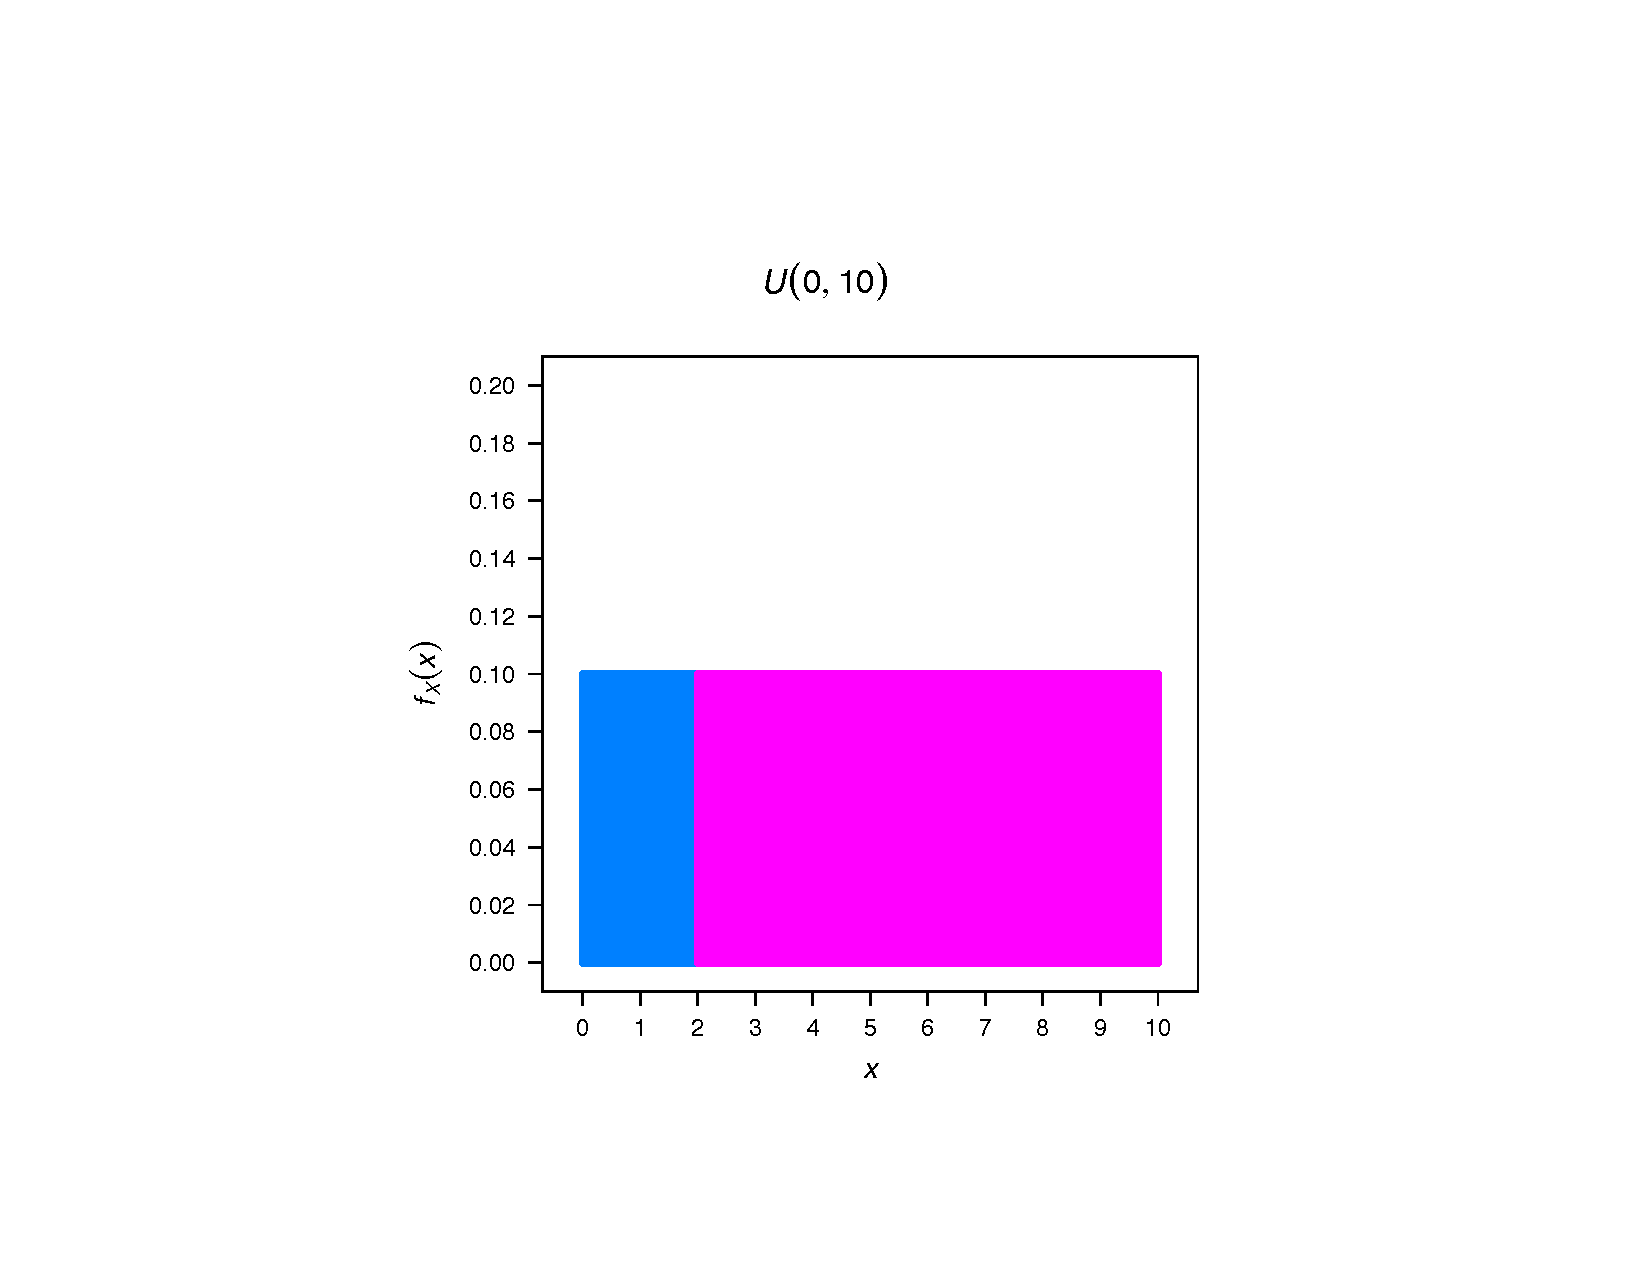
\includegraphics[width=0.45\textwidth,height=0.55\textheight, angle= 0]{CDF_Diego.pdf}%
\end{figure}%



\end{example} 
\end{frame}%




%TCIMACRO{\TeXButton{BeginFrame}{\begin{frame}}}%
%BeginExpansion
\begin{frame}%
%EndExpansion

\frametitle{Normal (Gaussian) distribution [A brief history]}

The Normal distribution was ``discovered" in the eighteenth
century when scientists observed an astonishing degree of
regularity in the behavior of measurement errors. They found that
the patterns (distributions) that they observed, and which they
attributed to chance, could be closely approximated by continuous
curves which they christened the ``normal curve of errors".
 
\vspace{0.4cm}
 
The mathematical properties of these curves were first studied by
\begin{stepitemize}
\item Abraham de Moivre (1667-1745),
\item Pierre Laplace (1749-1827), and then
\item Karl Gauss (1777-1855), who also lent his name to the
distribution.
\end{stepitemize}

%TCIMACRO{\TeXButton{EndFrame}{\end{frame}}}%
%BeginExpansion
\end{frame}%
%EndExpansion

%TCIMACRO{\TeXButton{BeginFrame}{\begin{frame}}}%
%BeginExpansion





\begin{frame}%
%EndExpansion

\frametitle{The Normal distribution}

\begin{definition}
A variable $X$ is said to have a \textbf{Gaussian} or \textbf{normal}
distribution, with mean $\mu $ and variance $\sigma ^{2}$, if its pdf is given by
\begin{equation*}
\phi_{(\mu,\sigma)}(x) =\frac{1}{\sqrt{2\pi \sigma ^{2}}}\exp^{ \left\{ -\frac{1%
}{2\sigma ^{2}}\left( x-\mu \right) ^{2}\right\}}~~-\infty<x<\infty\,.
\end{equation*}
For simplicity we denote this by writing $X\sim \N\left( \mu ,\sigma ^{2}\right) $. 
\end{definition}

\begin{remark}
\begin{stepitemize}
\item A normal distribution is completely characterised by its mean $\mu $ and its variance $\sigma ^{2}$. Infinitely many different normal distributions are obtained by varying the parameters $\mu $ and $\sigma ^{2}$.
\item A normal random variable $X$ can take any value $x\in\mathbb{R}$.
\end{stepitemize}
\end{remark}

%TCIMACRO{\TeXButton{EndFrame}{\end{frame}}}%
%BeginExpansion
\end{frame}%
%EndExpansion

%TCIMACRO{\TeXButton{BeginFrame}{\begin{frame}}}%
\begin{frame}%

\frametitle{Normal distributions}

The pdf of the normal distribution is
\begin{stepitemize}
\item `bell-shaped'
\item symmetric
\item unimodal
\item the mean, median and mode are all equal.
\end{stepitemize}
\begin{figure}[ptb]\centering
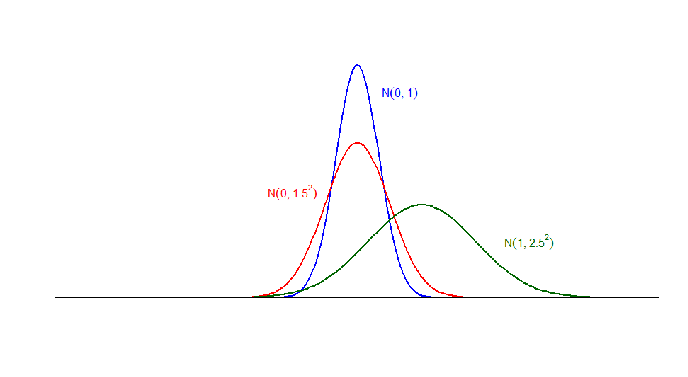
\includegraphics[width=0.95\textwidth,height=0.75\textheight]{normals4.pdf}%
\end{figure}%
\end{frame}%


\begin{frame}%

\frametitle{Normal distributions}

\begin{figure}[ptb]\centering
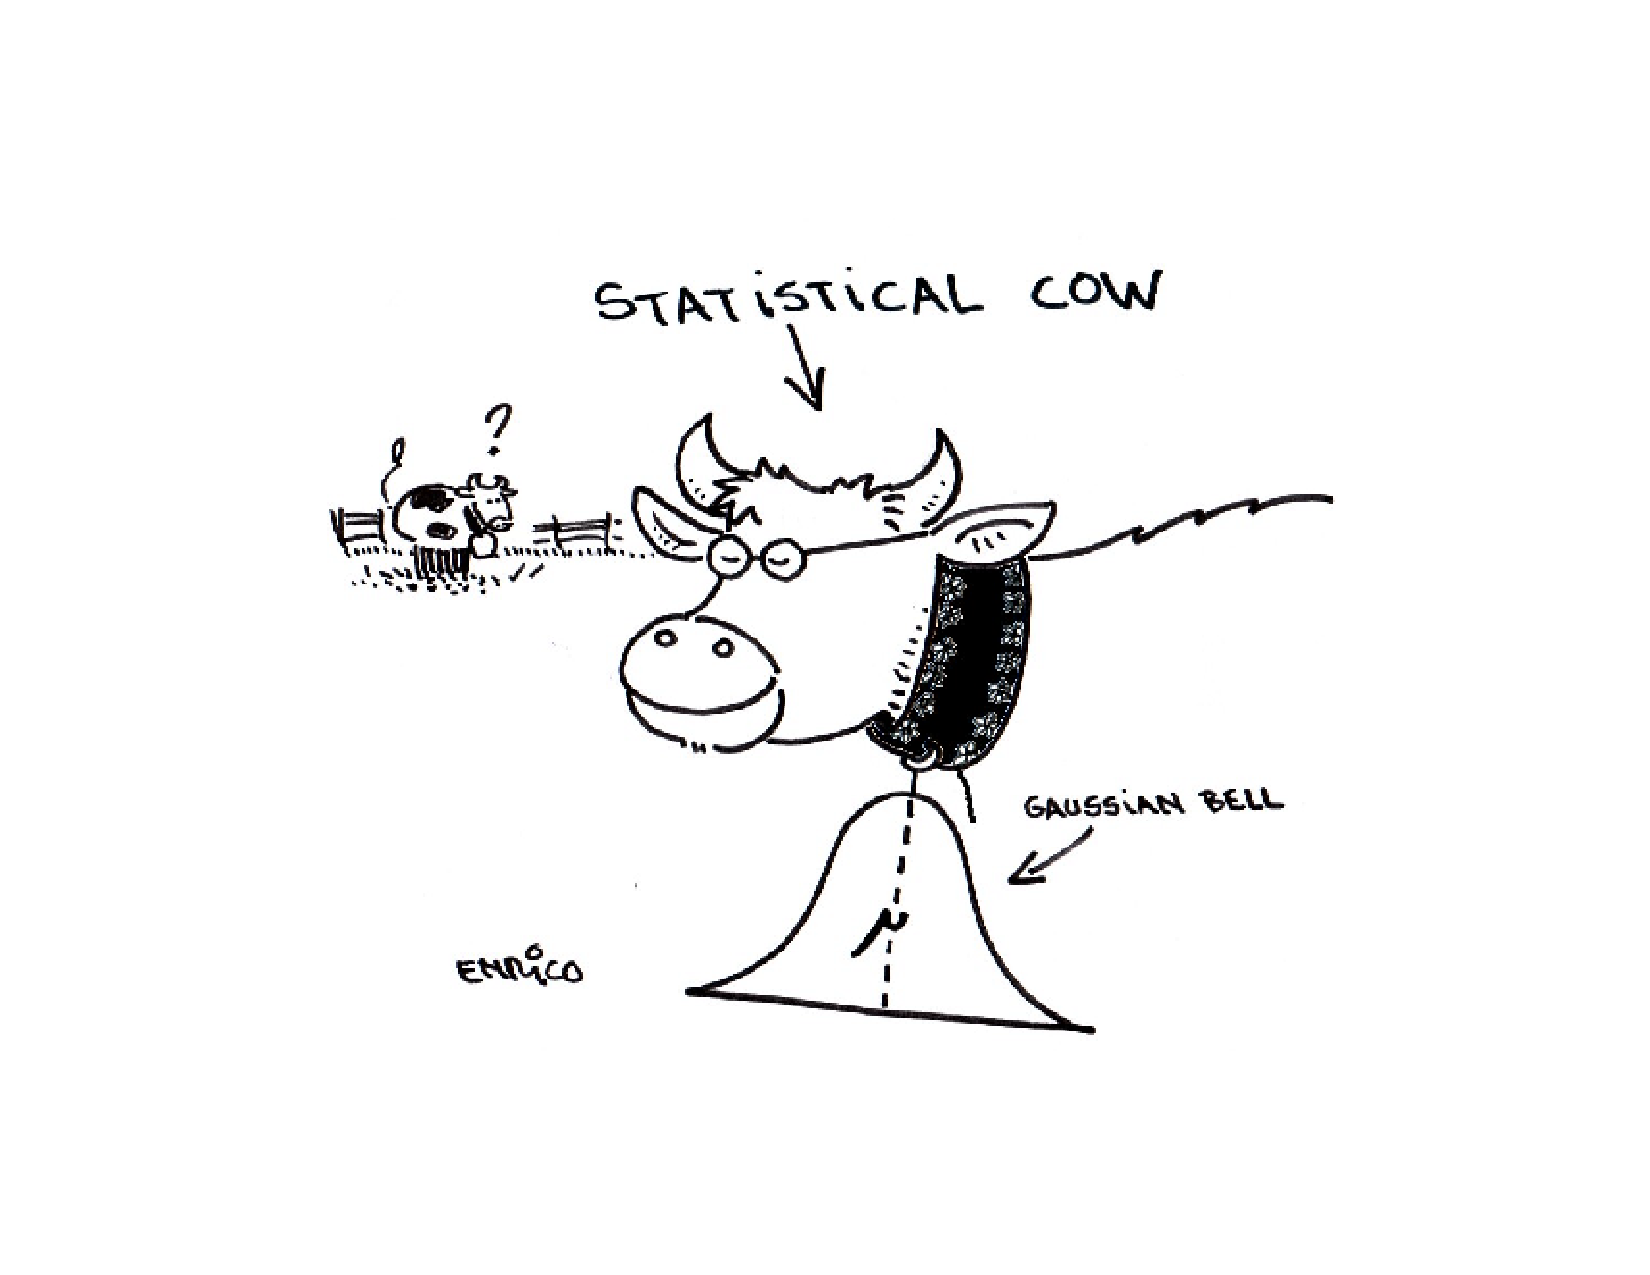
\includegraphics[width=0.95\textwidth,height=0.75\textheight]{Cow.pdf}%
\end{figure}%

\end{frame}%

\begin{frame}%

\frametitle{Normal distributions}

First let us establish that $\phi_{(\mu,\sigma)}(x)$ can serve as a
genuine density function. Integrating with respect to $x$ using
\textit{integration by substitution} we obtain
\begin{eqnarray*}
\int_{-\infty}^{\infty}\phi_{(\mu,\sigma)}(x)dx&=&
\int_{-\infty}^{\infty}\frac{1}{\sqrt{2\pi\sigma^2}}\exp^{\{-\frac{(x-\mu)^2}{2\sigma^2}\}}dx
\\
 &=&\int_{-\infty}^{\infty}\frac{1}{\sqrt{2\pi}}\exp^{\{-\frac{z^2}{2}\}}dz
\end{eqnarray*}
where $z=(x-\mu)/\sigma$. But the second integral on the right
hand side equals
$$
\frac{2}{\sqrt{2\pi}}\underbrace{\int_0^{\infty}\exp^{\{-z^2/2\}}dz}_{={\sqrt{2\pi}} \big/ {2}}
$$
which is \textbf{a known standard integral}.
%  \item When $X\sim \N\left( \mu ,\sigma ^{2}\right) $ the same property is verified in a similar way using integration by substitution, the standard integral and basic properties of the integral.
%\end{stepenumerate}
%
%TCIMACRO{\TeXButton{EndFrame}{\end{frame}}}%
%BeginExpansion
\end{frame}%
%EndExpansion

%TCIMACRO{\TeXButton{BeginFrame}{\begin{frame}}}%
%BeginExpansion
\begin{frame}%
%EndExpansion

\frametitle{The standard Normal distribution}

Thus:
\begin{itemize}
  \item The function $\phi_{(\mu,\sigma)}(x)$ does indeed define the pdf of a random variable with a mean of $\mu$ and a variance of $\sigma^2$.
\item This was established by transforming from $X$ to $Z$ via the substitution $Z=(X-\mu)/\sigma$. Such a variable
is said to be standardised. Note also that the resulting integrand
$$
\frac{1}{\sqrt{2\pi}}\exp^{\{-\frac{z^2}{2}\}}=\phi_{(0,1)}(z)\,,
$$
is the pdf of a random variable $Z\sim \N(0,1)$.
\item If $Z\sim \N(0,1)$ then $Z$ is called a \color{blue}Êstandard normal random variate \color{black} because
$
\textsf{E}[Z]=0$ and $\textsf{Var}(Z)=1$

\item Because of the special role that the standard normal distribution has in
calculations involving the normal distribution its pdf is given the special notation 
$$\phi(z)=\phi_{(0,1)}(z).$$
\end{itemize}

%TCIMACRO{\TeXButton{BeginFrame}{\begin{frame}}}%
%BeginExpansion
\end{frame}%
%EndExpansion


%TCIMACRO{\TeXButton{BeginFrame}{\begin{frame}}}%
%BeginExpansion
\begin{frame}%
%EndExpansion

\frametitle{The standard Normal distribution}

The basic feature that underlies calculations involving the Normal distribution:
\begin{stepitemize}
\item $$X\sim \N\left( \mu ,\sigma ^{2}\right)\Leftrightarrow Z=\frac{\left( X-\mu \right) }{\sigma }\sim \N\left( 0,1\right)$$
\begin{stepitemize}
\item We can always transform from $X$ to $Z$  by  `shifting' and `re-scaling':%
\begin{equation*}
Z=\frac{X-\mu }{\sigma } \ (\text{for the random variable}) \quad\mbox{and}\quad z=\frac{x-\mu }{\sigma }\,  \ (\text{for its values}) ,
\end{equation*}
\item and return back to $X$ by a `re-scaling' and `shifting':%
\begin{equation*}
X=\sigma Z+\mu  \ (\text{for the random variable}) \quad\mbox{and}\quad x=\sigma z+\mu\, \ (\text{for its values}) .
\end{equation*}
\end{stepitemize}
\item Thus statements about a Normal random variable can always be translated into equivalent statements about a standard Normal random variable, and vice versa.
\end{stepitemize}

%TCIMACRO{\TeXButton{EndFrame}{\end{frame}}}%
%BeginExpansion
\end{frame}%
%EndExpansion


\begin{frame}%
%EndExpansion

\frametitle{The Normal CDF}
In pictures:
Start from $X \sim \mathcal{N}(5,3)$; then define $Y=X-5$, which is a recentered/shifted $X$ (it's centered at 0 and has the same variance as $X$); finally define $Z$, which is a recentered/shifted and rescaled $X$ (it's centered at 0 and has unit variance). 

\begin{figure}[ptb]\centering
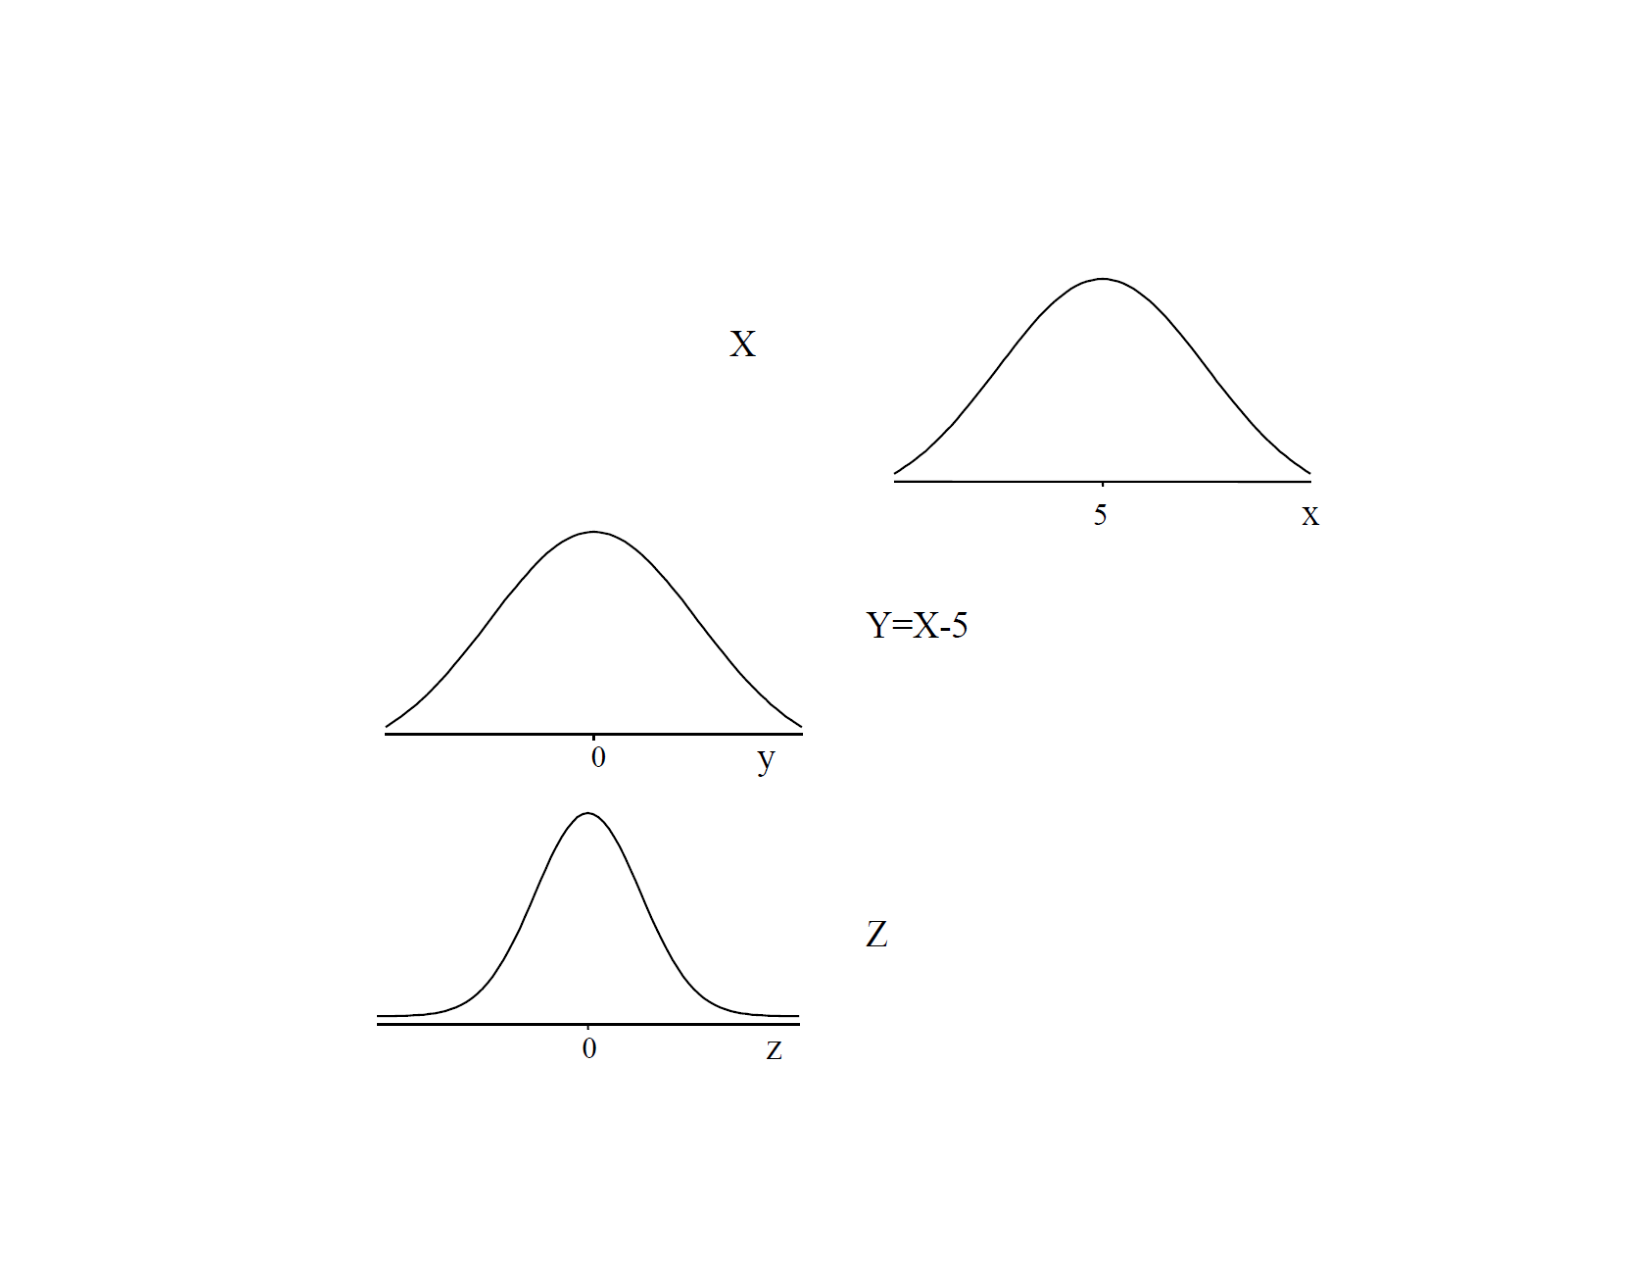
\includegraphics[width=0.8\textwidth,height=0.65\textheight]{Std_Diego.pdf}%
\end{figure}%



\end{frame}

%TCIMACRO{\TeXButton{BeginFrame}{\begin{frame}}}%
%BeginExpansion
\begin{frame}%
%EndExpansion

\frametitle{The Normal CDF}
In formulae:
\begin{stepitemize}
\item For $X\sim \N\left( \mu ,\sigma ^{2}\right) $, the CDF is given by%
$$
\Phi_{(\mu,\sigma)}\left( x\right) =\int_{-\infty }^{x}\frac{1}{\sqrt{2\pi \sigma ^{2}}}\exp^{ \left\{ -\frac{1}{2\sigma ^{2}}\left( t-\mu \right) ^{2}\right\}} dt
$$
\item To calculate $\Phi_{(\mu,\sigma)}\left( x\right)=\Pr(\{X\leq x\})$ we use integration by substitution, once again, to give
\begin{eqnarray*}
\Pr(\{ X\leq x\} )&=&\int_{-\infty}^x\frac{1}{\sqrt{2\pi\sigma^2}}\exp^{\left\{-\frac{(t-\mu)^2}{2\sigma^2}\right\}}dt\\
 &=&\int_{-\infty}^z\phi(s)ds\\
  &=&P(\{Z\leq z\})
\end{eqnarray*}
where $z=(x-\mu)/\sigma$, $s=(t-\mu)/\sigma$ and $ds=dt/\sigma$.
\item The required probability has been mapped into a corresponding probability for a standard Normal random variable.
\end{stepitemize}

%TCIMACRO{\TeXButton{EndFrame}{\end{frame}}}%
%BeginExpansion
\end{frame}%
%EndExpansion

%TCIMACRO{\TeXButton{BeginFrame}{\begin{frame}}}%
%BeginExpansion
\begin{frame}%
%EndExpansion

\frametitle{The Normal CDF}

\begin{stepitemize}
\item We can evaluate the probabilities
$$
\Pr(\{Z\leq z\})=\Phi(z)=\int_{-\infty}^z\phi(s)ds
$$
either directly using a computer or indirectly via Standard Normal
Tables.
\item Standard Normal Tables give values of the integral $\Phi(z)$ for various values of $z\geq 0$. (The tables are themselves
calculated using a computer, of course.)
\item For negative values of $z$ the symmetry property of $\phi(z)$ (\textit{i.e.} $\phi(z)=\phi(-z)$) tells us that
$$
\Phi(-z)=1-\Phi(z)\,.
$$
\item Similarly, if $X\sim \N\left( \mu ,\sigma ^{2}\right) $ then
\begin{eqnarray*}
\Pr(\{x_1<X\leq x_2\})&=&\Pr(\{z_1<Z\leq z_2\})\\
 &=&\Phi(z_2)-\Phi(z_1)
 \end{eqnarray*}
where $z_1=(x_1-\mu)/\sigma$ and $z_2=(x_2-\mu)/\sigma$.

\end{stepitemize}

%TCIMACRO{\TeXButton{EndFrame}{\end{frame}}}%
%BeginExpansion
\end{frame}%
%EndExpansion

%TCIMACRO{\TeXButton{BeginFrame}{\begin{frame}}}%
%BeginExpansion
\begin{frame}%
%EndExpansion

\frametitle{Standard Normal Tables}

\begin{stepitemize}
\item Standard Normal Tables give values of the standard normal integral $\Phi(z)$ for various values of $z\geq 0$.  Values for negative $z$ are obtained via symmetry.
%\item Other Normal tables give either $1-\Phi(z)$ (tail area) or $\Phi(z)-0.5$!
\end{stepitemize}


\begin{figure}[ptb]\centering
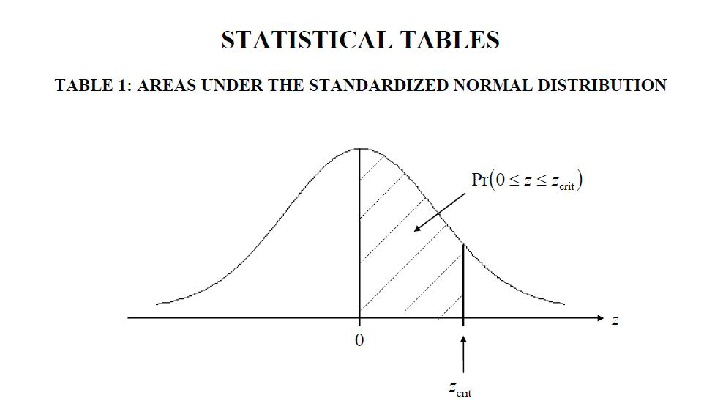
\includegraphics[width=0.95\textwidth,height=0.75\textheight]{bell_curve__5.pdf}%
\end{figure}%
\end{frame}%


\begin{frame}%
\begin{figure}[ptb]\centering
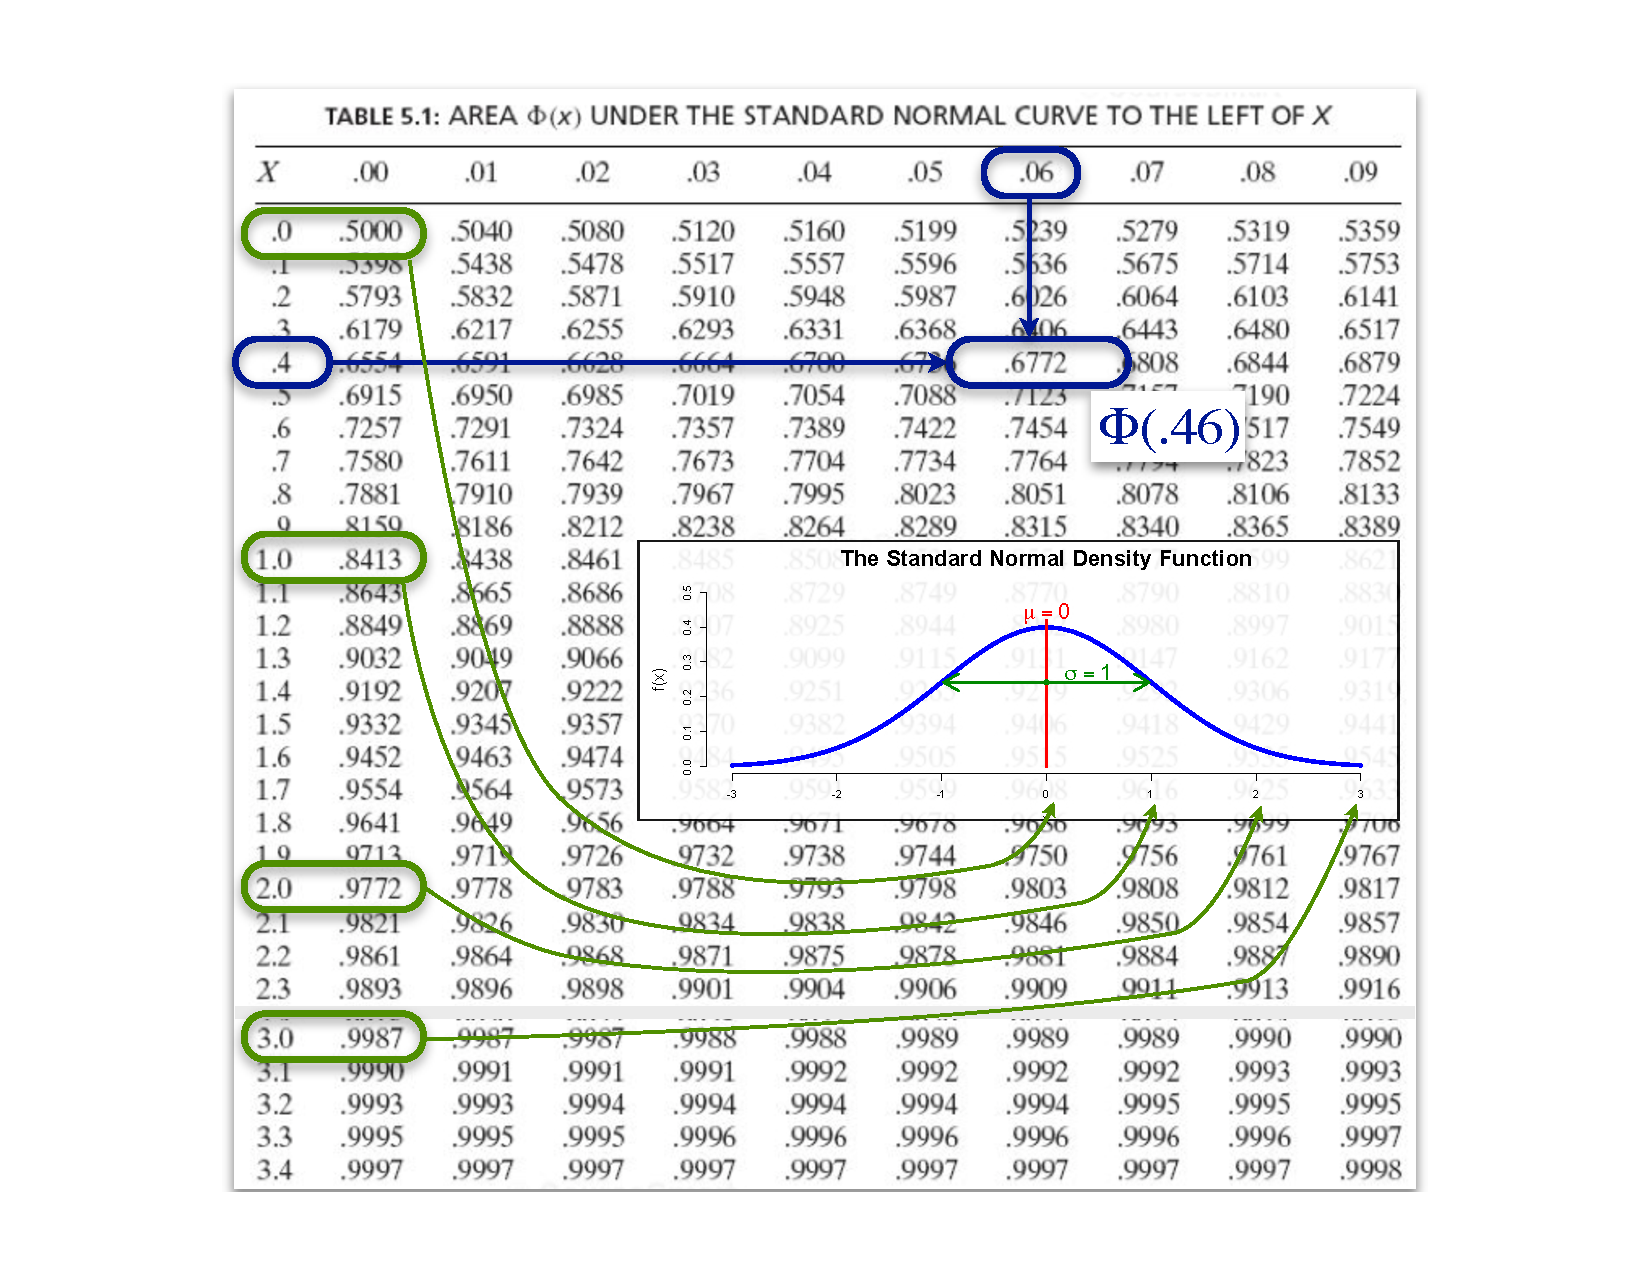
\includegraphics[width=0.9\textwidth,height=0.95\textheight]{myTableGauss.pdf}%
\end{figure}%
\end{frame}%

\begin{frame}%
\frametitle{Standard Normal Tables}
.... and you can use these tables to compute integrals/probabilities of the type: 
\begin{figure}[ptb]\centering
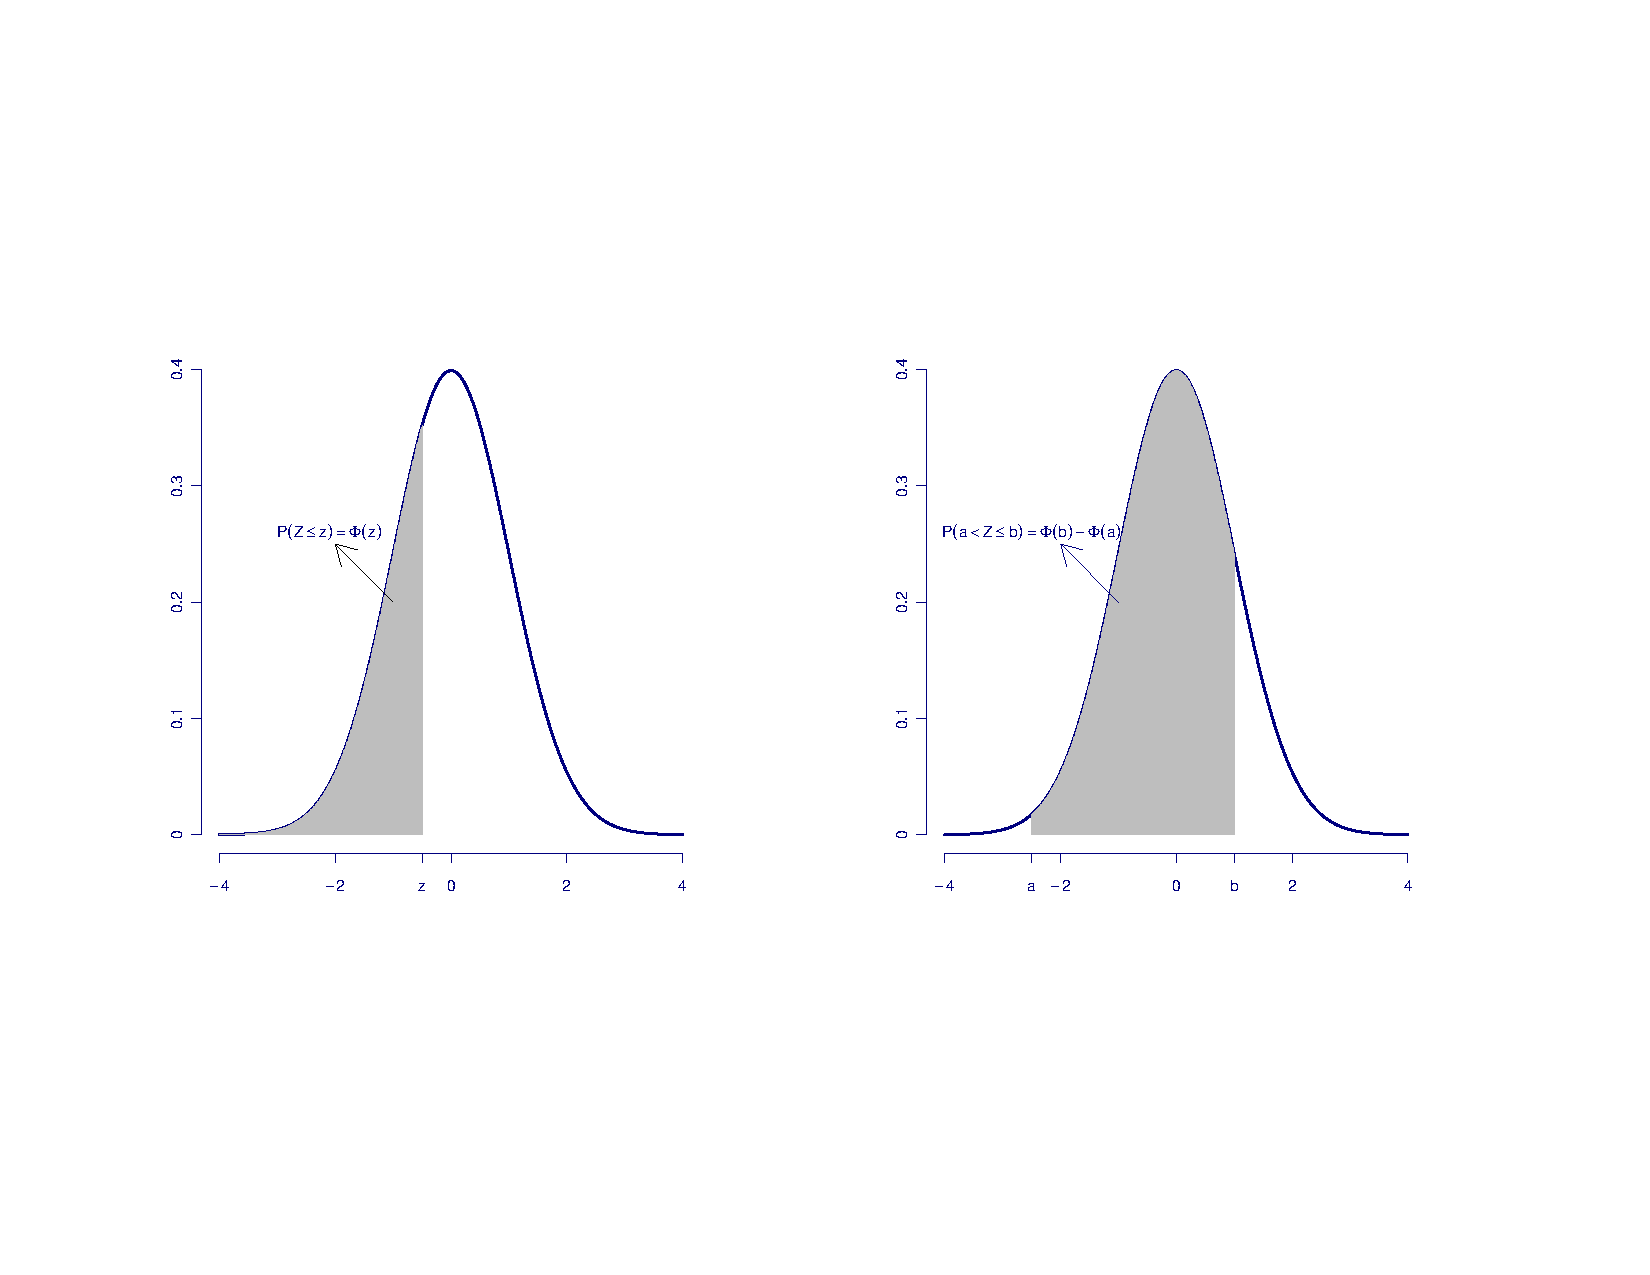
\includegraphics[height=2in, width=4in]{CDF_pr.pdf}%
\end{figure}%
\end{frame}%

\begin{frame}%
\frametitle{Standard Normal Tables}

\begin{example}[Prob of $Z$]


\noindent
\begin{tabular}{ll}
$P(\{Z\leq 1\})$ & $\approx0.8413\bigskip $ \\
$P(\{Z\leq 1.96\})$ & $\approx0.9750\bigskip $ \\
$P(\{Z\geq 1.96\})$ & $=1-P(\{Z\leq 1.96\})$ $\approx1-0.9750=0.0250\bigskip $\\
$P(\{Z\geq -1\})$ & $=P(\{Z\leq 1\})\approx0.8413\bigskip $ \\ 
$P(\{Z\leq -1.5\})$ & $=P(\{Z\geq 1.5\}) =1-P(\{Z\leq 1.5\})$ $\approx1-0.9332=0.0668$%
\end{tabular}

\end{example}
\end{frame}%

\begin{frame}%
\frametitle{Standard Normal Tables}

\begin{example}[cont'd]

\begin{tabular}{ll}
& $P(\{0.64\leq Z\leq 1.96\})=$ \\ 
& $P(\{Z\leq 1.96\})-P(\{Z\leq 0.64\})$ \\ 
& $\approx 0.9750-0.7389=0.2361\bigskip $ \\ 
& $P(\{-0.64\leq Z\leq 1.96\})$ \\ 
& $=P(\{Z\leq 1.96\})-P(\{Z\leq -0.64\})$ \\
& $=P(\{Z\leq 1.96\})-(1-P(\{Z\leq 0.64\}))$ \\ 
& $\approx0.9750-(1-0.7389)=0.7139\bigskip $ \\ 
& $P(\{-1.96\leq Z\leq -0.64\})$ \\ 
& $=P(\{0.64\leq Z\leq 1.96\})$ \\ 
& $\approx0.2361$%
\end{tabular}
\end{example}
\end{frame}%

\begin{frame}%
%EndExpansion

\frametitle{Some properties of the Normal distribution}


\begin{figure}[ptb]\centering
\ \hspace{0.6cm} One $\sigma$ \hspace{2.4cm} Two $\sigma$s \hspace{2.5cm} Three $\sigma$s \hspace{3cm}
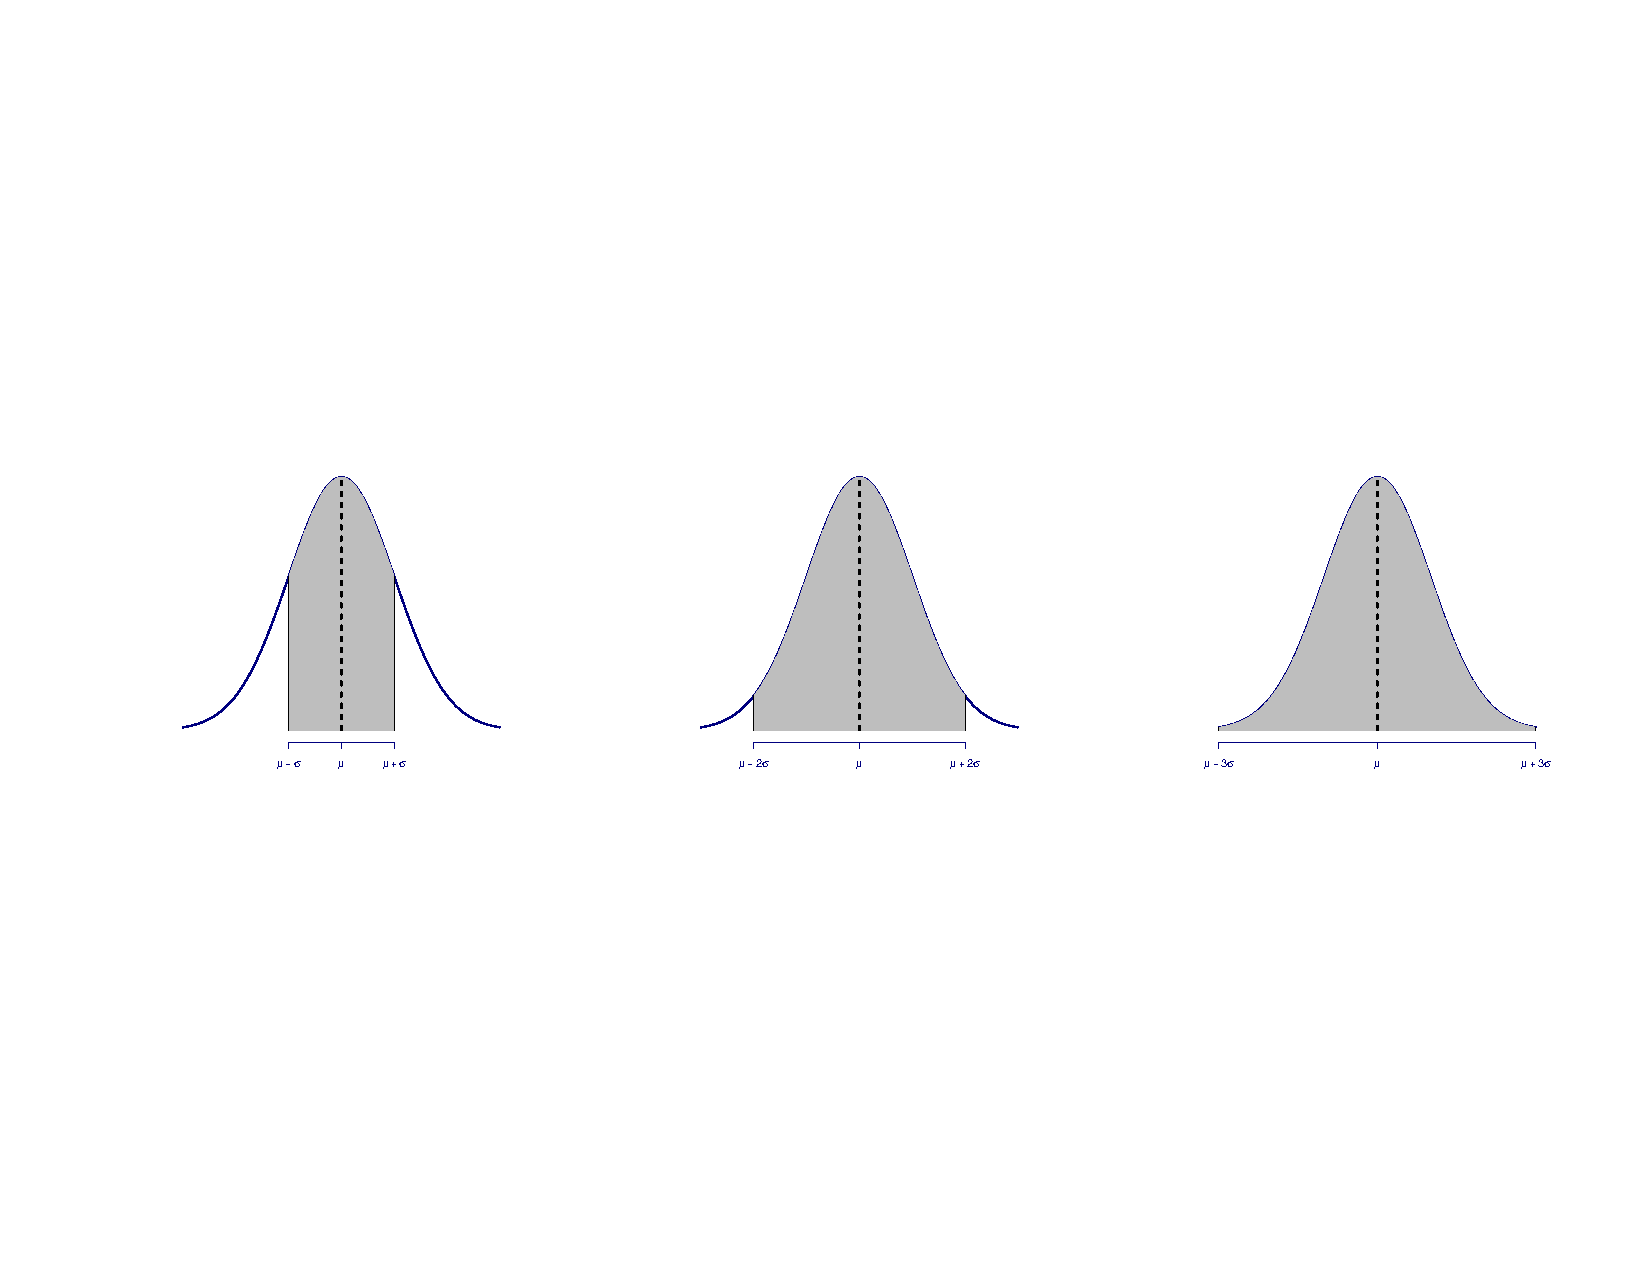
\includegraphics[height=1.5in, width=4.5in]{Areas_Normal.pdf}%
\end{figure}%
The shaded areas under the pdfs are (approximately) equivalent to $0.683$, $0.954$ and $0.997$, 
respectively. So we state  the following ....

\end{frame}%



\begin{frame}%
%EndExpansion

\frametitle{Some properties of the Normal distribution}




\textbf{... rule `68 -- 95 -- 99.7'}: \\ \vspace{0.5cm}


If $X$ is a Normal random variable, $X \sim \N(\mu, \sigma^2)$, its realization has approximately a probability of \\ \vspace{0.5cm}

\begin{tabular}{llll}
$\bullet$
&
$68 \, \%$ 
&
\mbox{of being in the interval}
&
$\lbrack \mu - \sigma, \, \mu + \sigma \rbrack$;\\[0.2cm]
$\bullet$
&
$95 \, \%$  
&
\mbox{of being in the interval}
&
$\lbrack \mu - 2 \, \sigma, \, \mu + 2 \, \sigma \rbrack$;\\[0.2cm]
$\bullet$
&
$99.7 \, \%$  
&
\mbox{of being in the interval}&
$\lbrack \mu - 3 \, \sigma, \, \mu + 3 \, \sigma \rbrack$.\\[0.2cm]
\end{tabular}
\end{frame}


\begin{frame}%
%EndExpansion

\frametitle{Some properties of the Normal distribution}

\begin{stepitemize}
\item For $X\sim \N\left( \mu ,\sigma ^{2}\right) $ 
\begin{equation*}
E\left[ X\right] =\mu \text{ and }Var\left( X\right) =\sigma ^{2}.
\end{equation*}

\item If $a$ is a number, then 
\begin{eqnarray*}
X+a &\sim &\N\left( \mu +a,\sigma ^{2}\right) \\
aX &\sim &\N\left( a\mu ,a^{2}\sigma ^{2}\right).
\end{eqnarray*}

\item If $X\sim \N\left( \mu ,\sigma ^{2}\right) $ and $Y\sim \N\left( \alpha
,\delta ^{2}\right) $, and $X$ and $Y$ are \textbf{independent} then%
\begin{equation*}
X+Y\sim \N\left( \mu +\alpha ,\sigma ^{2}+\delta ^{2}\right).
\end{equation*}

\end{stepitemize}

%TCIMACRO{\TeXButton{EndFrame}{\end{frame}}}%
%BeginExpansion
\end{frame}%
%EndExpansion

%TCIMACRO{\TeXButton{BeginFrame}{\begin{frame}}}%
%BeginExpansion
\begin{frame}%
%EndExpansion

\frametitle{The sum of two independent Normals}


\begin{figure}[ptb]\centering
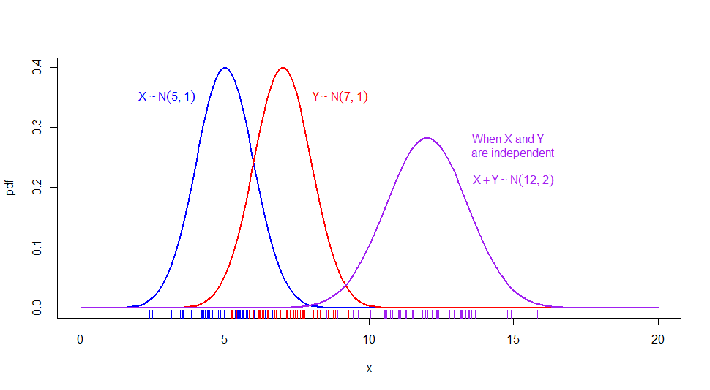
\includegraphics[width=0.95\textwidth,height=0.7\textheight]{sum_of_two_independent_normals_with_rug__1.pdf}%
\end{figure}


Locations of $n=30$ sampled values of $X,$ $Y$, and $X+Y$ shown as tick marks under each respective density.

\end{frame}%


\begin{frame}%
%EndExpansion

\frametitle{Normal: an example}

\begin{example}

On the highway A2 (in the Luzern area), the speed is limited to $80$ $km/h$. A radar measures the speeds of all the cars. 
Assuming that the registered speeds are distributed according to a Normal law with mean $72$ $km/h$ and standard error $8$ $km/h$: \vspace{0.2cm}
\begin{enumerate}
  \item what is the proportion of the drivers who will have to pay a penalty for high speed? \vspace{0.2cm}
  \item knowing that in addition to the penalty, a speed higher than $30$ $km/h$ (over the max allowed speed) implies a withdrawal of the driving license, what is the proportion of the drivers who  will lose their driving license among those who will have a to pay a fine?
\end{enumerate}
  
\end{example}
\end{frame}



\begin{frame}%
%EndExpansion

\frametitle{Normal: an example}

\begin{example}[cont'd]
Let $X$ be the random variable expressing the registered speed: $X \sim \mathcal{N}(72,64)$.
\begin{enumerate}
  \item Since a driver has to pay if its speed is above  $80$ $km/h$, the proportion of drivers paying a penalty is expressed  through $P(X>80)$:
\begin{equation*}
P(X>80)= P\left(Z>\frac{80-72}{8} \right)=1-\Phi(1) \simeq 16 \%
\end{equation*}
where $Z \sim \mathcal{N}(0,1)$.
  \item We are looking for the conditional probability of a recorded speed greater than 110 \underline{given that} the driver has had already to pay a fine:
  \begin{eqnarray*}
  P(X>110 \vert X>80) &=&  \frac{P(\{X>110\} \bigcap \{X>80\})}{P(X>80)} \\
   &=& \frac{P(X>110)}{P(X>80)} = \frac{1- \Phi((110-72)/8)}{1-\Phi(1)}\approx \frac{0}{16\%}\simeq 0.
  \end{eqnarray*}


\end{enumerate}



\end{example}
\end{frame}


%\begin{frame}%
%EndExpansion

%\frametitle{... it's all about normality...}
%
%
%\begin{figure}[ptb]\centering
%\includegraphics[natheight=7.389in, natwidth=13.4859in, height=2.4031in, width=4.7426in]{RU_Normal.pdf}%
%\end{figure}
%
%
%\end{frame}%
%


\begin{frame}%

\frametitle{The Chi-squared distribution}

\begin{definition}
If $Z_{1},Z_{2},\ldots ,Z_{n}$ are independent standard Normal random
variables, then%
\begin{equation*}
X=Z_{1}^{2}+Z_{2}^{2}+\cdots +Z_{n}^{2}
\end{equation*}%
has a chi-squared distribution with $n$ degrees of freedom. Write as $X\sim \chi ^{2}(n)$.
\end{definition}

$X\sim \chi ^{2}(n)$ can take only \textbf{positive }values. Moreover, expected value and variance, for $X\sim \chi ^{2}(n)$, are:
\begin{eqnarray*}
E\left[ X\right] &=&n \\
Var\left( X\right) &=&2n
\end{eqnarray*}

If $X\sim \chi ^{2}(n)$ and $Y\sim \chi ^{2}(m)$ are \textbf{%
independent} then $X+Y\sim \chi ^{2}(n+m)$.


\end{frame}

\begin{frame}%

\frametitle{Some plots for the Chi-squared}

\begin{figure}[ptb]\centering
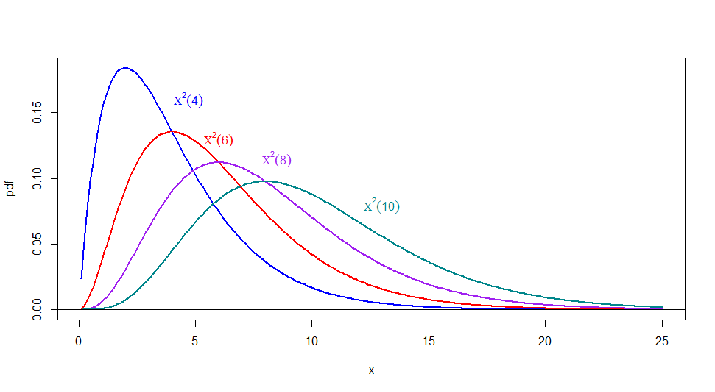
\includegraphics[height=2.6143in, width=4.6643in]{chisquared_pdfs__2.pdf}%
\end{figure}

Probabilities for Chi-squared distributions may be obtained from a table

\end{frame}%

\begin{frame}%

\frametitle{Chi-squared table}


\begin{figure}[ptb]\centering
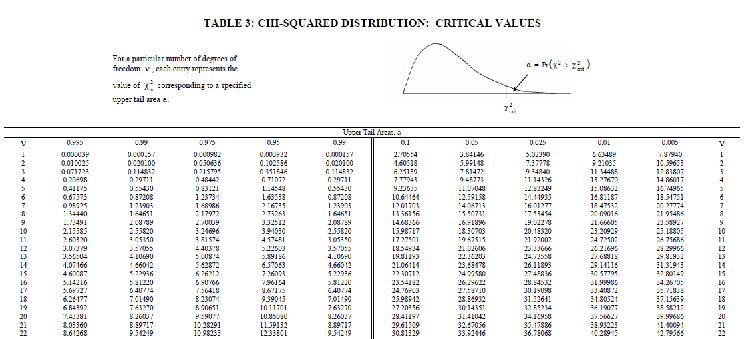
\includegraphics[height=2.2649in, width=4.9658in]{chisq_table__3.pdf}%
\end{figure}

\end{frame}%

\begin{frame}%

\frametitle{Chi-squared table (illustration of its use)}

\begin{example}

Let $X$ be a chi-squared random variable with 10 degrees-of-freedom. What is the value of its \underline{upper fifth percentile}? \vspace{0.6cm}

By definition, the upper fifth percentile is the chi-squared value $x$ (lower case!!!) such that the probability to the right of $x$ is $0.05$ (so the upper tail area is $5\%$).  To find such an $x$ we use the chi-squared table: \vspace{0.1cm}
\begin{itemize} 
\item setting $\mathcal{V} = 10$ in the first column on the left and getting the corresponding row \vspace{0.1cm}
\item finding the column headed by $P(X \geq x) = 0.05$. \vspace{0.1cm}
\end{itemize} 

Now, all we need to do is read the corresponding cell. What do we get? Well, the table tells us that the upper fifth percentile of a chi-squared random variable with 10 degrees of freedom is \textbf{18.30703}. 



\end{example}



\end{frame}%

\begin{frame}%

\frametitle{The Student-t distribution}

\begin{definition}
If $Z\sim \N(0,1)$ and $Y\sim \chi ^{2}(v)$ are \textbf{independent}
then%
\begin{equation*}
T=\frac{Z}{\sqrt{Y/v}}
\end{equation*}%
has a \textbf{Student-t} distribution with $v$ degrees of freedom. Write as $T\sim t_{v}$.
\end{definition}
\vspace{0.5cm}
$T\sim t_{v}\,$\ can take any value in $\mathbb{R}$. Expected value and variance for $T\sim t_{v}$ are 
\begin{eqnarray*}
E\left[ T\right] &=&0\text{, for }v>1 \\
Var\left( T\right) &=&\frac{v}{v-2}\text{, for }v>2.
\end{eqnarray*}

%TCIMACRO{\TeXButton{EndFrame}{\end{frame}}}%
%BeginExpansion
\end{frame}%
%EndExpansion

%TCIMACRO{\TeXButton{BeginFrame}{\begin{frame}}}%
%BeginExpansion
\begin{frame}%
%EndExpansion

\frametitle{Some Student-t distributions}
\begin{remark}
The pdf of $T\sim t_{v}$ is similar to a Normal (with mean zero) but with fatter tails. When $v$ is large (typically, $v \geq 120$) $t_{v}$ approaches $\N(0,1)$.
\end{remark}

\begin{figure}[ptb]\centering
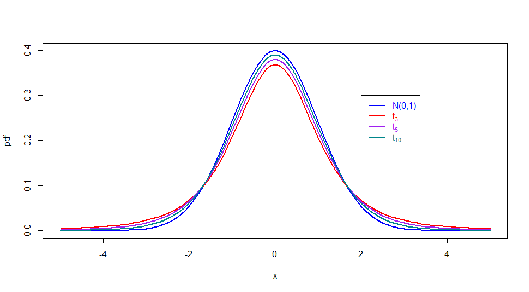
\includegraphics[height=1.9398in, width=3.5345in]{student_t__4.pdf}%
\end{figure}%
%EndExpansion


\end{frame}
\begin{frame}


\frametitle{Student-t table}

\begin{figure}[ptb]\centering
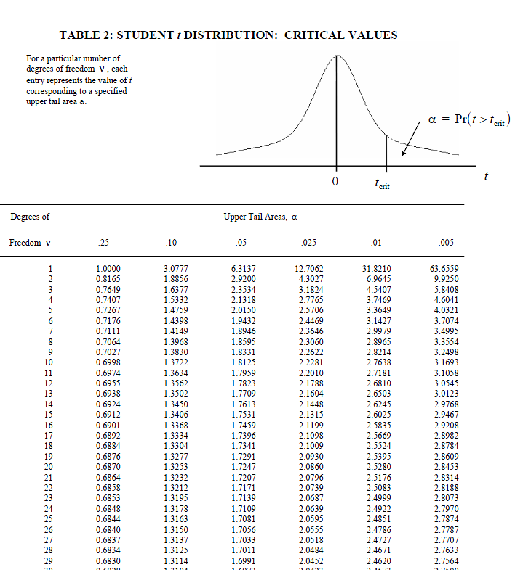
\includegraphics[height=3.8in, width=3.506in]{Student_t_table__5.pdf}%
\end{figure}

\end{frame}

\begin{frame}%

\frametitle{The F distribution}

\begin{definition}
If $X\sim \chi ^{2}(v_{1})$ and $Y\sim \chi ^{2}(v_{2})$ are \textbf{%
independent}, then%
\begin{equation*}
F=\frac{\frac{X}{v_{1}}}{\frac{Y}{v_{2}}},
\end{equation*}%
has an \textbf{F} distribution with $v_{1}$ `numerator' and $v_{2}$
`denominator' degrees of freedom. Write as $F\sim F_{v_{1},v_{2}}$.
\end{definition}

$F\sim F_{v_{1},v_{2}}\,$\ can take only \textbf{positive }values. Expected value and variance for $F\sim F_{v_{1},v_{2}}$ (note that the order of the degrees of freedom is important!).
\begin{eqnarray*}
E\left[ F\right] &=&\frac{v_{2}}{v_{2}-2}\text{, for }v_{2}>2 \\
Var\left( F\right) &=&\frac{2v_{2}^{2}\left( v_{1}+v_{2}-2\right) }{%
v_{1}\left( v_{2}-2\right) ^{2}\left( v_{2}-4\right) }\text{, for }v_{2}>4.
\end{eqnarray*}

\end{frame}

\begin{frame}
\frametitle{Some F distributions}

\begin{figure}[ptb]\centering
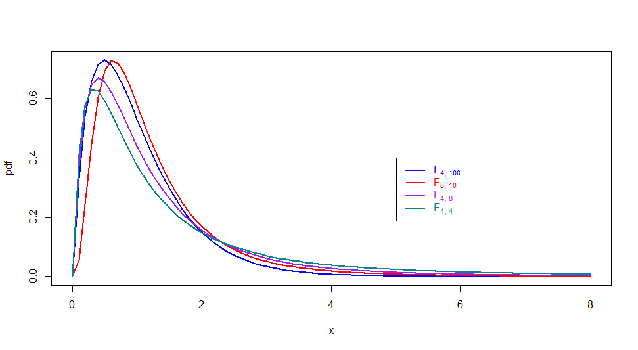
\includegraphics[height=2.3324in, width=4.2462in]{F-dist_pds__6.pdf}%
\end{figure}%
\end{frame}%

\begin{frame}
\frametitle{F distribution table (5\% upper tail)}


\begin{figure}[ptb]\centering
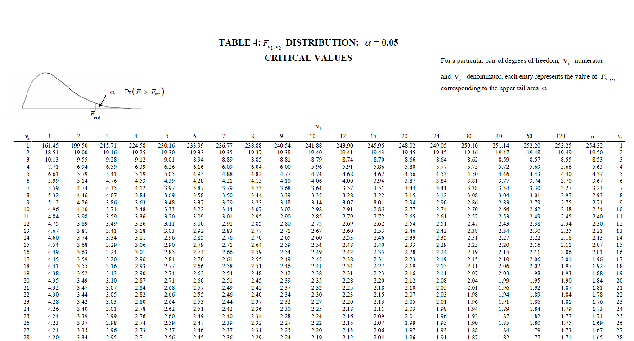
\includegraphics[height=2.2753in, width=4.2263in]{Fdist_table__7.pdf}%
\end{figure}%
%EndExpansion

%TCIMACRO{\TeXButton{EndFrame}{\end{frame}}}%
%BeginExpansion
\end{frame}%
%EndExpansion




%TCIMACRO{\TeXButton{BeginFrame}{\begin{frame}}}%
%BeginExpansion
\begin{frame}%
%EndExpansion

\frametitle{The lognormal distribution}

\begin{definition}
 $Y$ has a \textbf{lognormal distribution} when 
 $$\ln \left( Y\right) =X$$
has a Normal distribution. We write $Y\sim $ \emph{lognormal}$\left( \mu ,\sigma ^{2}\right) $. 
\end{definition}

\vspace{0.4cm}

If $Y\sim $ \emph{lognormal}$\left( \mu ,\sigma ^{2}\right) $ then%
\begin{eqnarray*}
E\left[ Y\right] &=&\exp^{ \left( \mu +\frac{1}{2}\sigma ^{2}\right)} \\
Var(Y) &=&\exp^{ \left( 2\mu +\sigma ^{2}\right)} \left( \exp^{ \left( \sigma
^{2}\right)} -1\right).
\end{eqnarray*}


%TCIMACRO{\TeXButton{EndFrame}{\end{frame}}}%
%BeginExpansion
\end{frame}%


\begin{frame}%
%EndExpansion

\frametitle{The lognormal distribution}


Let us just see some plots... more to come later...
\begin{figure}[ptb]\centering
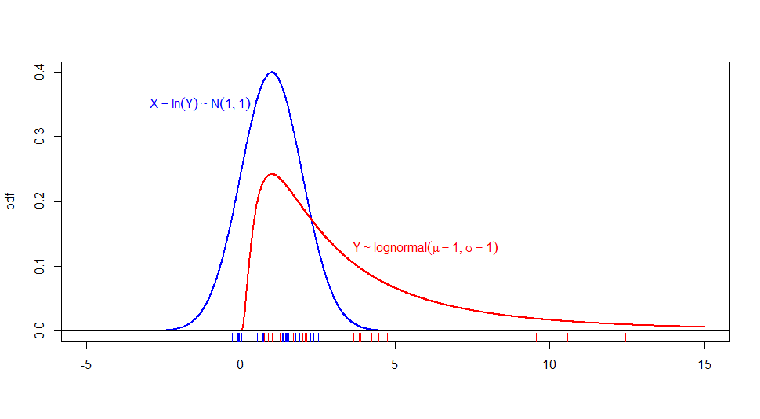
\includegraphics[height=2.4856in, width=4.5in]{lognormal_with_rug__8.pdf}%
\end{figure}%
%EndExpansion

\end{frame}%


\begin{frame}
\frametitle{Exponential distribution}


\begin{definition}
Let $X$ be a  continuous random variable, having the following  characteristics:
\begin{itemize}
\item[--]       $X$ is defined on the positive real numbers $\left( 0;\infty \right) $ --- namely $\mathbb{R}^+$;  
\item[--]       the pdf and CDF are 
\bea
f_X(x)=\lambda \exp^{ -\lambda x},\lambda
>0; &
F_X(x)=1-\exp (-\lambda x); \nn \eea 
\end{itemize}
then we say that $X$ has an exponential distribution. We write $X\sim$ \text{Exp$(\lambda)$}.
\end{definition}

For $X\sim$ \text{Exp$(\lambda)$} we have that:  
\begin{small}
\bea
E[X]=\int_{0}^{\infty }xf_X(x )dx= 1/\lambda & \text{and} &   Var(X)=\int_{0}^{\infty }x^{2}f_X(x )dx-E^{2}(X)=1/\lambda ^{2}. \nn
\eea
\end{small}

\begin{remark}
$X$ is typically applied to model the waiting time until an event occurs, when events are always occurring at a random rate $\lambda >0$. Moreover, the sum of independent exponential random variables has a Gamma distribution (see tutorial).
\end{remark}
\end{frame}%


\begin{frame}
\frametitle{Exponential distribution}
\begin{small}
\begin{example}
Let $X\sim$ \text{Exp}$(\lambda)$, with $\lambda =0.5$. Thus 
$$f_X(x) = \left\{ \begin{array}{ll}
0.5 \exp (-0.5x) & x>0\\
0 & \text{otherwise}
\end{array} \right.$$
Then, find the CDF.
%
\vspace{0.1cm}

For $x>0$, we have
\begin{eqnarray*}
F_{X}(x) & = & \int_{0}^{x}f_{X}(u)du\\
& = & 0.5\Big( -2\exp (-0.5u)\Big) \bigl|_{u=0}^{u=x}\\
& = & 0.5(-2\exp (-0.5x)+2\exp (0))\\
& = & 1-\exp (-0.5x)
\end{eqnarray*}

so, finally, 

$$F_X(x) = \left\{ \begin{array}{ll}
0 & x \leq 0 \\
1-\exp (-0.5x)& x>0
\end{array} \right.$$
\end{example}
\end{small}
\end{frame}%



\begin{frame}
\frametitle{Exponential distribution}


\begin{example} [cont'd]

...and a graphical illustration, with varying $\lambda$

\begin{figure}[ptb]\centering
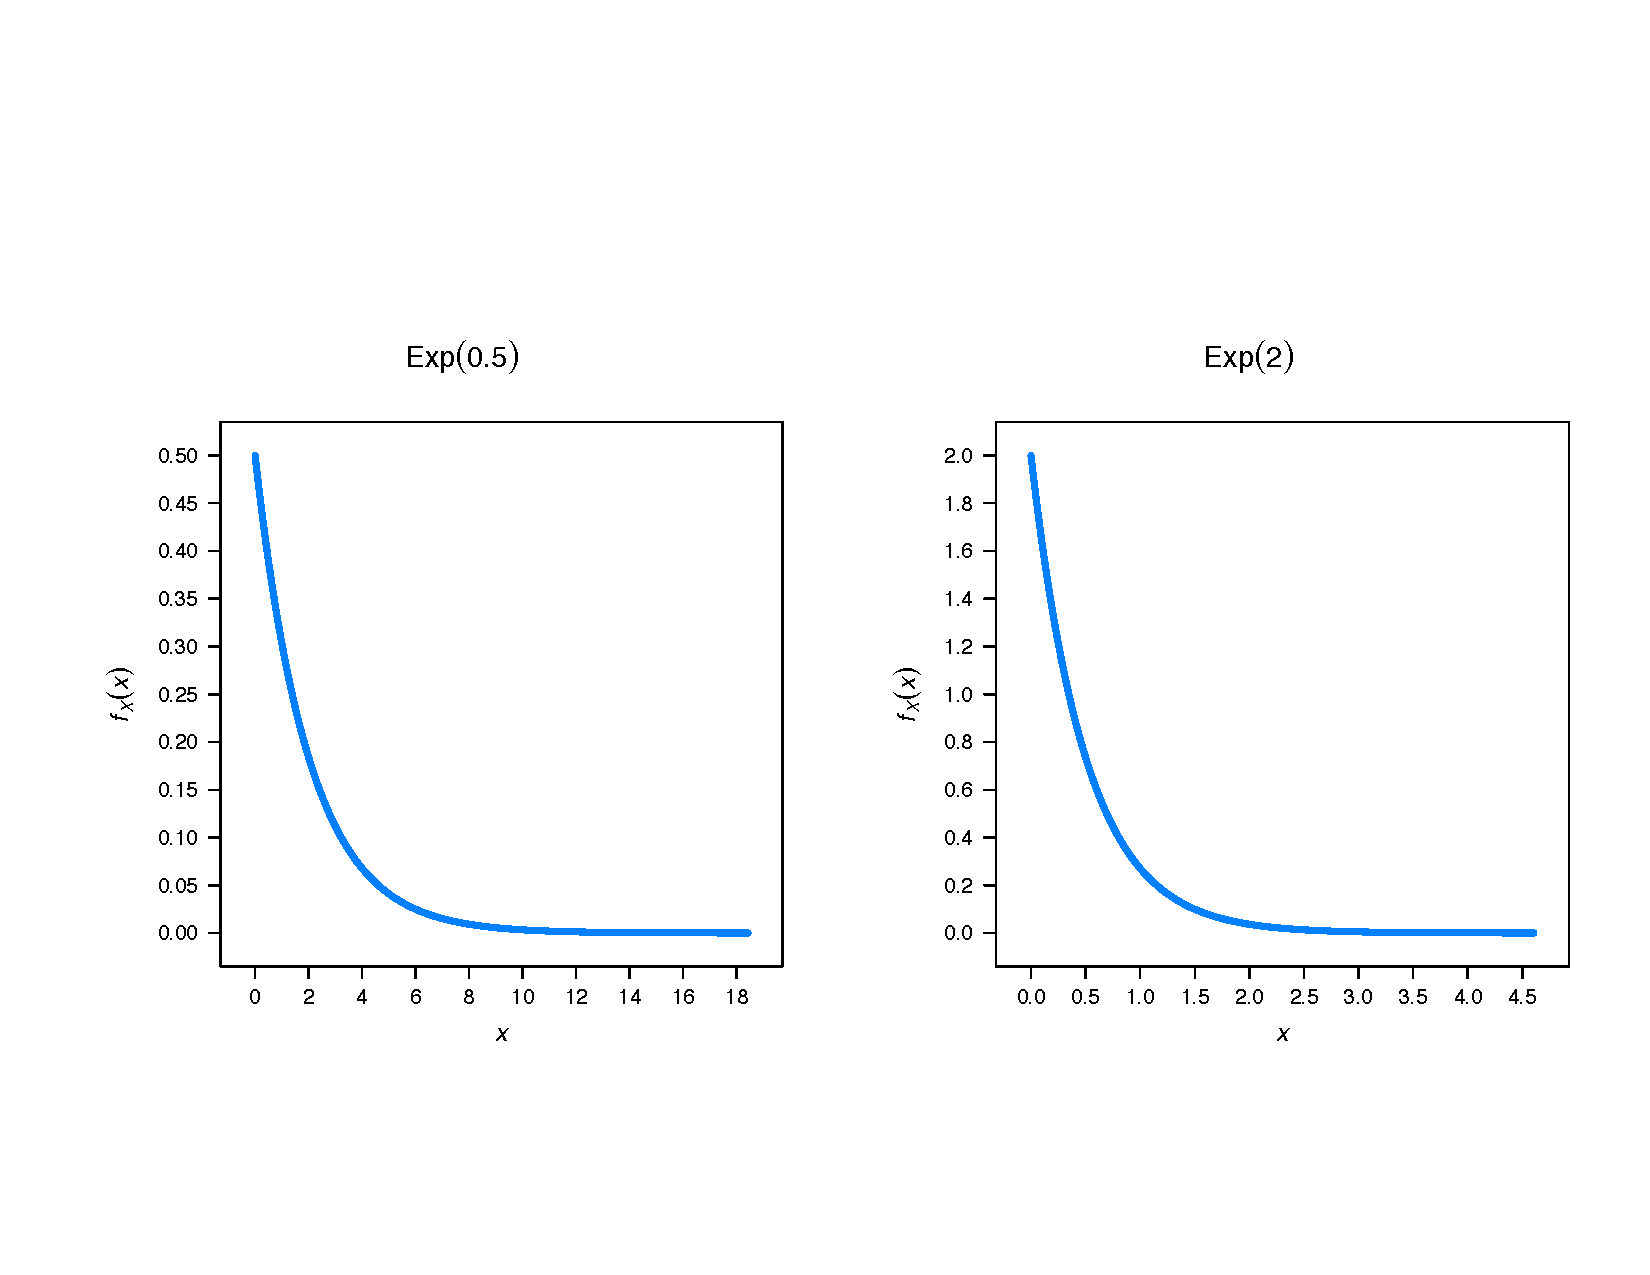
\includegraphics[height=2.4856in, width=4.5in]{Exp_Diego.pdf}%
\end{figure}%

\end{example}
\end{frame}%




\begin{frame}

\frametitle{Transformation of variables}

\begin{stepitemize}
\item Consider a random variable $X$

\item Suppose we are interested in $Y=\psi(X)$, where $\psi $ is a \textbf{%
one to one function}

\begin{stepitemize}
\item A \textbf{function }$\psi \left( x\right) $\textbf{\ is one to one}
(1-to-1) if there are no two numbers, $x_{1},x_{2}$ in the domain of $\psi $
such that $\psi \left( x_{1}\right) =\psi \left( x_{2}\right) $ but $%
x_{1}\neq x_{2}$.

\item A sufficient condition for $\psi \left( x\right) $ to be 1-to-1 is
that it be monotonically increasing (or decreasing) in $x$.

\item Note that the \textbf{inverse} of a 1-to-1 function $y=\psi \left(
x\right) $ is a 1-to-1 function $\psi^{-1}\left( y\right) $ such that 
\begin{equation*}
\psi ^{-1}\left( \psi \left( x\right) \right) =x\text{ and }\psi \left( \psi
^{-1}\left( y\right) \right) =y.
\end{equation*}
\end{stepitemize}

\item To transform $X$ to $Y$, we need to consider all the values $x$ that $%
X $ can take

\item We first transform $x$ into values $y=\psi (x)$
\end{stepitemize}

%TCIMACRO{\TeXButton{EndFrame}{\end{frame}}}%
%BeginExpansion
\end{frame}%
%EndExpansion

%TCIMACRO{\TeXButton{BeginFrame}{\begin{frame}}}%
%BeginExpansion
\begin{frame}%
%EndExpansion

\frametitle{Transformation of discrete random variables}

\begin{stepitemize}
\item To transform a discrete random variable $X$, into the random variable $%
Y=\psi (X)$, we transfer the probabilities for\textbf{\ each} $x$ to the values $%
y=\psi \left( x\right) $: 
\begin{equation*}
\begin{tabular}{l|cll|c}
\multicolumn{2}{l}{\emph{Probability function for }$X$} &  & 
\multicolumn{2}{l}{\emph{Probability function for }$X$} \\ 
&  &  &  &  \\ 
$X$ & $\Pr \left(\{ X=x_{i} \}\right) =p_{i}$ &  & $Y$ & $\Pr \left(\{
X=x_{i}  \}\right) =p_{i}$ \\ \cline{1-2}\cline{4-5}
$x_{1}$ & $p_{1}$ & $\qquad \Rightarrow \qquad $ & $\psi (x_{1})$ & $p_{1}$
\\ 
$x_{2}$ & $p_{2}$ &  & $\psi (x_{2})$ & $p_{2}$ \\ 
$x_{3}$ & $p_{3}$ &  & $\psi (x_{3})$ & $p_{3}$ \\ 
$\vdots $ & $\vdots $ &  & $\vdots $ & $\vdots $ \\ 
$x_{n}$ & $p_{n}$ &  & $\psi (x_{n})$ & $p_{n}$%
\end{tabular}%
\end{equation*}

\item Note that this is equivalent to applying the function $\psi \left(
\cdot \right) $ inside the probability statements:%
\begin{eqnarray*}
\Pr \left( \{ X=x_{i}  \}\right) &=&\Pr \left(  \{\psi \left( X\right) =\psi \left(
x_{i}\right)  \} \right) \\
&=&\Pr \left( \{ Y=y_{i} \} \right) \\
&=&p_{i}
\end{eqnarray*}
\end{stepitemize}

%TCIMACRO{\TeXButton{EndFrame}{\end{frame}}}%
%BeginExpansion
\end{frame}%
%EndExpansion

\begin{frame}%
\frametitle{Transformation of discrete random variables}
\begin{example} [option pricing]

Let us imagine that we are tossing a balanced coin ($p=1/2$), and when we get a ``Head'' ($H$) the stock price moves up of a factor $u$, but when we get a ``Tail'' ($T$) the price moves down of a factor $d$. We denote the price at time $t_1$  by $S_1(H)=u S_0 $ if the toss results in head ($H$), and by $S_1(T)=d S_0 $  if it results in tail ($T$). After the second toss, the price will be one of:
\begin{figure}[ptb]\centering
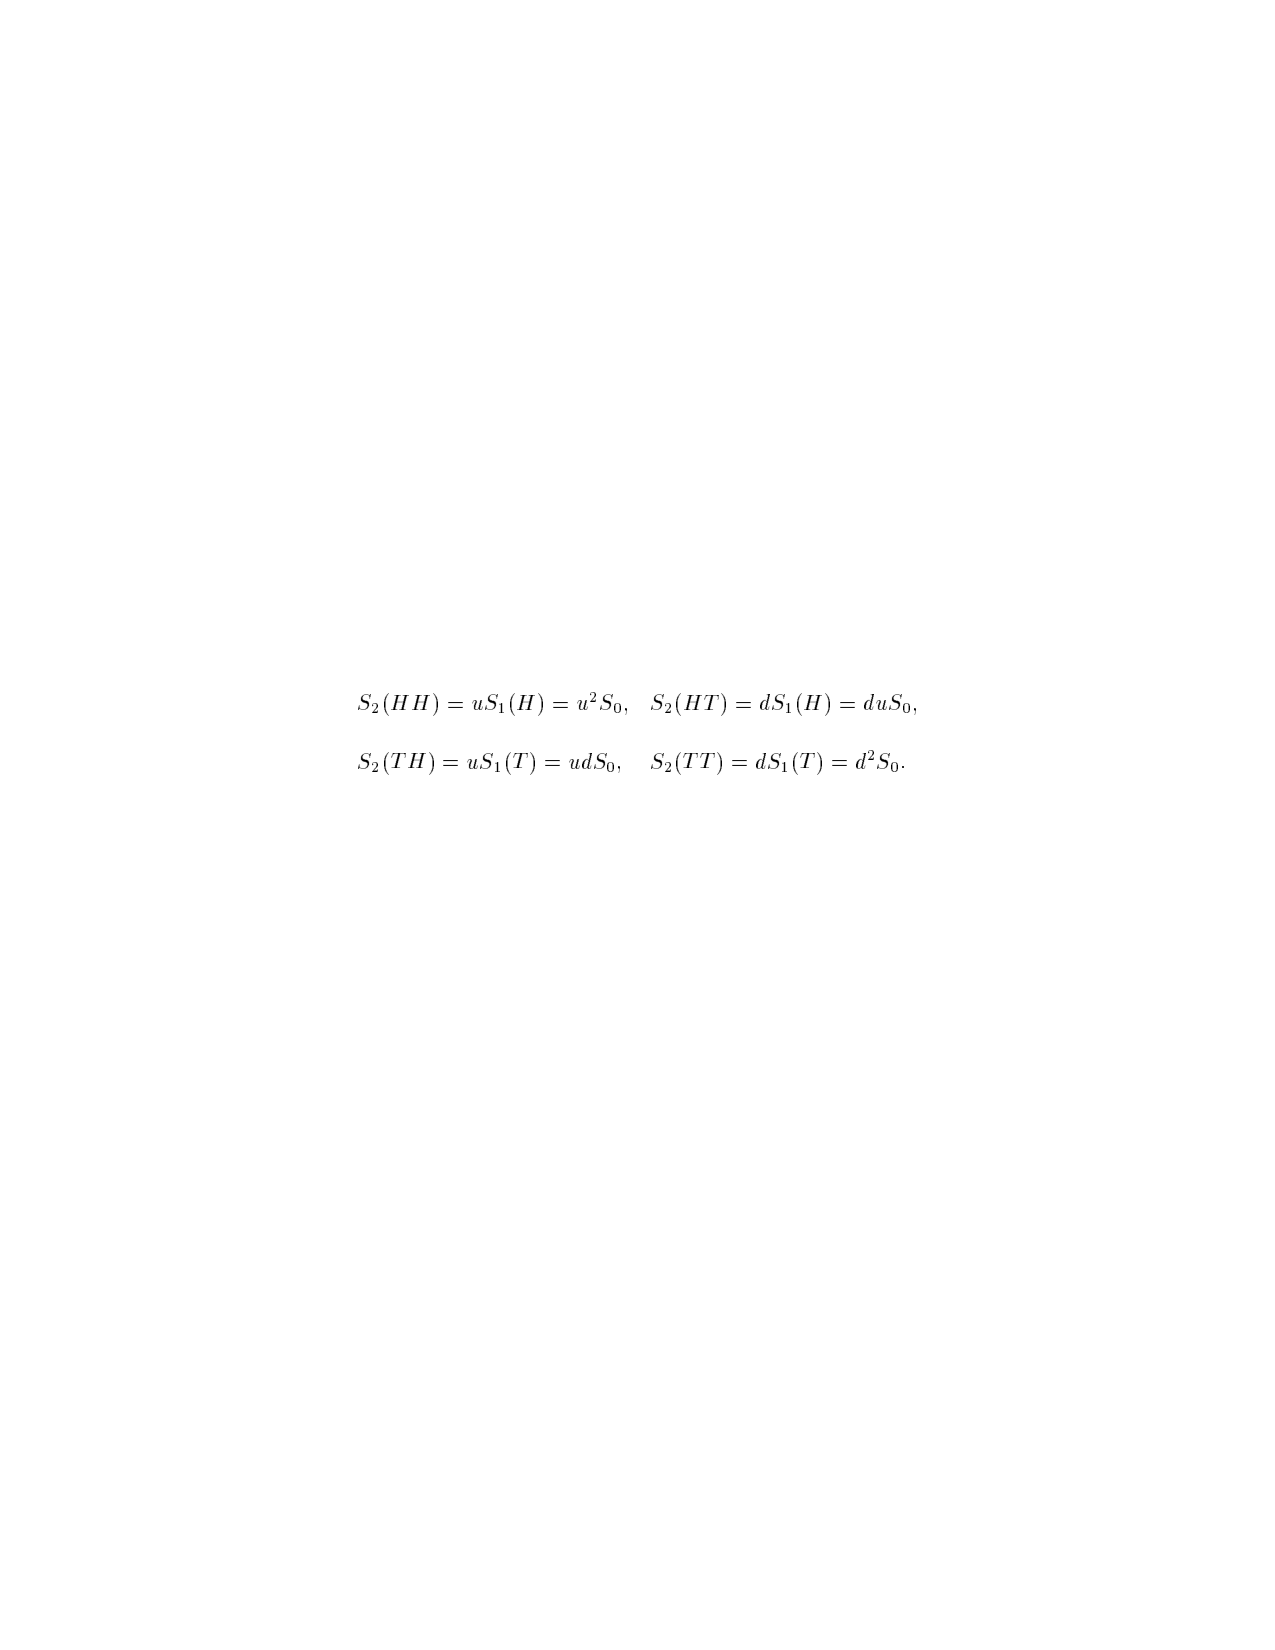
\includegraphics[height=0.75in, width=4in]{Shreve_Bin.pdf}%
\end{figure}%
Indeed, after two tosses, there are four possible coin sequences, 
$$
\{HH,HT,TH,TT\}
$$
although not all of them result in different stock prices at time  $t_2$.
%
%% Define styles for bags and leafs
%\tikzstyle{bag} = [text width=2em, text centered]
%\tikzstyle{end} = []
%\begin{tikzpicture}[sloped]
%   \node (a) at ( 0,0) [bag] {$\$ A$};
%   \node (b) at ( 4,-1.5) [bag] {B};
%   \node (c) at ( 4,1.5) [bag] {C};
%   \node (d) at ( 8,-3) [bag] {D};
%   \node (e) at ( 8,0) [bag] {E};
%   \node (f) at ( 8,3) [bag] {F};
%   \draw [->] (a) to node [below] {$(1-p)$} (b);
%   \draw [->] (a) to node [above] {$P$} (c);
%   \draw [->] (c) to node [below] {$P^2$} (f);
%   \draw [->] (c) to node [above] {$(1-p)p$} (e);
%   \draw [->] (b) to node [below] {$(1-p)p$} (e);
%   \draw [->] (b) to node [above] {$(1-p)^2$} (d);
%\end{tikzpicture}
\end{example}
\end{frame}%





\begin{frame}%
\frametitle{Transformation of discrete random variables}
\begin{example}[cont'd]
Let us set $S_0=1$, $u=2$ and $d=1/2$: we represent the price evolution by a tree:


%
%% Define styles for bags and leafs
\tikzstyle{bag} = [text width=8em, text centered]
\tikzstyle{end} = []
\begin{tikzpicture}[sloped]
   \node (a) at ( 0,0) [bag] {$\$ 1$};
   \node (b) at ( 4,-1.5) [bag] {$\$ d =\$ 0.5$};
   \node (c) at ( 4,1.5) [bag] {$\$ u= \$ 2$};
   \node (d) at ( 8,-3) [bag] {$\$ d^2= \$ 0.25$};
   \node (e) at ( 8,0) [bag] {$\$ ud= \$ du = \$ 1$};
   \node (f) at ( 8,3) [bag] {$\$ u^2=\$ 4$};
   \draw [->] (a) to node [below] {$(1-p)$} (b);
   \draw [->] (a) to node [above] {$p$} (c);
   \draw [->] (c) to node [below] {$p^2$} (f);
   \draw [->] (c) to node [above] {$(1-p)p$} (e);
   \draw [->] (b) to node [below] {$(1-p)p$} (e);
   \draw [->] (b) to node [above] {$(1-p)^2$} (d);
\end{tikzpicture}
\end{example}
\end{frame}%



\begin{frame}%
\frametitle{Transformation of discrete random variables}
\begin{example}[cont'd]
Now consider an European option call with maturity $t_2$ and strike price $K=0.5$, whose random pay-off at $t_2$ is $C=\max(0;S_2-0.5)$. Thus, 
\begin{eqnarray*}
C(HH)=\max(0;4-0.5)=\$ 3.5 & C(HT)=\max(0;1-0.5)=\$ 0.5 \\
C(TH)=\max(0;1-0.5)=\$ 0.5 & C(TT)=\max(0;0.25-0.5)=\$ 0.
\end{eqnarray*}
Thus at maturity $t_2$ we have
\begin{equation*}
\begin{tabular}{l|cll|c}
\multicolumn{2}{l}{\emph{Probability function for }$S_2$} &  & 
\multicolumn{2}{l}{\emph{Probability function for }$C$} \\ 
&  &  &  &  \\ 
$S_2$ & $\Pr \left(\{ X=x_{i} \}\right) =p_{i}$ &  & $C$ & $\Pr \left(\{
C=c_{i}  \}\right) =p_{i}$ \\ \cline{1-2}\cline{4-5}
$\$ u^2$ & $p^2$ & $\qquad \Rightarrow \qquad $ & $\$ 3.5$ & $p^2$
\\ 
$\$ ud$ & $2p(1-p)$ &  & $\$ 0.5$ & $2p(1-p)$ \\ 
%$\$ du$ & $(1-p)p$ &  & $\$ 0.5$ & $(1-p)p$ \\ 
$\$ d^2$ & $(1-p)^2$  &  & $\$ 0$ & $(1-p)^2$%
\end{tabular}%
\end{equation*}
\tiny{Since $ud=du$ the corresponding values of $S_2$ and $C$ can be aggregated, without loss of info.}



\end{example}
\end{frame}%


\begin{frame}%

\frametitle{Transformation of variables using the CDF}

\begin{stepitemize}
\item We can use the same logic for CDF probabilities, whether the random
variables are\textbf{\ discrete or continuous}

\item Let $Y=\psi \left( X\right) $ with $\psi \left( x\right) $ 1-to-1 and
monotone increasing. Then 
\begin{eqnarray*}
F_{Y}\left( y\right) &=&\Pr \left( \{ Y\leq y \}\right) \\
&=&\Pr \left( \{ \psi \left( X\right) \leq y \} \right) =\Pr \left( \{ X\leq \psi
^{-1}\left( y\right) \} \right) \\
&=&F_{X}\left( \psi ^{-1}\left( y\right) \right)
\end{eqnarray*}

\begin{example}
Let $Y=\psi \left( X\right) =\exp^{ X} $ where $%
X\sim F_X$ on all values $x\in 
%TCIMACRO{\U{211d} }%
%BeginExpansion
\mathbb{R}
%EndExpansion
$%
\begin{eqnarray*}
F_{Y}\left( y\right) &=&\Pr \left( \{ Y\leq y \} \right) \\
&=&\Pr \left( \{ \exp^{  X} \leq y \} \right) =\Pr \left( \{ X\leq \ln
\left( y\right) \} \right) \\
&=&F_{X}\left( \ln \left( y\right) \right) \text{ only for }y>0\text{.}
\end{eqnarray*}
\end{example}

%\item True whether $X$ (and hence $Y$) are continuous or discrete random
%variables.
\end{stepitemize}

%TCIMACRO{\TeXButton{EndFrame}{\end{frame}}}%
%BeginExpansion
\end{frame}%
%EndExpansion

%TCIMACRO{\TeXButton{BeginFrame}{\begin{frame}}}%
%BeginExpansion
\begin{frame}%
%EndExpansion

\frametitle{Function 1-to-1 and monotone decreasing}

\begin{stepitemize}
\item Monotone decreasing functions work in a similar way, but require
changing of the inequality sign

\item Let $Y=\psi \left( X\right) $ with $\psi \left( x\right) $ 1-to-1 and 
\textbf{monotone decreasing}. Then 
\begin{eqnarray*}
F_{Y}\left( y\right) &=&\Pr \left( \{ Y\leq y \} \right) \\
&=&\Pr \left( \{ \psi \left( X\right) \leq y \} \right) =\Pr \left( \{ X\geq \psi
^{-1}\left( y\right) \} \right) \\
&=&1-F_{X}\left( \psi ^{-1}\left( y\right) \right)
\end{eqnarray*}

\end{stepitemize}
\begin{example}
Example: let $Y=\psi \left( X\right) =-\exp^ X $ where $%
X\sim F_X$ on all values $x\in 
%TCIMACRO{\U{211d} }%
%BeginExpansion
\mathbb{R}
%EndExpansion
$%
\begin{eqnarray*}
F_{Y}\left( y\right) &=&\Pr \left( \{ Y\leq y \}\right) =\Pr \left( \{ -\exp ^
X \leq y \} \right) \\
&=&\Pr \left( \{ \exp^ X \geq -y \} \right) =\Pr \left( \{ X\geq \ln
\left( -y\right) \} \right) \\
&=&1-F_{X}\left( \ln \left( -y\right) \right) \text{ only for }y<0\text{.}
\end{eqnarray*}
\end{example}


%TCIMACRO{\TeXButton{EndFrame}{\end{frame}}}%
%BeginExpansion
\end{frame}%
%EndExpansion

%TCIMACRO{\TeXButton{BeginFrame}{\begin{frame}}}%
%BeginExpansion
\begin{frame}%
%EndExpansion

\frametitle{Transformation of continuous RV through pdf }

\begin{stepitemize}
\item For continuous random variables, if $\psi \left( x\right) $ 1-to-1 and
monotone \textbf{increasing}, we have%
\begin{equation*}
F_{Y}\left( y\right) =F_{X}\left( \psi ^{-1}\left( y\right) \right)
\end{equation*}

\item Notice this implies that the pdf of $Y=\psi \left( X\right) $ must
satisfy%
\begin{eqnarray*}
f_{Y}\left( y\right) &=&\frac{dF_{Y}\left( y\right) }{dy}=\frac{dF_{X}\left(
\psi ^{-1}\left( y\right) \right) }{dy} \\
&=&\frac{dF_{X}\left( x\right) }{dx}\times \frac{d\psi ^{-1}\left( y\right) 
}{dy}\qquad \text{{\small (chain rule)}} \\
&=&f_{X}\left( x\right) \times \frac{d\psi ^{-1}\left( y\right) }{dy}\qquad 
\text{{\small (derivative of CDF (of }}X\text{){\small \ is pdf)}} \\
&=&f_{X}\left( \psi ^{-1}\left( y\right) \right) \times \frac{d\psi
^{-1}\left( y\right) }{dy}\qquad \text{{\small (substitute }}x=\psi
^{-1}\left( y\right) \text{{\small )}}
\end{eqnarray*}
\end{stepitemize}

%TCIMACRO{\TeXButton{EndFrame}{\end{frame}}}%
%BeginExpansion
\end{frame}%
%EndExpansion

%TCIMACRO{\TeXButton{BeginFrame}{\begin{frame}}}%
%BeginExpansion
\begin{frame}%
%EndExpansion

\frametitle{Transformation of continuous RV through pdf }

\begin{stepitemize}
\item What happens when $\psi \left( x\right) $ 1-to-1 and monotone \textbf{%
decreasing}? We have%
\begin{equation*}
F_{Y}\left( y\right) =1-F_{X}\left( \psi ^{-1}\left( y\right) \right)
\end{equation*}

\item So now the pdf of $Y=\phi \left( X\right) $ must satisfy 
\begin{eqnarray*}
f_{Y}\left( y\right) &=&\frac{dF_{Y}\left( y\right) }{dy}=-\frac{%
dF_{X}\left( \psi ^{-1}\left( y\right) \right) }{dy} \\
&=&-f_{X}\left( \psi ^{-1}\left( y\right) \right) \times \frac{d\psi
^{-1}\left( y\right) }{dy}\qquad \text{{\small (same reasons as before)}}
\end{eqnarray*}

\item but $\frac{d\psi ^{-1}\left( y\right) }{dy}<0$ since here $\psi \left(
\cdot \right) $ is monotone decreasing, hence we can write%
\begin{equation*}
f_{Y}\left( y\right) =f_{X}\left( \psi ^{-1}\left( y\right) \right) \times
\left\vert \frac{d\psi ^{-1}\left( y\right) }{dy}\right\vert
\end{equation*}

\item This expression (called Jacobian-formula) is valid for $\psi \left( x\right) $ 1-to-1 and
monotone (whether increasing or decreasing)
\end{stepitemize}

%TCIMACRO{\TeXButton{EndFrame}{\end{frame}}}%
%BeginExpansion
\end{frame}%
%EndExpansion

%TCIMACRO{\TeXButton{BeginFrame}{\begin{frame}}}%
%BeginExpansion
\begin{frame}%
%EndExpansion

\frametitle{Example of transformation using pdf}

\begin{example}
\begin{stepitemize}
\item So what is the pdf for the lognormal distribution?

\item Recall that $Y$ has a \textbf{lognormal distribution} when $\ln \left(
Y\right) =X$ has a Normal distribution

\item $\Rightarrow $ if $X\sim \N\left( \mu ,\sigma ^{2}\right) ,$ then $%
Y=\exp^X\sim $ \emph{lognormal}$\left( \mu ,\sigma ^{2}\right) $

\begin{stepitemize}
\item Corresponding to $\psi \left( x\right) =\exp^x$ and $\psi
^{-1}\left( y\right) =\ln (y)$
\end{stepitemize}

\item The \emph{pdf} of $X$ is 
\begin{equation*}
f_{X}\left( x\right) =\frac{1}{\sqrt{2\pi \sigma ^{2}}}\exp^{ \left\{ -\frac{1%
}{2\sigma ^{2}}\left( x-\mu \right) ^{2}\right\}}
\end{equation*}%
for any $-\infty <x<\infty $

\item Using $\psi \left( x\right) =\exp^x$ we know we'll have possible
values for $Y$ only on $0<y<\infty $
\end{stepitemize}
\end{example}
%TCIMACRO{\TeXButton{EndFrame}{\end{frame}}}%
%BeginExpansion
\end{frame}%
%EndExpansion

%TCIMACRO{\TeXButton{BeginFrame}{\begin{frame}}}%
%BeginExpansion
\begin{frame}%
%EndExpansion

\frametitle{Example of transformation using pdf}
\begin{example}[cont'd]
\begin{stepitemize}
\item We know that 
\begin{equation*}
f_{Y}\left( y\right) =f_{X}\left( \psi ^{-1}\left( y\right) \right) \times
\left\vert \frac{d\psi ^{-1}\left( y\right) }{dy}\right\vert
\end{equation*}

\item And since $\psi ^{-1}\left( y\right) =\ln (y)$ then 
\begin{equation*}
\left\vert \frac{d\psi ^{-1}\left( y\right) }{dy}\right\vert =\left\vert 
\frac{1}{y}\right\vert
\end{equation*}

\item $\Rightarrow $ the \emph{pdf} of $Y$ is 
\begin{equation*}
f_{Y}\left( y\right) =\frac{1}{y\sqrt{2\pi \sigma ^{2}}}\exp^{ \left\{ -\frac{1%
}{2\sigma ^{2}}\left( \ln (y)-\mu \right) ^{2}\right\}}
\end{equation*}%
for any $0<y<\infty $
\end{stepitemize}
\end{example}
%TCIMACRO{\TeXButton{EndFrame}{\end{frame}}}%
%BeginExpansion
\end{frame}

\begin{frame}

\frametitle{Example of transformation using pdf}
\begin{example}[cont'd]
\begin{stepitemize}
\item Both the Normal and the lognormal are characterized by
only two parameters ($\mu$ and $\sigma$). The \emph{median} of the lognormal distribution is $\exp^{
\mu } $, since $$
\Pr \left( \{ X\leq \mu \} \right) = 0.5, 
$$
and hence%
\begin{eqnarray*}
0.5 &=&\Pr \left(\{ X\leq \mu \}\right) \\
&=&\Pr \left( \{\exp^{X} \leq \exp^{ \mu }\} \right) \\
&=&\Pr \left( \{Y\leq \exp^{ \mu }\} \right).
\end{eqnarray*}
\end{stepitemize}
\end{example}
More generally, for $\alpha\in[0,1]$, the $\alpha$-th quantile of a r.v. $X$ is the value $x_\alpha$ such that $P(\{X \leq x_\alpha\})\geq\alpha$. If $X$ si a continuous r.v.  we can set $P(\{X \leq x_\alpha\})=\alpha$ (as we did, e.g., for the lognormal).
\end{frame}

\begin{frame}
\frametitle{A caveat }

When $X$ and $Y$ are two random variables, we should pay attention to their transformations. For instance, let us consider
$$
X\sim \mathcal{N}(\mu,\sigma^2) \quad \text{and}  \quad Y\sim Exp(\lambda).
$$ 
Then, let's transform $X$ and $Y$

\begin{itemize}
\item  in a linear way: $Z=X+Y$. We know that 
$$
E[Z] = E[X+Y] = E[X] + E[Y] 
$$
%so we can rely on the linearity of the expected value.
\item in a nonlinear way $W = X/Y$. One can show that
$$\color{red}
E[W] = E\left[\frac{X}{Y}\right] \neq \frac{E[X]}{E[Y]}. \color{black}
$$
%so, we cannot rely on the linearity of the expected value.
 \end{itemize}
\end{frame}

\begin{frame}
\frametitle{The big picture}

Despite exotic names, the common distributions relate to each other in intuitive and interesting ways. Several follow naturally from the Bernoulli distribution, for example. 

\begin{figure}[ptb]\centering
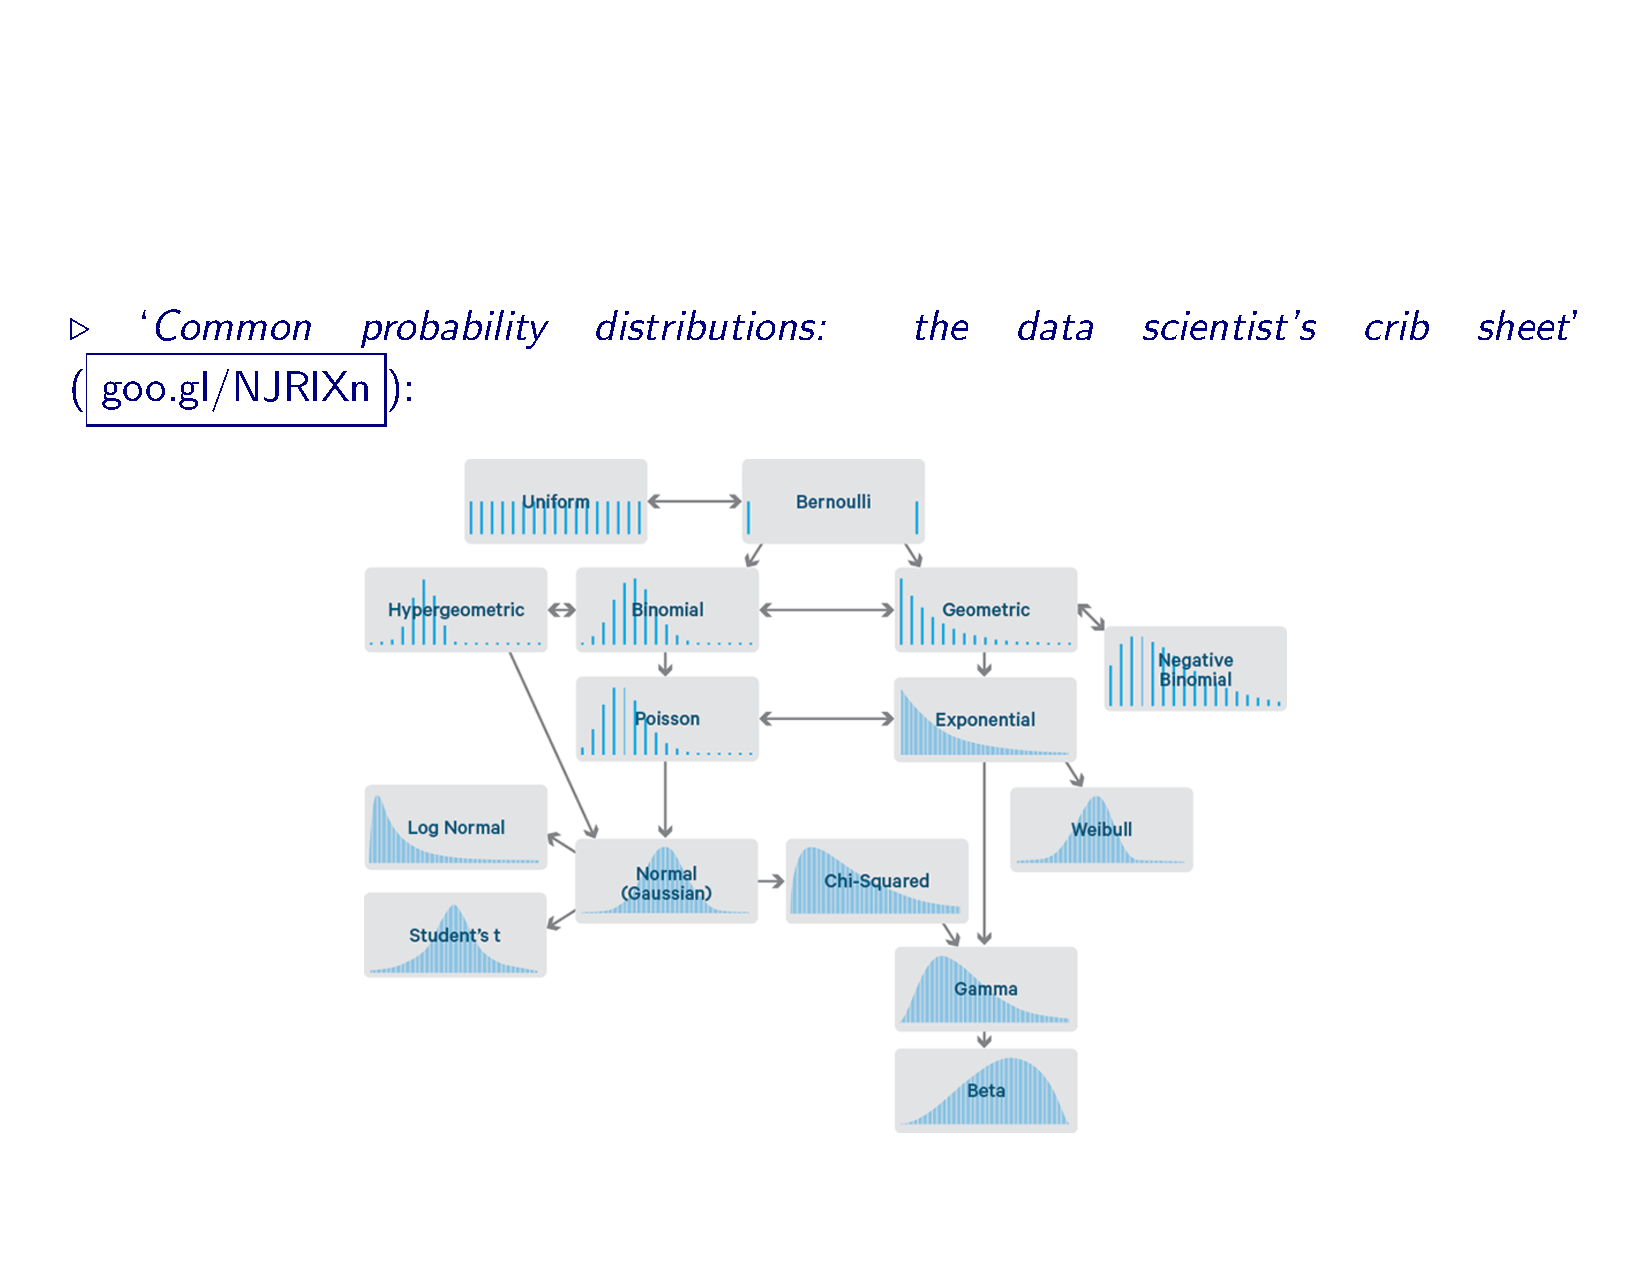
\includegraphics[height=2.3in, width=4.5in]{RelRVs_Diego.pdf}%
\end{figure}%

\end{frame}




\end{document}





%
%
%To calculate $Pr(X\leq x)$ we also use the standard normal density
%function (Integration by substitution once again):
%\begin{eqnarray*}
%Pr(X\leq
%x)&=&\int_{-\infty}^x\frac{1}{\sqrt{2\pi\sigma^2}}\exp\{-\frac{(t-\mu)^2}{2\sigma^2}\}dt\\
% &=&\int_{-\infty}^z\phi(s)ds
%\end{eqnarray*}
%where $z=(x-\mu)/\sigma$, $s=(t-\mu)/\sigma$ and $ds=dt/\sigma$.
%We can then evaluate the probabilities
%$$
%Pr(Z\leq z)=\int_{-\infty}^z\phi(s)ds
%$$
%either directly using a computer or indirectly via Standard Normal
%Tables.  Standard Normal Tables give values of
%$$
%\Phi(z)=\int_{-\infty}^z\phi(s)ds
%$$
%for various values of $z\geq 0$. (The tables are themselves
%calculated using a computer, of course.) For negative values of
%$z$ the symmetry property of $\phi(z)$ (\textit{i.e.}
%$\phi(z)=\phi(-z)$) tells us that
%$$
%\Phi(-z)=1-\Phi(z)~.
%$$
%Hence we can evaluate $Pr(X\leq x)$ for all values of $x$.
%Similarly,
%\begin{eqnarray*}
%Pr(x_1<X\leq x_2)&=&Pr(z_1<Z\leq z_2)\\
% &=&\Phi(z_2)-\Phi(z_1)
% \end{eqnarray*}
%where $z_1=(x_1-\mu)/\sigma$ and $z_2=(x_2-\mu)/\sigma$.
